\documentclass[sn-mathphys,Numbered]{sn-jnl}
\usepackage{graphicx}
\usepackage{multirow}
\usepackage{amsmath,amssymb,amsfonts}
\usepackage{amsthm}
\usepackage{subcaption}
\usepackage{mathrsfs}
\usepackage[title]{appendix}
\usepackage{xcolor}
\usepackage{textcomp}
\usepackage{manyfoot}
%\usepackage{subfig}
\usepackage{booktabs}
\usepackage{algorithm}
\usepackage{algorithmicx}
\usepackage{algpseudocode}
\usepackage{listings}
\theoremstyle{thmstyleone}
\newtheorem{theorem}{Theorem}
\newtheorem{proposition}[theorem]{Proposition}
\theoremstyle{thmstyletwo}
\newtheorem{example}{Example}
\newtheorem{remark}{Remark}
\theoremstyle{thmstylethree}
\newtheorem{definition}{Definition}
\raggedbottom

\begin{document}
\title[Article Title]{Temperature Prediction using Deep Learning Models: A Paradigm Shift}
\author*[1,2]{\fnm{Rana} \sur{Kumar}}\email{singhranakumar22@gmail.com}
\author[1,2]{\fnm{Vipin} \sur{Kumar}}\email{rt.vipink@gmail.com}
%\equalcont{These authors contributed equally to this work.}

%\author[1,2]{\fnm{Third} \sur{Author}}\email{iiiauthor@gmail.com}
%\equalcont{These authors contributed equally to this work.}

\affil*[1]{\orgdiv{Computer Science \& Information Technology}, \orgname{Mahatma Gandhi Central University}, \orgaddress{\state{Bihar}, \country{India}}}

%\affil[2]{\orgdiv{Computer Science \& Information Technology}, \orgname{Mahatma Gandhi Central University}, \orgaddress{\state{Bihar}, \country{India}}}

%\affil[3]{\orgdiv{Department}, \orgname{Organization}, \orgaddress{\street{Street}, \city{City}, \postcode{610101}, \state{State}, \country{Country}}}

%%==================================%%
%% sample for unstructured abstract %%
%%==================================%%

\abstract{Accurate temperature prediction holds key significance in distinct sectors such as power requirement in city and industry, with deep implications for global climate understanding. This paper presents an innovative approach to enhance the temperature prediction through the vareious deep learning techniques: Long Short-Term Memory (LSTM), Recurrent Neural Networks (RNN), Gated Recurrent Unit (GRU) and Bidirectional Long Short-Term Memory (BiLSTM). These deep learning techniques have capability in capturing complex temporal dependencies complements \cite{xu2019improving} , modifying overfitting concerns. The proposed Paradigm Shift hybrid models capitalizes on the strengths of traditional deep learning methods, seeking to boost their predictive capability and reduce variance-related errors.

Our study dig in into the complex stuff of time-series satellite data, particularly focusing on Delhi city temperature deviation. Informed by the relatively indefinite variation of City Temperature, we influence Paradigm Shift to get new shifted dataset. Traditional BI LSTM (BI-LSTM) is introduced, enhancing the predictive power by placing emphasis on local data interactions \cite{tabrizi2021hourly}. The BI-LSTM methodology performs the best because it adopts a quadratic cost function and strategically weighting training sample data proximate to test different point.}



\keywords{Time-Series, Deep Learning, LSTM, BI-LSTM, GRU, RNN}

%%\pacs[JEL Classification]{D8, H51}

%%\pacs[MSC Classification]{35A01, 65L10, 65L12, 65L20, 65L70}

\maketitle

\section{Introduction}\label{sec1}

Temperature prediction is a fundamental aspect of weather forecasting and climate research, essential for various applications across diverse domains, ranging from agriculture and energy management to public health planning and urban infrastructure development. Accurate temperature forecasts enable us to make informed decisions, proactively respond to extreme weather events, and adapt to changing climate patterns. While traditional statistical methods have been the cornerstone of weather prediction, recent advancements in deep learning have opened up new avenues for enhancing the accuracy and reliability of temperature forecasting. Likewise, impacts on the food security, human health, economy, and energy consumption are anticipated \cite{cifuentes2020air}.

In this paper, we delve into the application of deep learning techniques for temperature prediction using time series data from the bustling metropolis of Delhi, India. Delhi, being the capital city and one of the most populous urban centers in India, experiences diverse weather patterns influenced by both natural climate variability and anthropogenic activities. Understanding and predicting temperature trends in this region is crucial for effective urban planning, resource management, and mitigating the impacts of heatwaves and cold spells on public health and infrastructure. air temperature prediction is a main climatic factor needed for many different applications in multiple area such as tourism, agriculture,  industry,  environment,  energy etc \cite{abdel2004hourly}. 
Through this paper, we aim to investigate the effectiveness of employing deep learning models in predicting temperature patterns in Delhi. By utilizing historical temperature data collected from various meteorological stations, we seek to train and evaluate the performance of deep learning models and compare their results with traditional forecasting methods. The insights gained from this study will shed light on the strengths and limitations of deep learning-based temperature predictions and provide valuable guidance for future research and practical implementations.
\subsection{The novelty of proposed research work:}

\begin{itemize}
\item A comprehensive performance study of different measures of the Deep Learning Models has been done where the better performer has been identified successfully based on RMSE,MAE. Now our goal is to develop a hybrid model which have better value of RMSE,MAE to predict better result.
\end{itemize}
The remainder of this paper is organised as follows: Section 2 provides a review of the literature, as well as a list of recent works. Section 3 gives the problem description and research goals. Section 4 includes an example of the data collection as well as the experimental design as an experiment. Section 5 presents the experimental results and their thorough analysis. The sixth section concluded with a review of existing and future research endeavours.

\section{Previous Work}
Many research has been undertaken to predict temperature using past data as a critical temperature attribute. Researchers require effective study and data to procced their investigation on a dataset of temperature of city \cite{cifuentes2020air}. The temperature is used as a parameter to identify the climate change,  green house effect, crop yield etc.
\cite{2019AGUFMGC33A..05P}This study explored the application of deep learning models for extreme weather prediction, including temperature extremes. Extreme weather events, such as heatwaves and cold spells, have significant impacts on society and require accurate forecasting for effective preparation and response. The authors experimented with LSTM networks and Convolutional Neural Networks (CNNs) to predict extreme weather events. LSTMs were employed to capture temporal dependencies, while CNNs were used to extract spatial patterns from meteorological data. The research demonstrated that deep learning models outperformed traditional methods in predicting temperature extremes, showcasing the potential of these models in enhancing weather forecasting systems to address severe weather events.

This work introduced DeepAR, a probabilistic forecasting model based on autoregressive recurrent networks. The model is capable of providing not only point predictions but also probability distributions for uncertainty estimation. For temperature prediction, uncertainty estimation is crucial, as it provides valuable information for decision-making in weather-sensitive applications. DeepAR offers a principled approach for capturing the uncertainty in predictions, making it suitable for applications where risk assessment is important \cite{salinas2020deepar}.

This paper addresses the temporal and time-series nature of temperature prediction and its critical role in today's agricultural and industrial sectors. Leveraging neural networks due to the non-linearities in climatic physics, the paper introduces a significant approach: the integration of backpropagation with genetic algorithms for training these networks. The central contribution is a time series-based temperature prediction model employing this integrated technique.The paper's focus includes demonstrating the interdependence of temperature and specific data sequences, emphasizing the implications of accurate forecasting for key sectors. It further explores the suitability of neural networks in capturing intricate meteorological processes. The proposed technique sheds light on the effects of undertraining and overtraining, highlighting the model's sensitivity to proper training \cite{singh2011time}.

 This paper proposes a novel approach for predicting short and mid-term daily sea surface temperature anomalies (SSTA) using a combination of the LSTM deep recurrent neural network model and the AdaBoost ensemble learning model (LSTM-AdaBoost). The goal is to improve predictive accuracy by leveraging LSTM's ability to capture long-term dependencies and AdaBoost's robust prediction capability, while mitigating overfitting. The method involves modeling SSTA seasonality, training LSTM and AdaBoost independently, and combining their predictions using an averaging strategy. The study demonstrates the effectiveness of the LSTM-AdaBoost model in outperforming individual LSTM, AdaBoost, and other optimized models, offering promising potential for enhancing short and mid-term daily SST predictions in scenarios like extreme weather events \cite{XIAO2019111358}.

 The paper highlights the effectiveness of Long Short-Term Memory (LSTM) in capturing long-term dependencies, particularly in weather forecasting applications. Additionally, the study introduces Transductive LSTM (T-LSTM) as a novel approach that leverages local information in time-series prediction. T-LSTM operates in a transductive learning framework, attributing higher influence to nearby samples during model fitting. A quadratic cost function is used for regression, with the objective function localized by assigning larger weights to training samples near the test point. Two weighting schemes, based on cosine similarity, are explored \cite{XIAO2019111358}.
The research evaluates the proposed method's performance across varying weather conditions, conducting experiments over two different time periods within a year. The findings demonstrate that T-LSTM exhibits superior predictive performance compared to traditional LSTM, establishing its effectiveness in enhancing prediction accuracy for weather forecasting tasks.

\begin{table}[h]
\caption{Literature Review Of Other Papers}\label{tab1}%
\begin{tabular}{@{}lllll@{}}
\toprule
Paper & MODELS  & Data Set Used & RMSE(°C) & MSE(°C) \\
\midrule
\cite{li2019deep}    & LSTM   & china international airport temperature data from 2009-2018  &1.2369 &1.5365    \\
\cite{li2019deep}   & Random Forest   & china international airport temperature data from 2009-2018  &1.3612 &1.8645     \\
\cite{xiao2019spatiotemporal}    & LSTM   & East China Sea surface temperature data from 1982-2018   & 0.850 & -  \\
\cite{thi2020deep}  & RNN       & Winter data of south korea from 1976-2015.     & 2.985      & 2.5777    \\
\cite{thi2020deep}  & LSTM    & Winter data of south korea from 1976-2015.      & 2.991       & 2.5525 \\
\botrule
\end{tabular}
%\footnotetext{Source: This is an example of table footnote. This is an example of table footnote.}
%\footnotetext[1]{Example for a first table footnote. This is an example of table footnote.}
%\footnotetext[2]{Example for a second table footnote. This is an example of table footnote.}
\end{table}
\section{Deep Learning Models And Performance Measures:}

\subsection {Recurrent neural networks (RNN):}
Recurrent neural networks (RNN) are a ANN, where the outputs of past steps are fed as inputs to the current phase. The unique feature of RNN is the feedback connection that transmits information about the previous input, which is adapted to the next input. RNN also have a hidden state vector or memory that retrieves some sequence data and computes new states by recursively applying its activation functions to previous states and new inputs (see Figure 1b). In this way, the RNN can process information sequentially and represent a temporal behavior for a time series, preserving information from previous data \cite{thi2020deep}.
The equation for a simple Recurrent Neural Network (RNN) is as follows:
\begin{equation}
h_t=\sigma(W_{hh} \cdot h_{t-1} + W_{hx} \cdot x_t + b_h)
\end{equation}

Where:
\begin{itemize}
\item \(x_t\) represents the input at time step \(t\).
\item \(h_t\) is the hidden state at time step \(t\).
\item \(W_{hh}\) is the weight matrix for the recurrent connection.
\item \(W_{hx}\) is the weight matrix for the input connection.
\item \(b_h\) is the bias vector.
\item \(\sigma\) is the activation function, commonly the sigmoid function.
\end{itemize}
\subsection{GRU}

The Gated Recurrent Unit (GRU) is a neural network design addressing vanishing gradient challenges in sequence data modeling. It employs update and reset gates to control information flow within the network. The update gate balances new input against the previous state, while the reset gate decides what past information to ignore. The model's computations involve gate calculations, generating a candidate hidden state, and merging it with the previous state using the update gate. This architecture efficiently captures temporal patterns and long-range dependencies, making it popular for tasks involving sequential data like natural language processing and time series analysis. Its simplified structure and effectiveness offer an alternative to more complex architectures like LSTM. Equations of GRU are as follows:
\begin{equation}
z_t = \sigma(W_z \cdot [h_{t-1}, x_t] + b_z) 
\end{equation}
\begin{equation}
r_t = \sigma(W_r \cdot [h_{t-1}, x_t] + b_r) 
\end{equation}
\begin{equation}
\tilde{h}_t = \tanh(W_h \cdot [r_t \odot h_{t-1}, x_t] + b_h) \\
\end{equation}
\begin{equation}
h_t = (1 - z_t) \odot h_{t-1} + z_t \odot \tilde{h}_t
\end{equation}



Where:
\begin{itemize}
\item \(x_t\) represents the input at time step \(t\).
\item \(h_t\) is the hidden state at time step \(t\).
\item \(z_t\) is the update gate's output at time step \(t\).
\item \(r_t\) is the reset gate's output at time step \(t\).
\item \(\tilde{h}_t\) is the candidate hidden state at time step \(t\).
\item \(W_z\), \(W_r\), and \(W_h\) are weight matrices for the update gate, reset gate, and candidate hidden state calculations, respectively.
\item \(b_z\), \(b_r\), and \(b_h\) are bias vectors for the corresponding gates and candidate hidden state.
\item \(\sigma\) is the sigmoid activation function.
\item \(\odot\) represents element-wise multiplication.
\end{itemize}

\subsection{Long Short Term Memory}
Long Short-Term Memory (LSTM) is a specialized recurrent neural network architecture addressing vanishing gradient problems. It introduces memory cells and three gates: input, output, and forget. The input gate regulates new information intake, the output gate controls the information output, and the forget gate manages the memory's relevance. The cell state maintains long-term dependencies, enhancing the model's ability to capture sequences \cite{guillen2020deep}. LSTMs address challenges faced by traditional RNNs by allowing selective information update through gates and consistent gradient flow. This architecture is widely used for sequential data tasks, like language translation and speech recognition, due to its capacity for modeling context and handling extended sequences effectively \cite{qiu2021river}. The equations of LSTM are as follows:
\begin{equation}
f_t = \sigma(W_f \cdot [h_{t-1}, x_t] + b_f)
\end{equation}
\begin{equation}
i_t = \sigma(W_i \cdot [h_{t-1}, x_t] + b_i)
\end{equation}
\begin{equation}
\tilde{C}_t = \tanh(W_C \cdot [h_{t-1}, x_t] + b_C)
\end{equation}
\begin{equation}
C_t = f_t \odot C_{t-1} + i_t \odot \tilde{C}_t
\end{equation}
\begin{equation}
o_t = \sigma(W_o \cdot [h_{t-1}, x_t] + b_o)
\end{equation}
\begin{equation}
h_t = o_t \odot \tanh(C_t)
\end{equation}


Where:
\begin{itemize}
\item \(x_t\) represents the input at time step \(t\).
\item \(h_t\) is the hidden state at time step \(t\).
\item \(C_t\) is the cell state at time step \(t\).
\item \(f_t\) is the forget gate's output at time step \(t\).
\item \(i_t\) is the input gate's output at time step \(t\).
\item \(\tilde{C}_t\) is the candidate cell state at time step \(t\).
\item \(o_t\) is the output gate's output at time step \(t\).
\item \(W_f\), \(W_i\), \(W_C\), and \(W_o\) are weight matrices for the gates and candidate cell state calculations.
\item \(b_f\), \(b_i\), \(b_C\), and \(b_o\) are bias vectors for the corresponding gates and candidate cell state.
\item \(\sigma\) is the sigmoid activation function.
\item \(\odot\) represents element-wise multiplication.
\end{itemize}

\subsection{Bidirectional Long Short-Term Memory (BiLSTM)}
Bidirectional Long Short-Term Memory (BiLSTM) is an advanced neural network structure that overcomes vanishing gradient issues by processing data in both forward and backward directions. It consists of two LSTMs: one captures past information, and the other captures future context. Input sequences are processed in parallel, enabling the model to capture comprehensive temporal patterns. BiLSTMs are powerful for tasks demanding context understanding, like named entity recognition and sentiment analysis. They provide a holistic view of input data, enhancing the network's ability to capture dependencies and improving performance in various sequence-related tasks.
The equations for the Bidirectional Long Short-Term Memory (BiLSTM) network are as follows:

\textbf{Forward LSTM:}
\begin{equation}
f_t^{(\text{forward})} = \sigma(W_{f}^{(\text{forward})} \cdot [h_{t-1}^{(\text{forward})}, x_t] + b_{f}^{(\text{forward})})
\end{equation}
\begin{equation}
i_t^{(\text{forward})} = \sigma(W_{i}^{(\text{forward})} \cdot [h_{t-1}^{(\text{forward})}, x_t] + b_{i}^{(\text{forward})})
\end{equation}
\begin{equation}
\tilde{C}_t^{(\text{forward})} = \tanh(W_{C}^{(\text{forward})} \cdot [h_{t-1}^{(\text{forward})}, x_t] + b_{C}^{(\text{forward})})
\end{equation}
\begin{equation}
C_t^{(\text{forward})} = f_t^{(\text{forward})} \odot C_{t-1}^{(\text{forward})} + i_t^{(\text{forward})} \odot \tilde{C}_t^{(\text{forward})}
\end{equation}
\begin{equation}
o_t^{(\text{forward})} = \sigma(W_{o}^{(\text{forward})} \cdot [h_{t-1}^{(\text{forward})}, x_t] + b_{o}^{(\text{forward})})
\end{equation}
\begin{equation}
h_t^{(\text{forward})} = o_t^{(\text{forward})} \odot \tanh(C_t^{(\text{forward})})
\end{equation}

\textbf{Backward LSTM:}
\begin{equation}
f_t^{(\text{backward})} = \sigma(W_{f}^{(\text{backward})} \cdot [h_{t+1}^{(\text{backward})}, x_t] + b_{f}^{(\text{backward})})
\end{equation}
\begin{equation}
i_t^{(\text{backward})} = \sigma(W_{i}^{(\text{backward})} \cdot [h_{t+1}^{(\text{backward})}, x_t] + b_{i}^{(\text{backward})})
\end{equation}
\begin{equation}
\tilde{C}_t^{(\text{backward})} = \tanh(W_{C}^{(\text{backward})} \cdot [h_{t+1}^{(\text{backward})}, x_t] + b_{C}^{(\text{backward})})
\end{equation}
\begin{equation}
C_t^{(\text{backward})} = f_t^{(\text{backward})} \odot C_{t+1}^{(\text{backward})} + i_t^{(\text{backward})} \odot \tilde{C}_t^{(\text{backward})}
\end{equation}
\begin{equation}
o_t^{(\text{backward})} = \sigma(W_{o}^{(\text{backward})} \cdot [h_{t+1}^{(\text{backward})}, x_t] + b_{o}^{(\text{backward})})
\end{equation}
\begin{equation}
h_t^{(\text{backward})} = o_t^{(\text{backward})} \odot \tanh(C_t^{(\text{backward})})
\end{equation}

Where:
\begin{itemize}
\item \(x_t\) represents the input at time step \(t\).
\item \(h_t^{(\text{forward})}\) and \(h_t^{(\text{backward})}\) are the hidden states of the forward and backward LSTMs at time step \(t\), respectively.
\item \(C_t^{(\text{forward})}\) and \(C_t^{(\text{backward})}\) are the cell states of the forward and backward LSTMs at time step \(t\), respectively.
\item \(f_t^{(\text{forward})}\) and \(f_t^{(\text{backward})}\) are the forget gate's outputs of the forward and backward LSTMs at time step \(t\), respectively.
\item \(i_t^{(\text{forward})}\) and \(i_t^{(\text{backward})}\) are the input gate's outputs of the forward and backward LSTMs at time step \(t\), respectively.
\item \(\tilde{C}_t^{(\text{forward})}\) and \(\tilde{C}_t^{(\text{backward})}\) are the candidate cell states of the forward and backward LSTMs at time step \(t\), respectively.
\item \(o_t^{(\text{forward})}\) and \(o_t^{(\text{backward})}\) are the output gate's outputs of the forward and backward LSTMs at time step \(t\), respectively.
\item \(W_{f}^{(\text{forward})}\), \(W_{i}^{(\text{forward})}\), \(W_{C}^{(\text{forward})}\), and \(W_{o}^{(\text{forward})}\) are weight matrices for the gates and candidate cell state calculations of the forward LSTM.
\item \(W_{f}^{(\text{backward})}\), \(W_{i}^{(\text{backward})}\), \(W_{C}^{(\text{backward})}\), and \(W_{o}^{(\text{backward})}\) are weight matrices for the gates and candidate cell state calculations of the backward LSTM.
\item \(b_{f}^{(\text{forward})}\), \(b_{i}^{(\text{forward})}\), \(b_{C}^{(\text{forward})}\), and \(b_{o}^{(\text{forward})}\) are bias vectors for the corresponding gates and candidate cell state of the forward LSTM.
\item \(b_{f}^{(\text{backward})}\), \(b_{i}^{(\text{backward})}\), \(b_{C}^{(\text{backward})}\), and \(b_{o}^{(\text{backward})}\) are bias vectors for the corresponding gates and candidate cell state of the backward LSTM.
\item \(\sigma\) is the sigmoid activation function.
\item \(\odot\) represents element-wise multiplication.
\end{itemize}

\subsection {Performance Measures:}
\subsubsection{Root Mean Squared Error (RMSE)}:
It is a widely used performance metric in regression tasks, including temperature prediction. It measures the average magnitude of the errors between predicted and actual values. RMSE is calculated by taking the square root of the mean of the squared differences between predicted and actual values.

The formula for RMSE is as in equation \ref{eqn:e}:
\begin{equation}
\label{eqn:e}
RMSE = \sqrt {\frac{1}{N} \sum_{i=1}^{N} (\hat{y_{i}} - y_{i})^2}
\end{equation}
Where the variables $\hat{y}_i$ is predicted values of the target variable (e.g., temperature), $y_i$ is the Actual values of the target variable and N is the number of data points in the dataset.
\subsubsection {Mean Squared Error (MSE):}
Mean Squared Error (MSE) is another widely used performance metric in regression tasks, including temperature prediction. It measures the average of the squared differences between predicted and actual values. MSE emphasizes larger errors more than smaller errors due to the squaring of the differences.
The formula for MSE is as depicted in equation \ref{eqn:mse}
\begin{equation}
\label{eqn:mse}
MSE = \frac{1}{N} \sum_{i=1}^{N} (\hat{y_{i}} - y_{i})^2
\end{equation}
Where the variables $\hat{y}_i$ is predicted values of the target variable (e.g., temperature), $y_i$ is the Actual values of the target variable and N is the number of data points in the dataset.

\subsubsection {Mean Absolute Error (MAE):} It is a data dependent performance metric used for evaluation of average of exact error between actual and predicted variables. The formula for MAE is depicted in equation \ref{eqn:mae}
\begin{equation}
\label{eqn:mae}
MAE = \frac{1}{N} \sum_{i=1}^{N} \mid\hat{y_{i}} - y_{i}\mid .
\end{equation}
Where the variables $\hat{y}_i$ is predicted values of the target variable (e.g., temperature), $y_i$ is the Actual values of the target variable and N is the number of data points in the dataset.
\subsubsection {Mean Absolute Percentage Error (MAPE):}
Mean Absolute Percentage Error (MAPE) is a performance metric commonly used in regression tasks, including temperature prediction. It measures the average percentage difference between predicted and actual values, providing a relative measure of the accuracy of the model's predictions.

The formula for MAPE is represented in equation \ref{eqn:mape}
\begin{equation}
\label{eqn:mape}
MAPE = \frac{100}{N} \sum_{i=1}^{N} \mid(\frac{\hat{y_{i}} - y_{i}}{y_i})\mid .
\end{equation}

%MAPE = (1/n) * Σ(|(y_actual - y_pred) / y_actual|) * 100

Where the variables $\hat{y}_i$ is predicted values of the target variable (e.g., temperature), $y_i$ is the Actual values of the target variable and N is the number of data points in the dataset.

\begin{figure}[ht!]
    \centering
    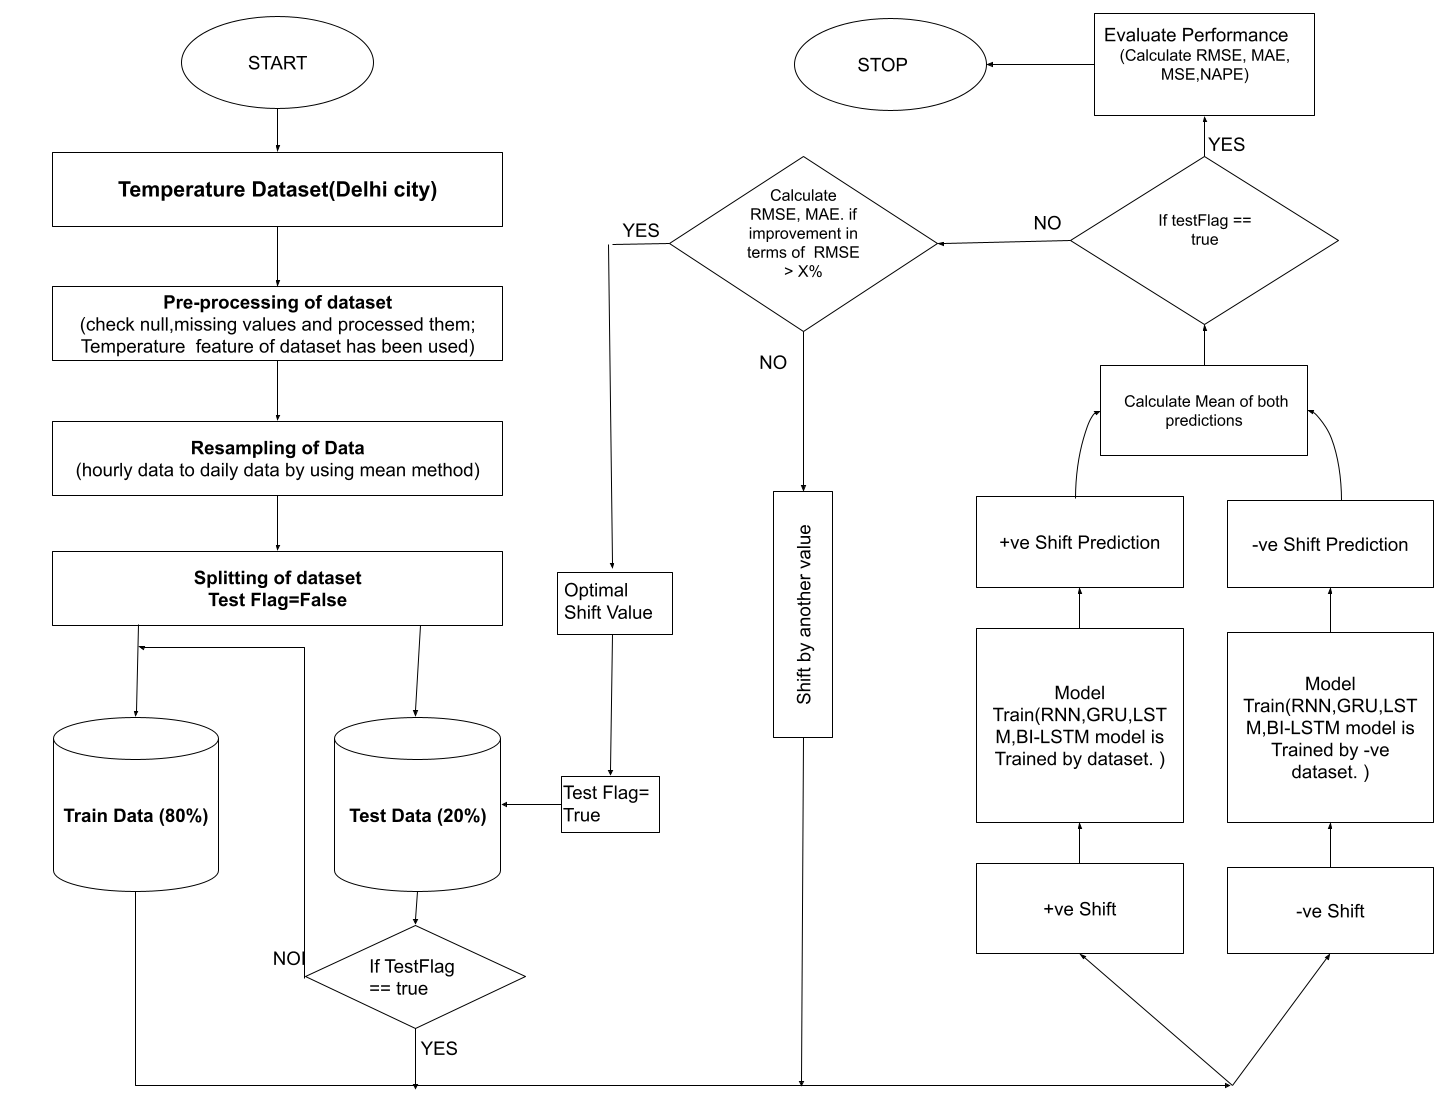
\includegraphics[width=1\textwidth, height=0.9\linewidth]{FlowchartOfjournal.png}
    \caption{Flowchart Of Proposed Work}
    \label{fig:Flowchart Of Proposed Work}
\end{figure}
\section{Methodology}


\subsection{Steps of the Proposed model}
\par {\textbf{Step 1}: The Dataset:}\\ Collected delhi weather temperature dataset D, shown in equation \ref{eqn:d}.

\begin{equation}
\label{eqn:d}
D=\left \{ x_i, y_i \right \}_{i=1}^{k}
\end{equation}

Where D is denoted as Dataset, \(X_i\) is a Temperature data of 10 min. interval, and \(Y_i\) its corresponding time. k denotes the number of samples in the Dataset. For all \(Y_i\) belongs to Y.

\par {\textbf{Step 2}: Resizing of the Dataset:}\\ dataset D has been resized into a new dimension. The function representing the dimension is omega. shown in equation \ref{eqn:c}.

\begin{equation}
\label{eqn:c}
D_{new}=\omega \left ( D, p  \times q \right )
\end{equation}

Where \(D_{new}\) is the preprocessed the dataset D. Here,  p x q  are the new dimension of the Dataset.

\par {\textbf{Step 3}: Splitting Dataset:}\\ The preprocessed Dataset has been divided into three parts: training \((T_{train})\), testing \((T_{test})\), and validation \((V_{valid})\). The Dataset is mutually exclusive in equation \ref{eqn:a} and exhaustive in equation \ref{eqn:b}.

\begin{equation}
\label{eqn:a}
D_{Tr}\cup D_{Te}=D_{T}
\end{equation}

\begin{equation}
\label{eqn:b}
\left \{ D_{Tr} \cap D_{Te} \right \}=\varnothing 
\end{equation}

\par {\textbf{Step 4}: Applying Deep Learning Models:}\\ the model \(\emptyset\left(D_{Tr}\ ,\ D_{Te}\right)\) has been applied. In the model's training and test part, the forecasting has been obtained for the test sample. Prediction is obtained:\(\left\{P_i^\emptyset\right\}_i^m\),  where m is number of test sample %\cite{hrithik2022classification}.

\par {\textbf{Step 5}: Root Mean Squared Error:}\\ RMSE is calculated by equation \ref{eqn:e}.



Where N is total no of test Sample, \(\hat{y_{i}}\) is a predicted data of model, and \(y_{i}\) is the actual test deta.\\
\par {\textbf{Step 6}: Proposed Technique:} \\
For the data points $x_i$in the training dataset $D_{Tr}$, two series can be created as in equation \ref{eqn:01}:
\begin{equation}
\begin{aligned}
\label{eqn:01}
\{x_i^{\prime}=x_i+s\}_{i=1}^n \\
\{x_i^{\prime\prime}=x_i-s\}_{i=1}^n \; \forall x_i \in D_{Tr}
\end{aligned}
\end{equation}
where $s \in Z$ and $x_i^{\prime}$ and $x_{i}^{\prime\prime}$ depicts the positive and negative series obtained by shifting the series with positive and negative values of the step length $s$ of the shift. The series have been prepared for $n$ number of iterations.
Predictions for both the positive $x_i^{\prime}$and negative $x_i^{\prime\prime}$series has been obtained as $y_i^{\prime}$ and $y_i{\prime\prime}$ respectively.
The predictions are combined to form a final set of predictions using equation \ref{eqn:02} which is utilized for the comparison with the actual values of training dataset $D_{Tr}$
\begin{equation}
\label{eqn:02}
\hat{y}_{final}=\frac{y_i^{\prime}+y_i^{\prime\prime}}{2}
\end{equation}
where $\hat{y}_{final}$ represents the final prediction. The above procedure is repeated for $n$ number of iterations and an optimal value of $s$ is obtained for which the RMSE is best out of $n$ number of iterations. 
Then, the model is trained for the actual training data $D_{Tr}$ and predictions are obtained for the test data $D_{Te}$ which is $D_{Te}^{\prime}$. Further two positive and negative series are obtained from test prediction $D_{Te}^{\prime}$ as reflected in equation \ref{eqn:03}.
\begin{equation}
\begin{aligned}
\label{eqn:03}
\{x_j^{\prime}=x_j+s\} \\
\{x_j^{\prime\prime}=x_j-s\} \; \forall x_j \in D_{Te}^{\prime}
\end{aligned}
\end{equation}
where $s$ is the step length obtained earlier and $x_j^{\prime}$ and $x_{j}^{\prime\prime}$ depicts the positive and negative series obtained by shifting the series with positive and negative values of the step length $s$ of the test predictions $ D_{Te}^{\prime}$.
Predictions for both the positive $x_j^{\prime}$and negative $x_j^{\prime\prime}$series has been obtained as $y_j^{\prime}$ and $y_j{\prime\prime}$ respectively.

The predictions are combined to form a final set of predictions using equation \ref{eqn:04} which is utilized for the comparison with the actual values of training dataset $D_{Te}$
\begin{equation}
\label{eqn:04}
\hat{y}_{final}^{\prime}=\frac{y_j^{\prime}+y_j^{\prime\prime}}{2}
\end{equation}
where $\hat{y}_{final}^{\prime}$ represents the final prediction.
\subsection{Implamentation setup and parameters settings}
The various packages of Python are utilised to implement the baseline models and  proposed models. These include Pandas (v1.5.3), Scikit-Learn (v1.2.2) for model creation and performance analysis, Keras (v2.12.0), TensorFlow (v2.12.0) for Keras backend, and NumPy (v1.23.5) for exploratory data analysis,  and For describing the findings and creating graphs, we used Plotly (v5.14.1), seaborn (v0.12.2), and matplotlib (v3.7.1). In order to create flowcharts, it has also used \href{https: //app.diagrams.net/}{https: //app.diagrams.net/} . One systems were employed for the experiments:  a MacOS-based computer with Apple M1 having 8 GB RAM. and all exprement done on Google colab having runtime type Python 3 and hardware accelerate T4 GPU with 12.7Gb Ram.

\begin{table*}[h!]
  \caption{Parameter setting of traditional DL models and proposed Models}
  \label{tab: my-table}
  \begin{tabular}{ll}
  \hline Hyperparameters & Values        \\ \hline
  Batch Size               & 32                     \\
  Optimizer                 & Adam                   \\
  Loss function            & Mean Squared Error      \\
  Epoch                    & 200 with early stopping \\
  training size             & 0.8                   \\ \hline
  \end{tabular}
  \end{table*}

\section{Results and discussion}\label{sec2}
The percentage improvement  of the experimented models namely LSTM, GRU, BiLSTM and RNN has been depicted in Table \ref{tab:MSE} on the basis of MSE. The maximum improvement achieved is of 47.33 \% in case of GRU where the shift length is kept as 35. Other models also show significant improvement after the implementation of proposed methodology.
% \begin{table}[ht!]
% \centering
% \caption{MSE}
% \label{tab:MSE}
% \begin{tabular}{lllll}
% \hline
% \textbf{MODELS} & \textbf{ORIGINAL} & \textbf{\% IMPROVEMENT} & \textbf{PROPOSED (P)} & \textbf{SHIFT LENGTH} \\ \hline
% \textbf{LSTM}    & 1.97   & 19.54 & 1.59 & 20 \\
% \textbf{GRU}     & 3.35 & 47.73 & 1.75 & 35 \\
% \textbf{BI-LSTM} & 1.62   & 15.86 & 1.36 & 35 \\
% \textbf{RNN}     & 1.94   & 21.37 & 1.52 & 35 \\ \hline
% \end{tabular}
% \end{table}

\begin{table}[ht!]
\centering
\caption{PErformance of different DL models and proposed DL models}
\label{tab:MSE}
\begin{tabular}{lllll}
\hline
\textbf{MODELS} & \textbf{MSE} & \textbf{RMSE} & \textbf{MAE} & \textbf{MAPE}  \\ \hline
  LSTM    & 1.97   & 1.39 & 1.07 & 4.33 \\
  GRU    & 3.35 & 1.78 & 1.45 & 4.53 \\
  BI-LSTM & 1.62   & 1.26 & 0.99 & 4.41 \\
  RNN     & 1.94   & 1.38 & 1.09 & 4.95 \\
\textbf{Proposed LSTM}    & \textbf{1.59}   & \textbf{1.25} & \textbf{0.95} & \textbf{4.36} \\
\textbf{Proposed GRU}     & \textbf{1.75} & \textbf{1.31} & \textbf{1.03} & \textbf{4.26} \\
\textbf{Proposed BI-LSTM} & \textbf{1.36}   & \textbf{1.16} & \textbf{0.89} & \textbf{4.13} \\
\textbf{Proposed RNN}     & \textbf{1.52}   & \textbf{1.23} & \textbf{0.97} & \textbf{4.55} \\ \hline
\end{tabular}
\end{table}


% \begin{table}[ht!]
% \centering
% \caption{MAPE}
% \label{tab:MAPE}
% \begin{tabular}{lllll}
% \hline
% \textbf{MODELS} & \textbf{ORIGINAL} & \textbf{\% IMPROVEMENT} & \textbf{PROPOSED (P)} & \textbf{SHIFT LENGTH} \\ \hline
% \textbf{LSTM}    & 4.33   & -7.78 & 4.36 & 20 \\
% \textbf{GRU}     & 4.53 & 6.10 & 4.26 & 35 \\
% \textbf{BI-LSTM} & 4.41   & 6.31 & 4.13 & 35 \\
% \textbf{RNN}     & 4.95   & 8.10 & 4.55 & 35 \\ \hline
% \end{tabular}
% \end{table}

% \begin{table}[ht!]
% \centering
% \caption{RMSE}
% \label{tab:RMSE}
% \begin{tabular}{lllll}
% \hline
% \textbf{MODELS} & \textbf{ORIGINAL} & \textbf{\% IMPROVEMENT} & \textbf{PROPOSED (P)} & \textbf{SHIFT LENGTH} \\ \hline
% \textbf{LSTM}    & 1.39 & 10.0381 & 1.2593 & 20 \\
% \textbf{GRU}     & 1.78 & 25.98   & 1.31   & 35 \\
% \textbf{BI-LSTM} & 1.26 & 7.99    & 1.16   & 35 \\
% \textbf{RNN}     & 1.38 & 10.38   & 1.2343 & 35 \\ \hline
% \end{tabular}
% \end{table}
% \begin{table}[ht!]
% \centering
% \caption{MAE}
% \label{tab:MAE}
% \begin{tabular}{lllll}
% \hline
% \textbf{MODELS} & \textbf{ORIGINAL} & \textbf{\% IMPROVEMENT} & \textbf{PROPOSED (P)} & \textbf{SHIFT LENGTH} \\ \hline
% \textbf{LSTM}    & 1.07 & 11.20 & 0.95 & 20 \\
% \textbf{GRU}     & 1.45 & 28.8  & 1.03 & 35 \\
% \textbf{BI-LSTM} & 0.99 & 10.10 & 0.89 & 35 \\
% \textbf{RNN}     & 1.09 & 11.24 & 0.97 & 35 \\ \hline
% \end{tabular}
% \end{table}
Figure \ref{fig:all_models_measures} illustrates the comparison of the all experimented models with the performance of the proposed method. 
\\
\begin{figure}[ht!]
%\centering
\subfloat[LSTM Vs Proposed LSTM] {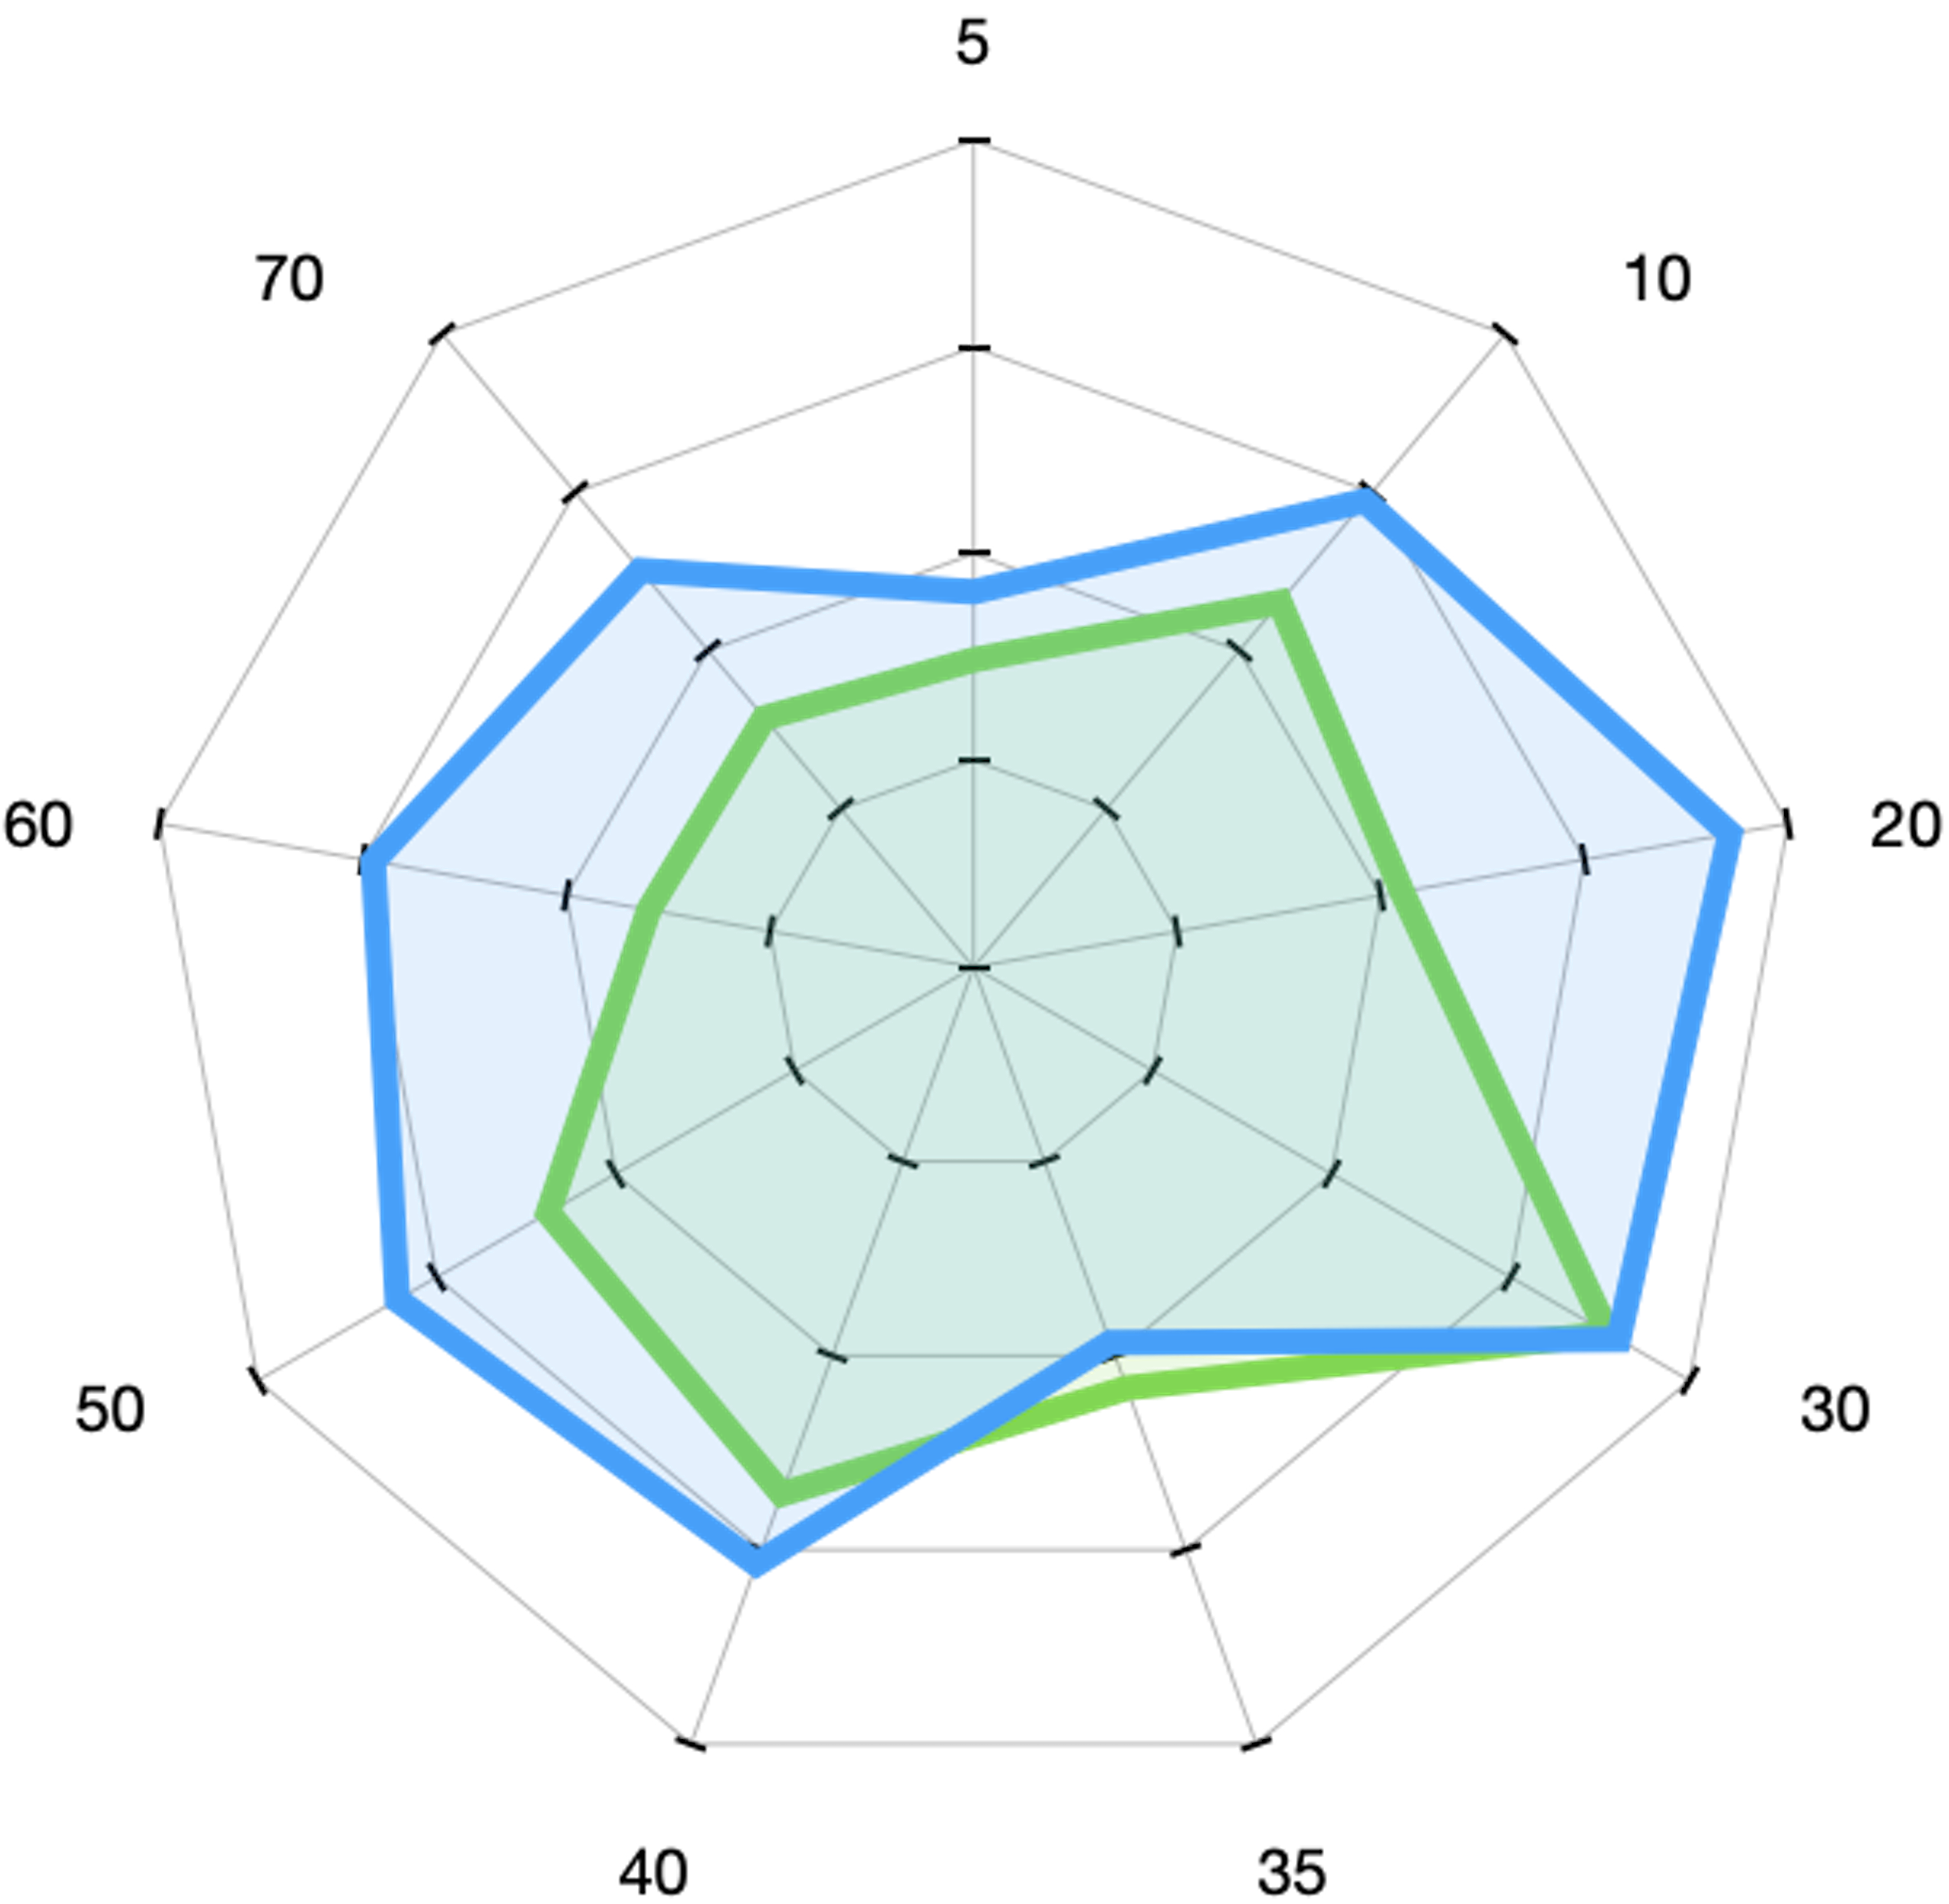
\includegraphics[width=0.4\textwidth, height=0.25\linewidth]{LSTM_MAE_SPIDER.png}\label{fig:LSTM MAE SPIDER}}
\hfill
\subfloat[RNN Vs Proposed RNN]{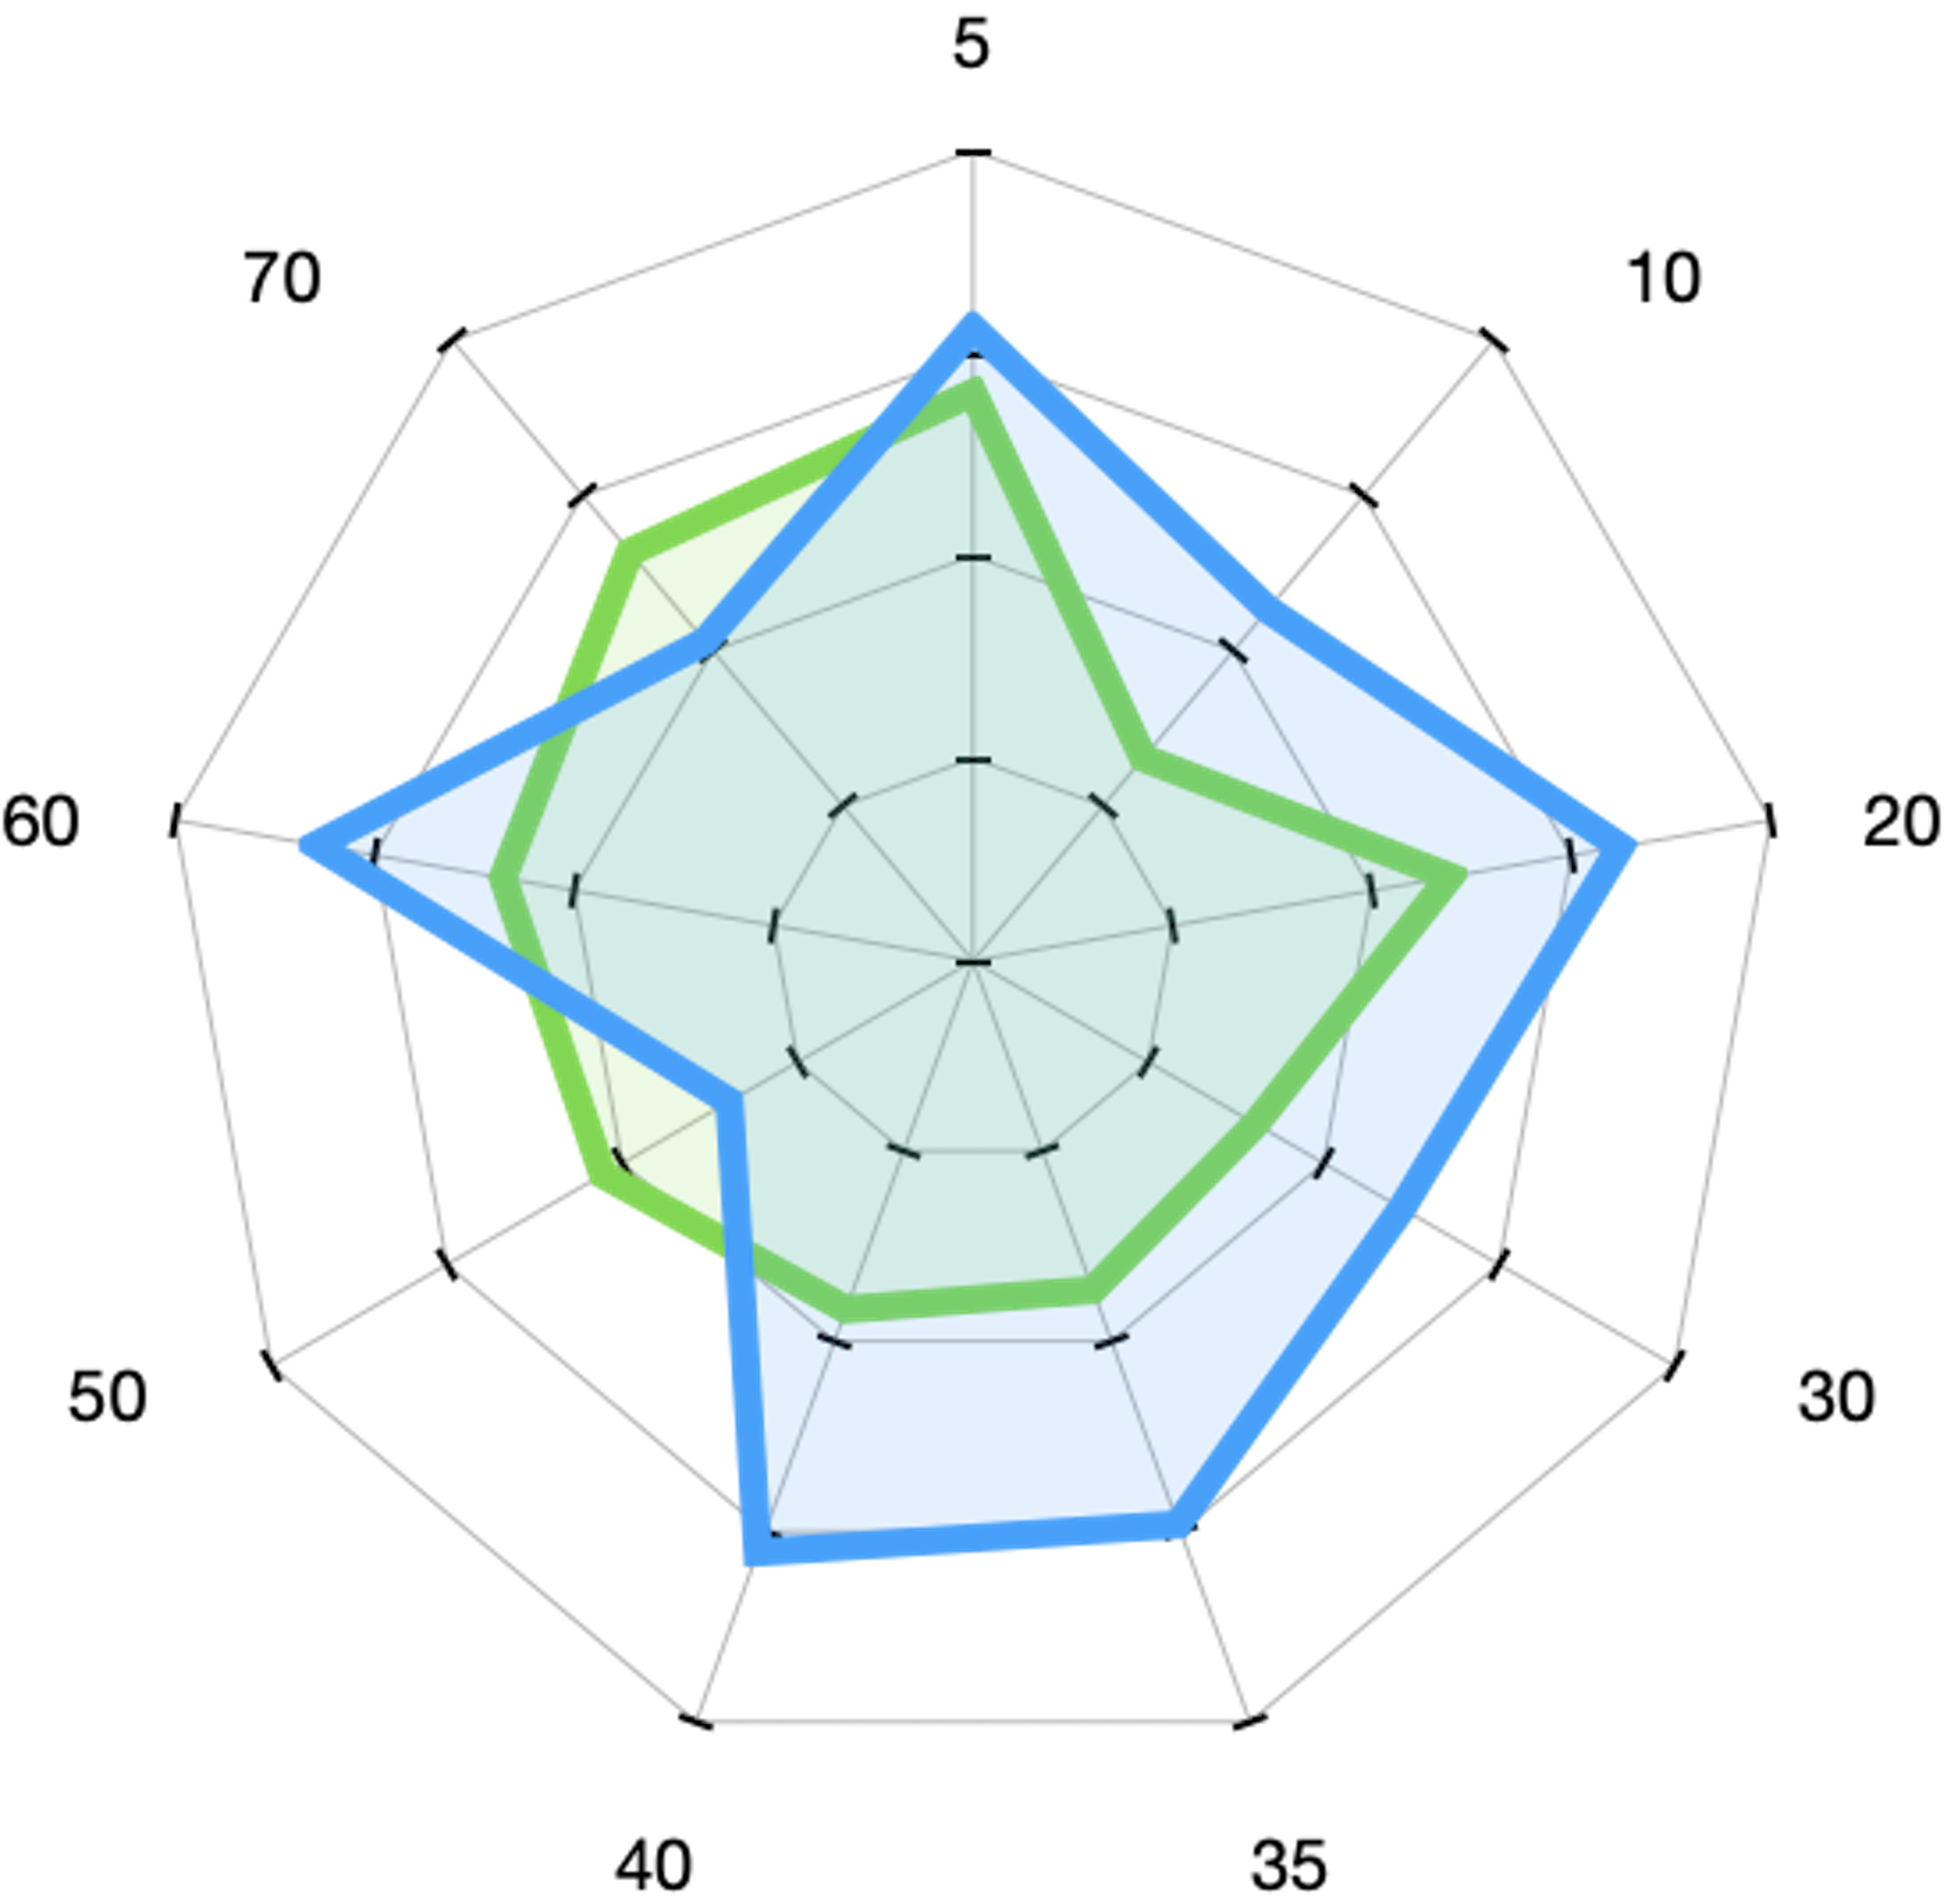
\includegraphics[width=0.4\textwidth, height=0.25\linewidth]{RNN_MAE_SPIDER.png}\label{fig:RNN_MAE_SPIDER}}\\
\subfloat[BiLSTM Vs Proposed RNN]{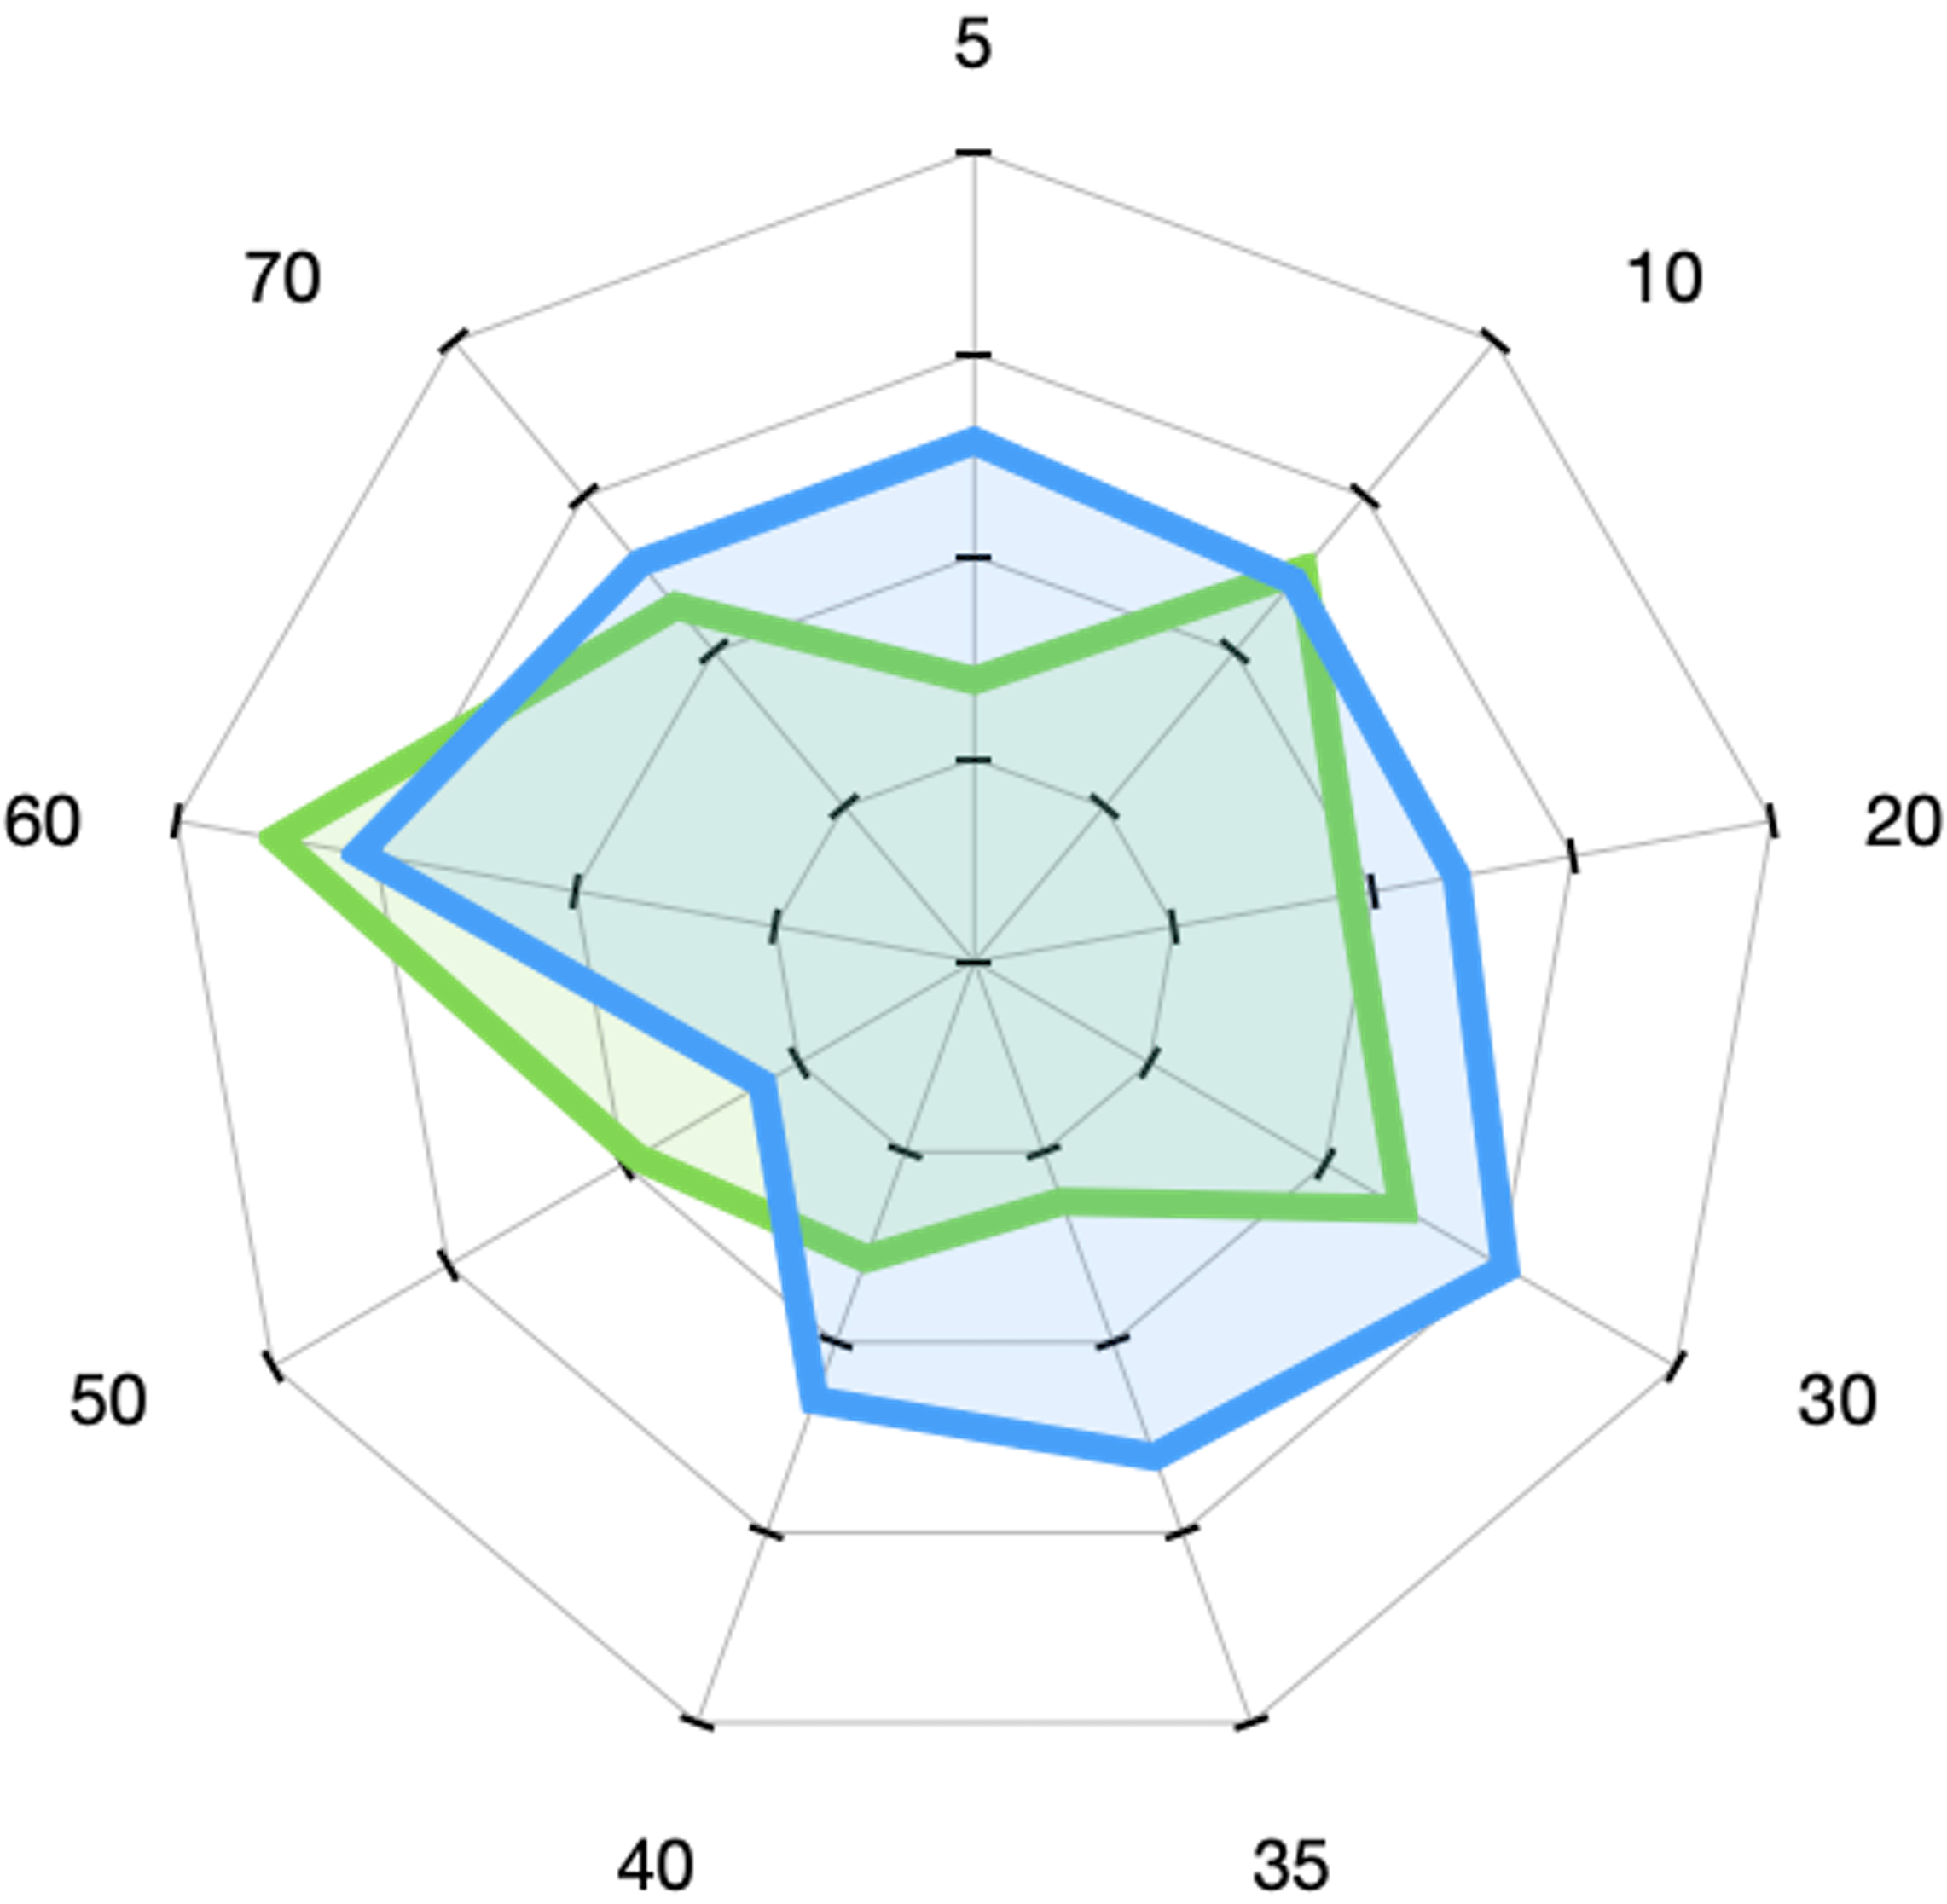
\includegraphics[width=0.4\textwidth, height=0.25\linewidth]{BI-LSTM_MAE_SPIDER.png}\label{fig:BiLSTM_MAE_SPIDER}}
\hfill
\subfloat[GRU Vs Proposed GRU]{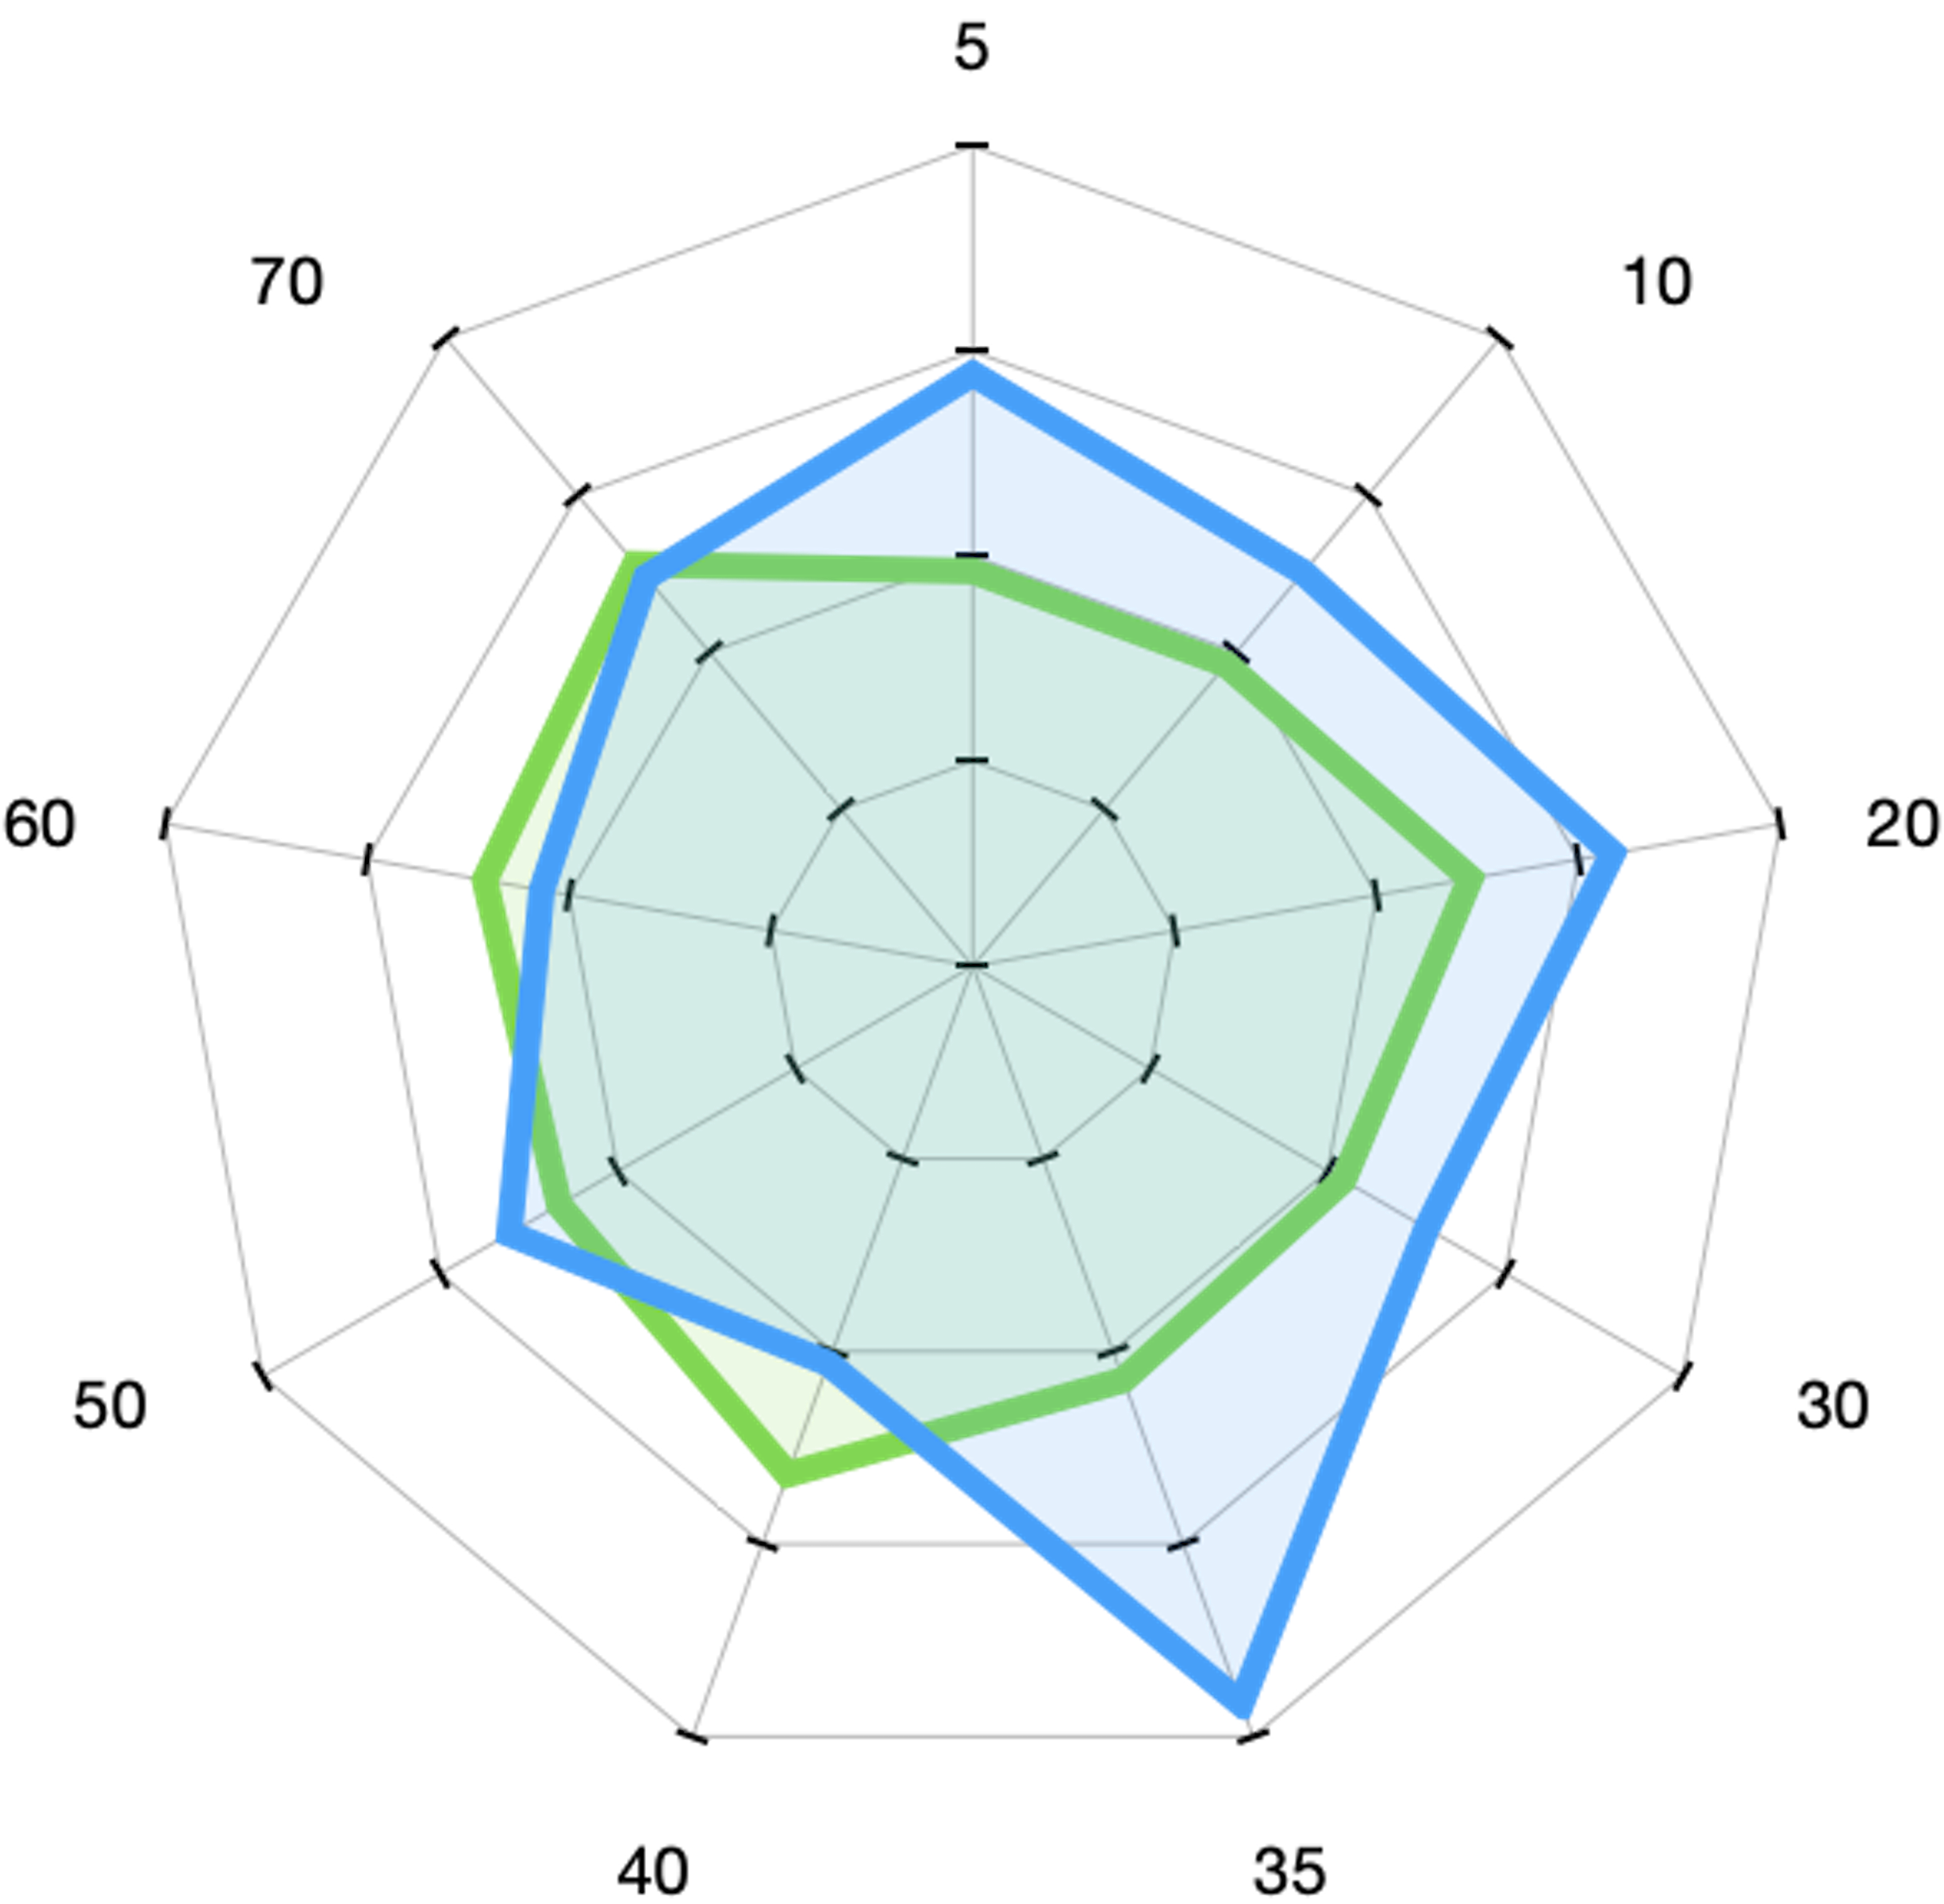
\includegraphics[width=0.4\textwidth, height=0.25\linewidth]{GRU_MAE_SPIDER.png}\label{fig:GRU_MAE_SPIDER}}
  \caption{Comparison of models over MAE}
  \label{fig:all_models_mae}
\end{figure} 
\begin{figure}[ht!]
%\centering
\subfloat[LSTM Vs Proposed LSTM]{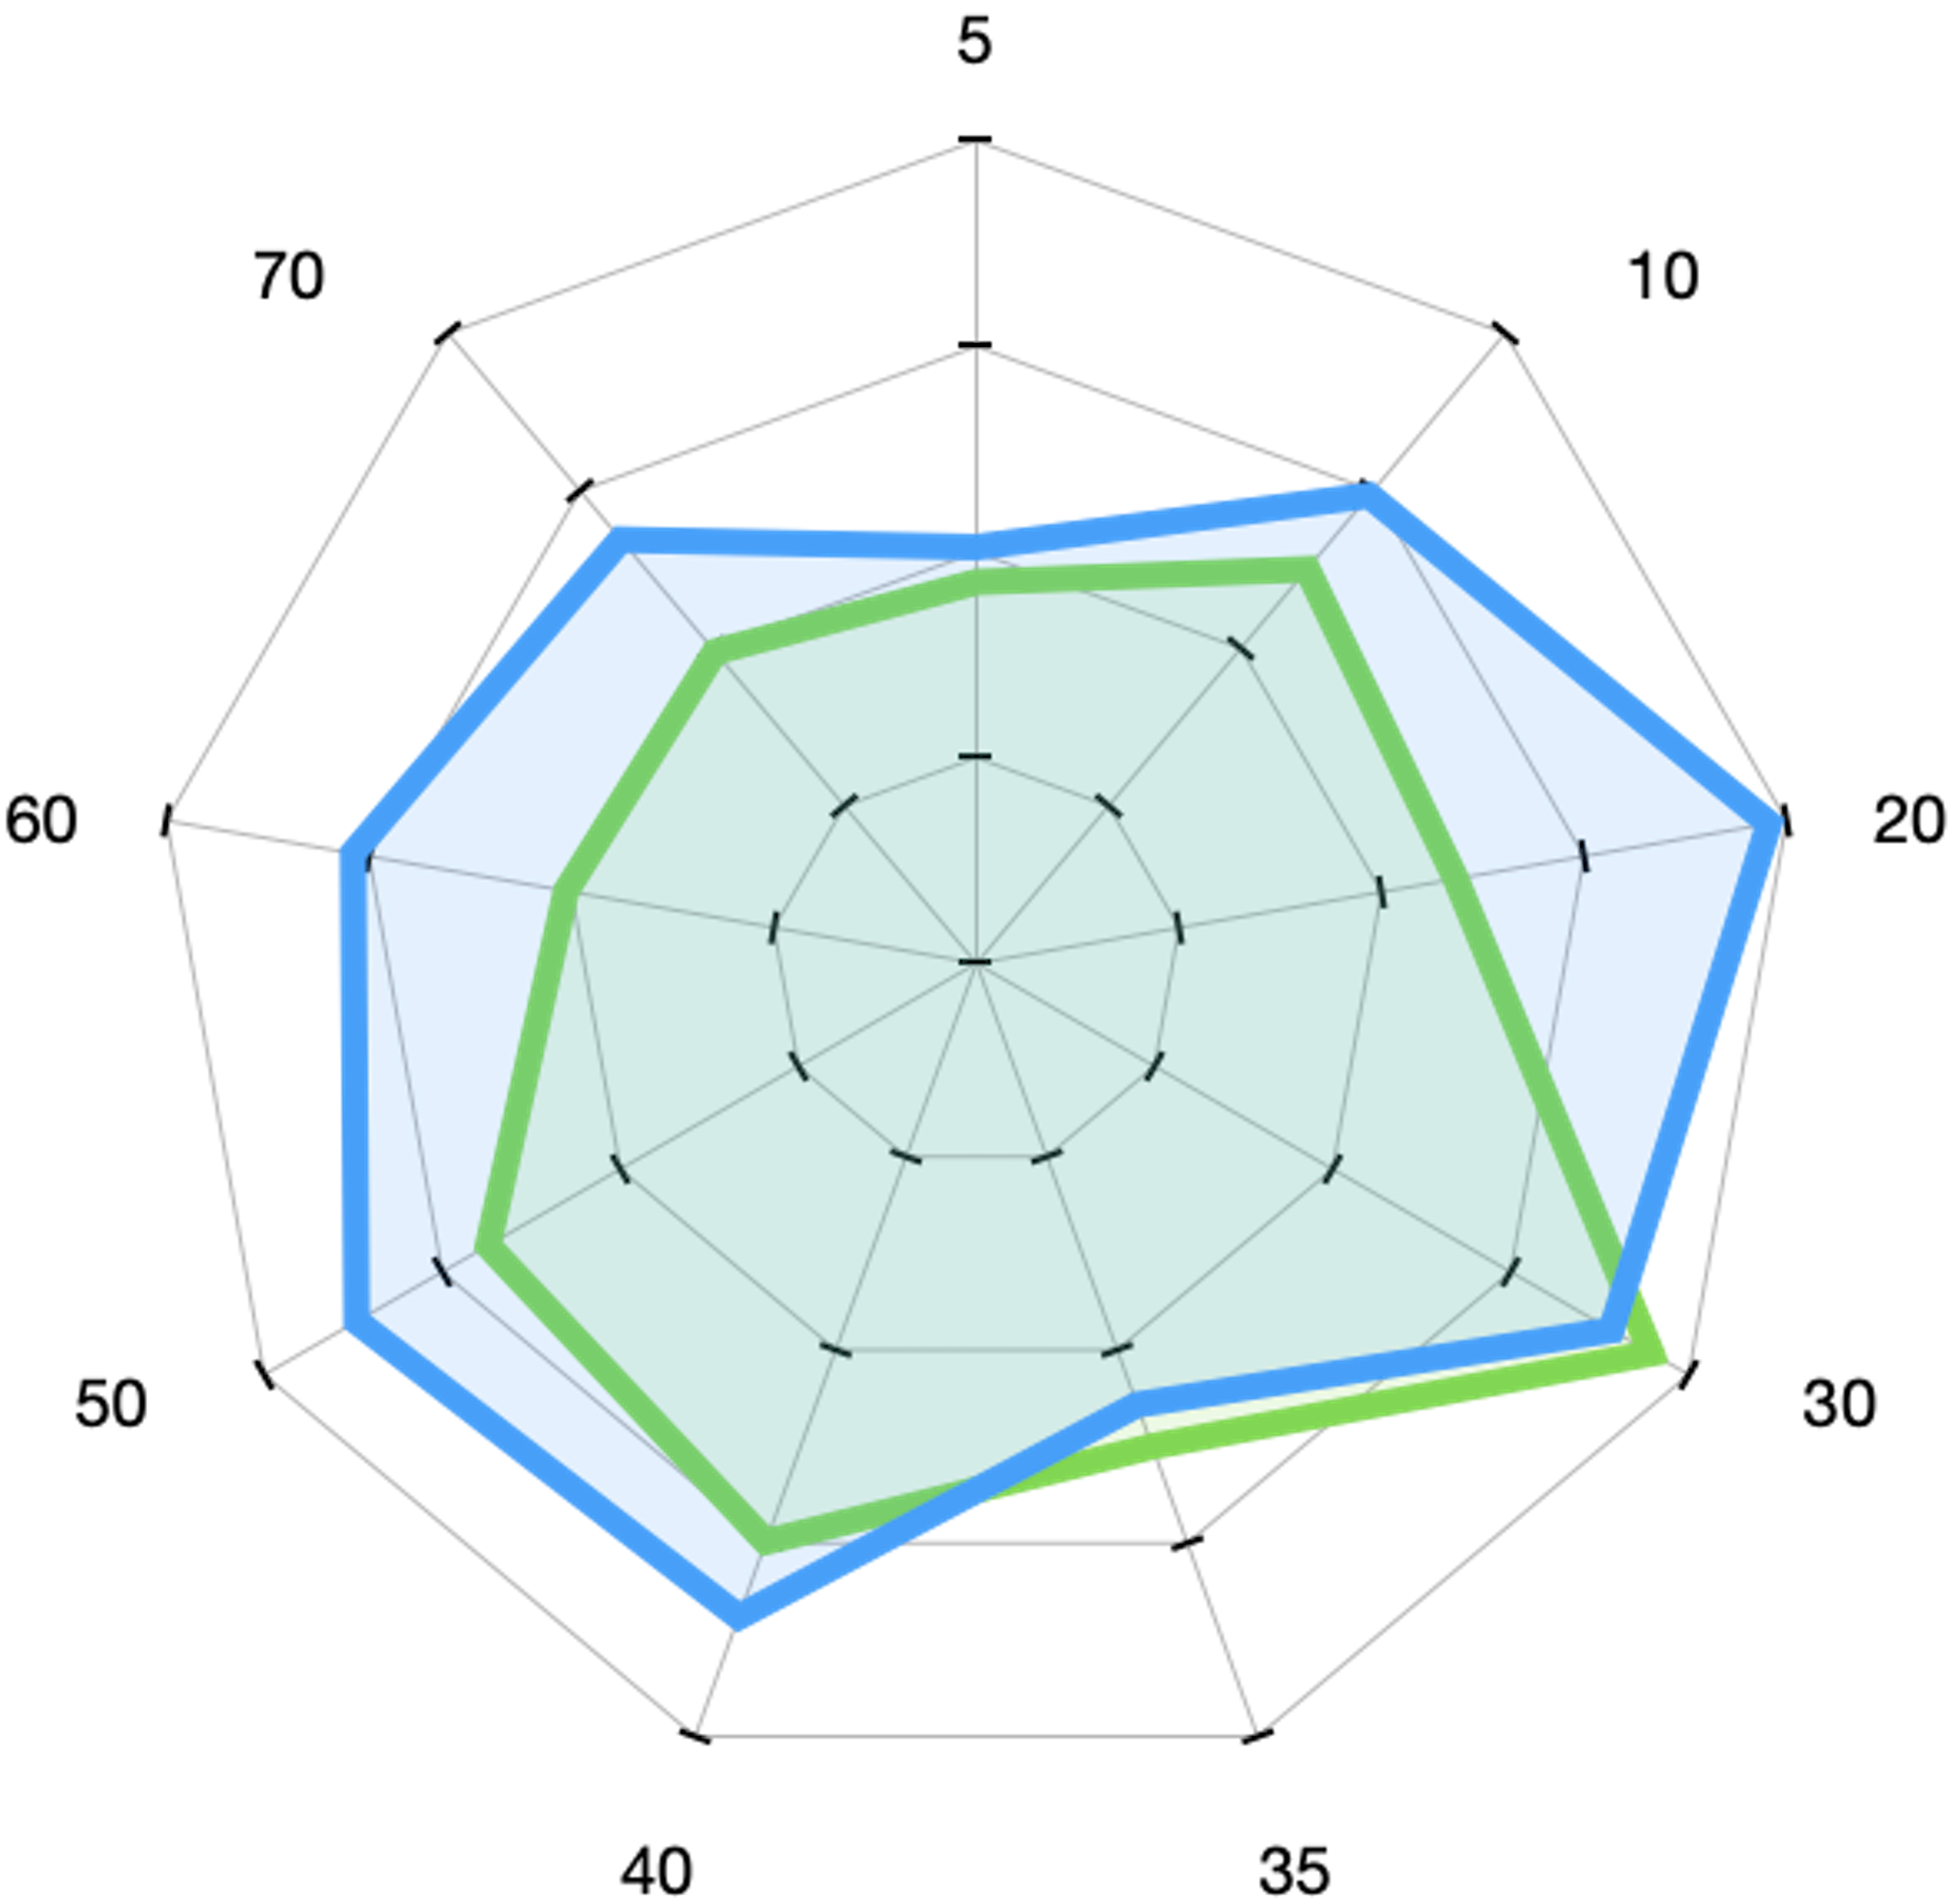
\includegraphics[width=0.4\textwidth, height=0.25\linewidth]{LSTM_MSE_SPIDER.png}\label{fig:LSTM MSE SPIDER}} 
\hfill
\subfloat[RNN Vs Proposed RNN]{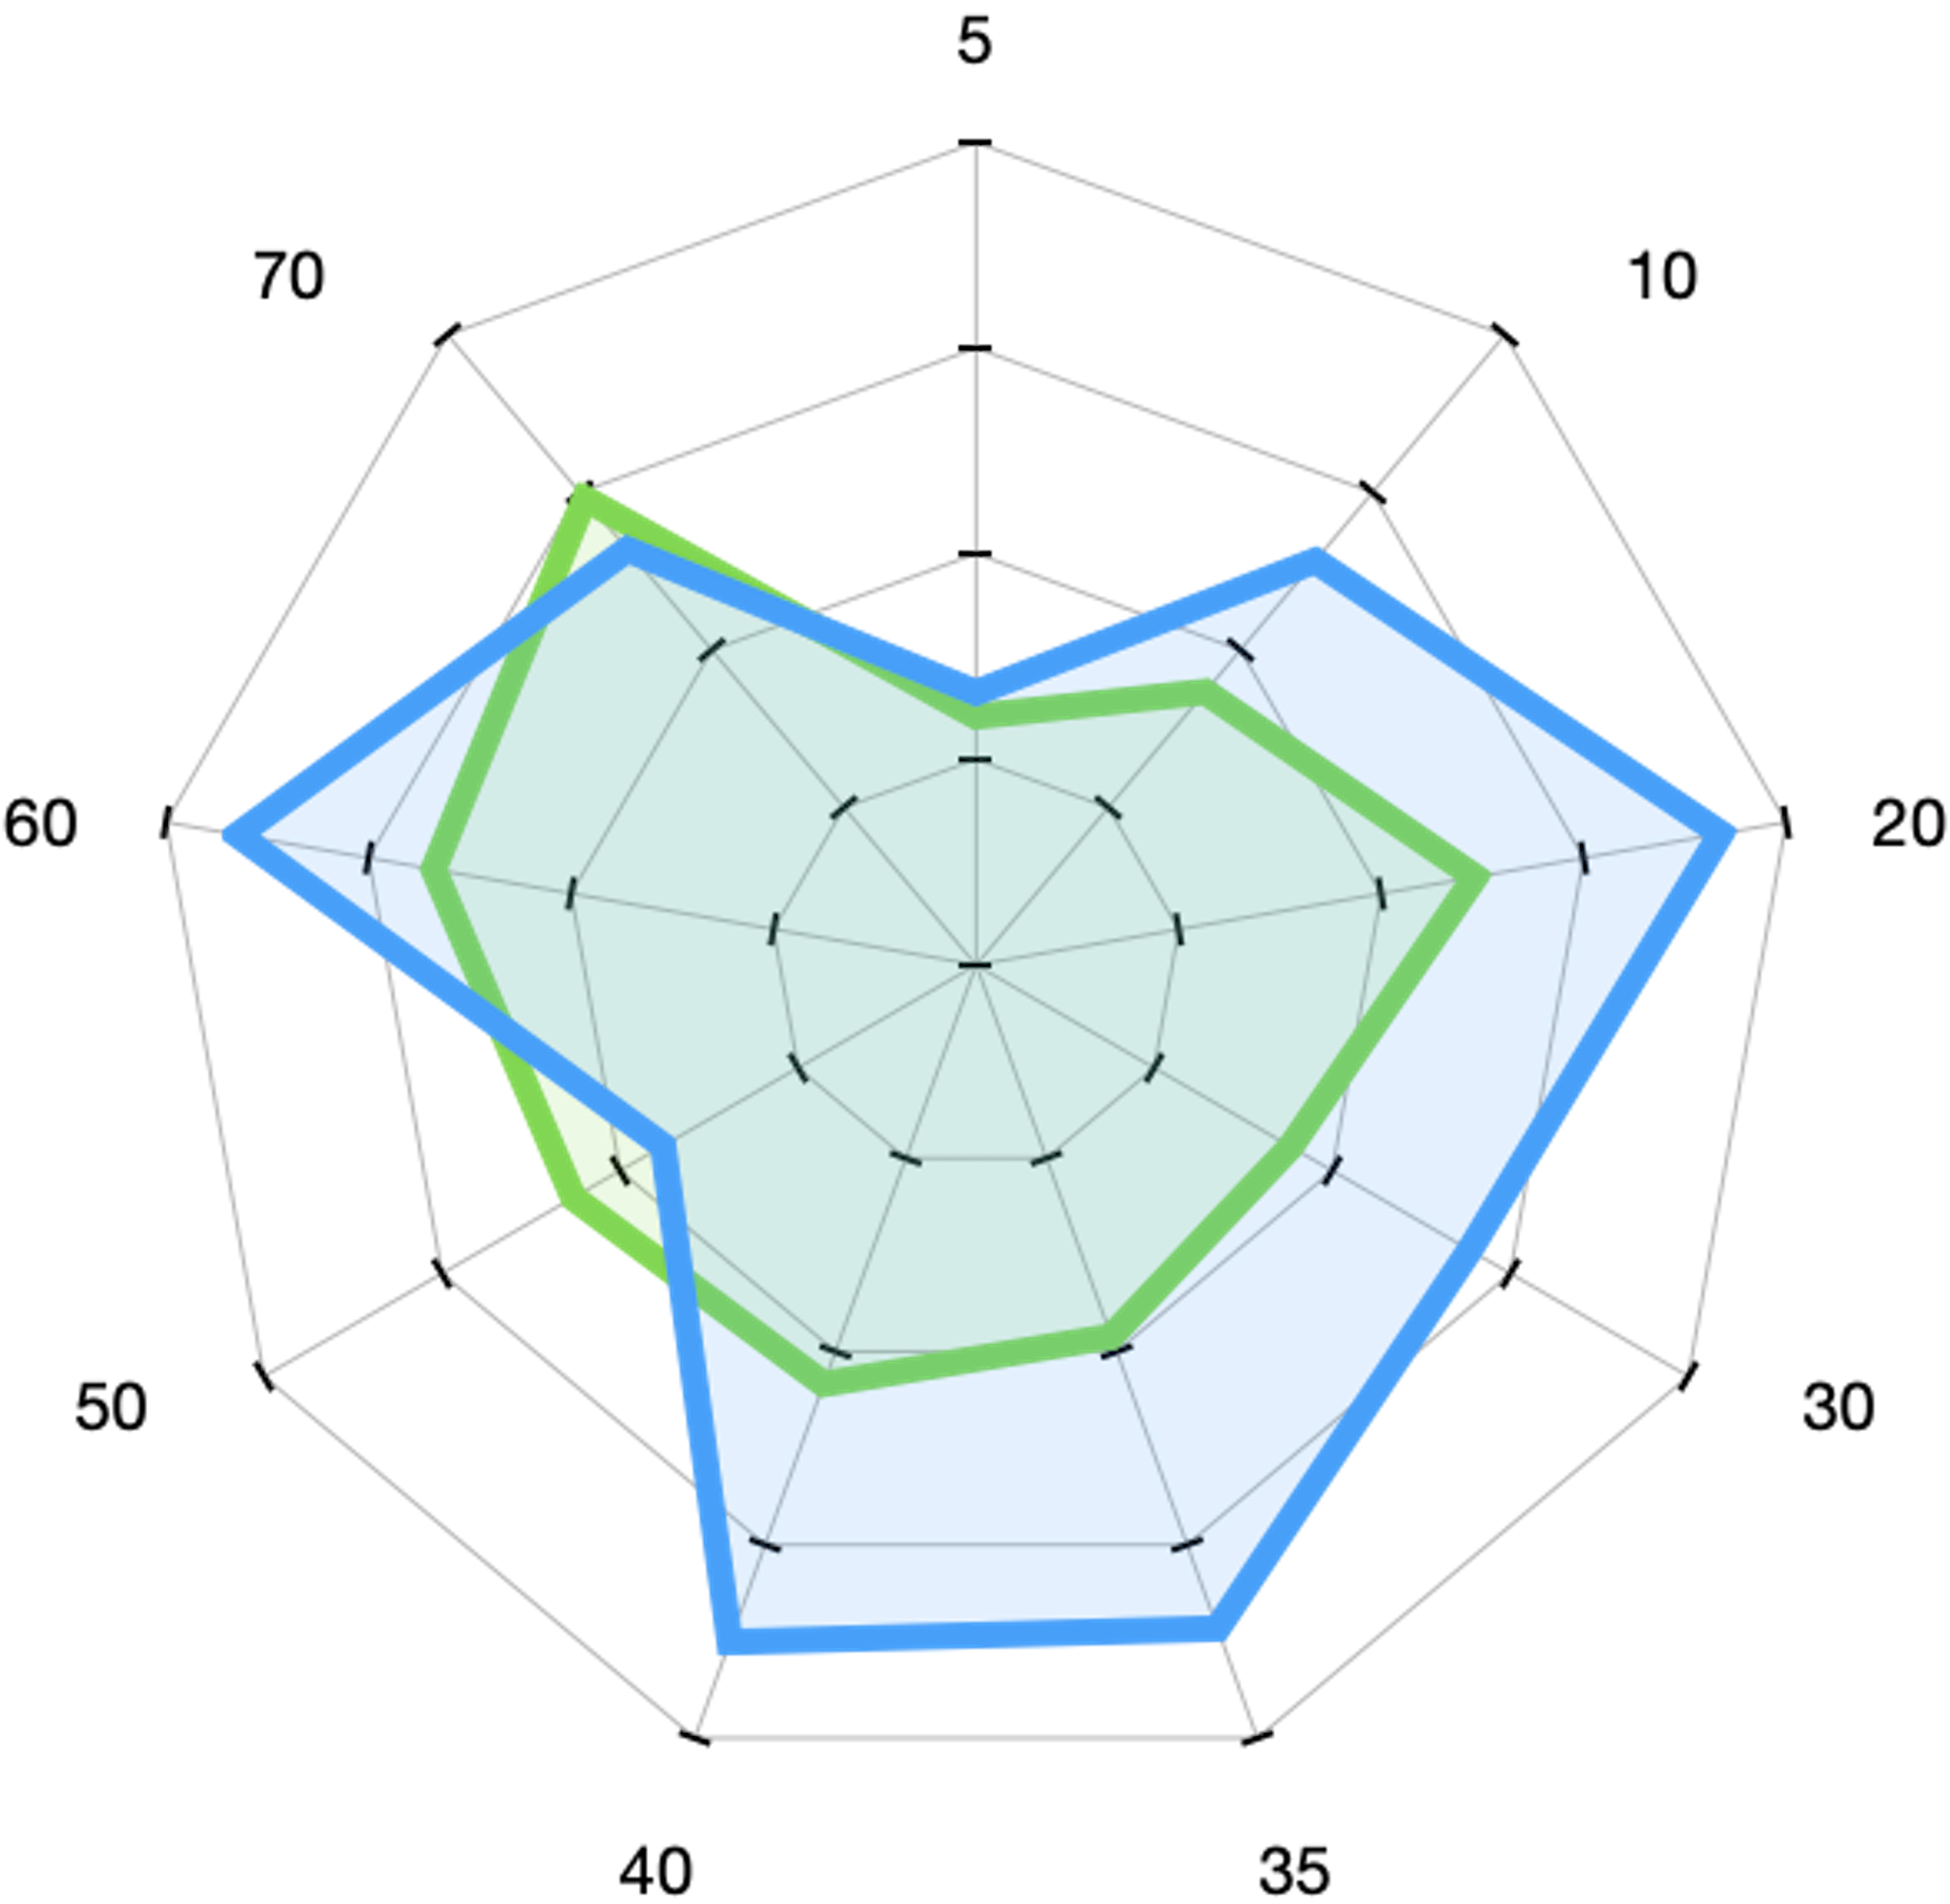
\includegraphics[width=0.4\textwidth, height=0.25\linewidth]{RNN_MSE_SPIDER.png}\label{fig:RNN_MSE_SPIDER}} 
% \vspace{\baselineskip} % Add vertical space between rows
\\
\subfloat[BiLSTM Vs Proposed RNN]{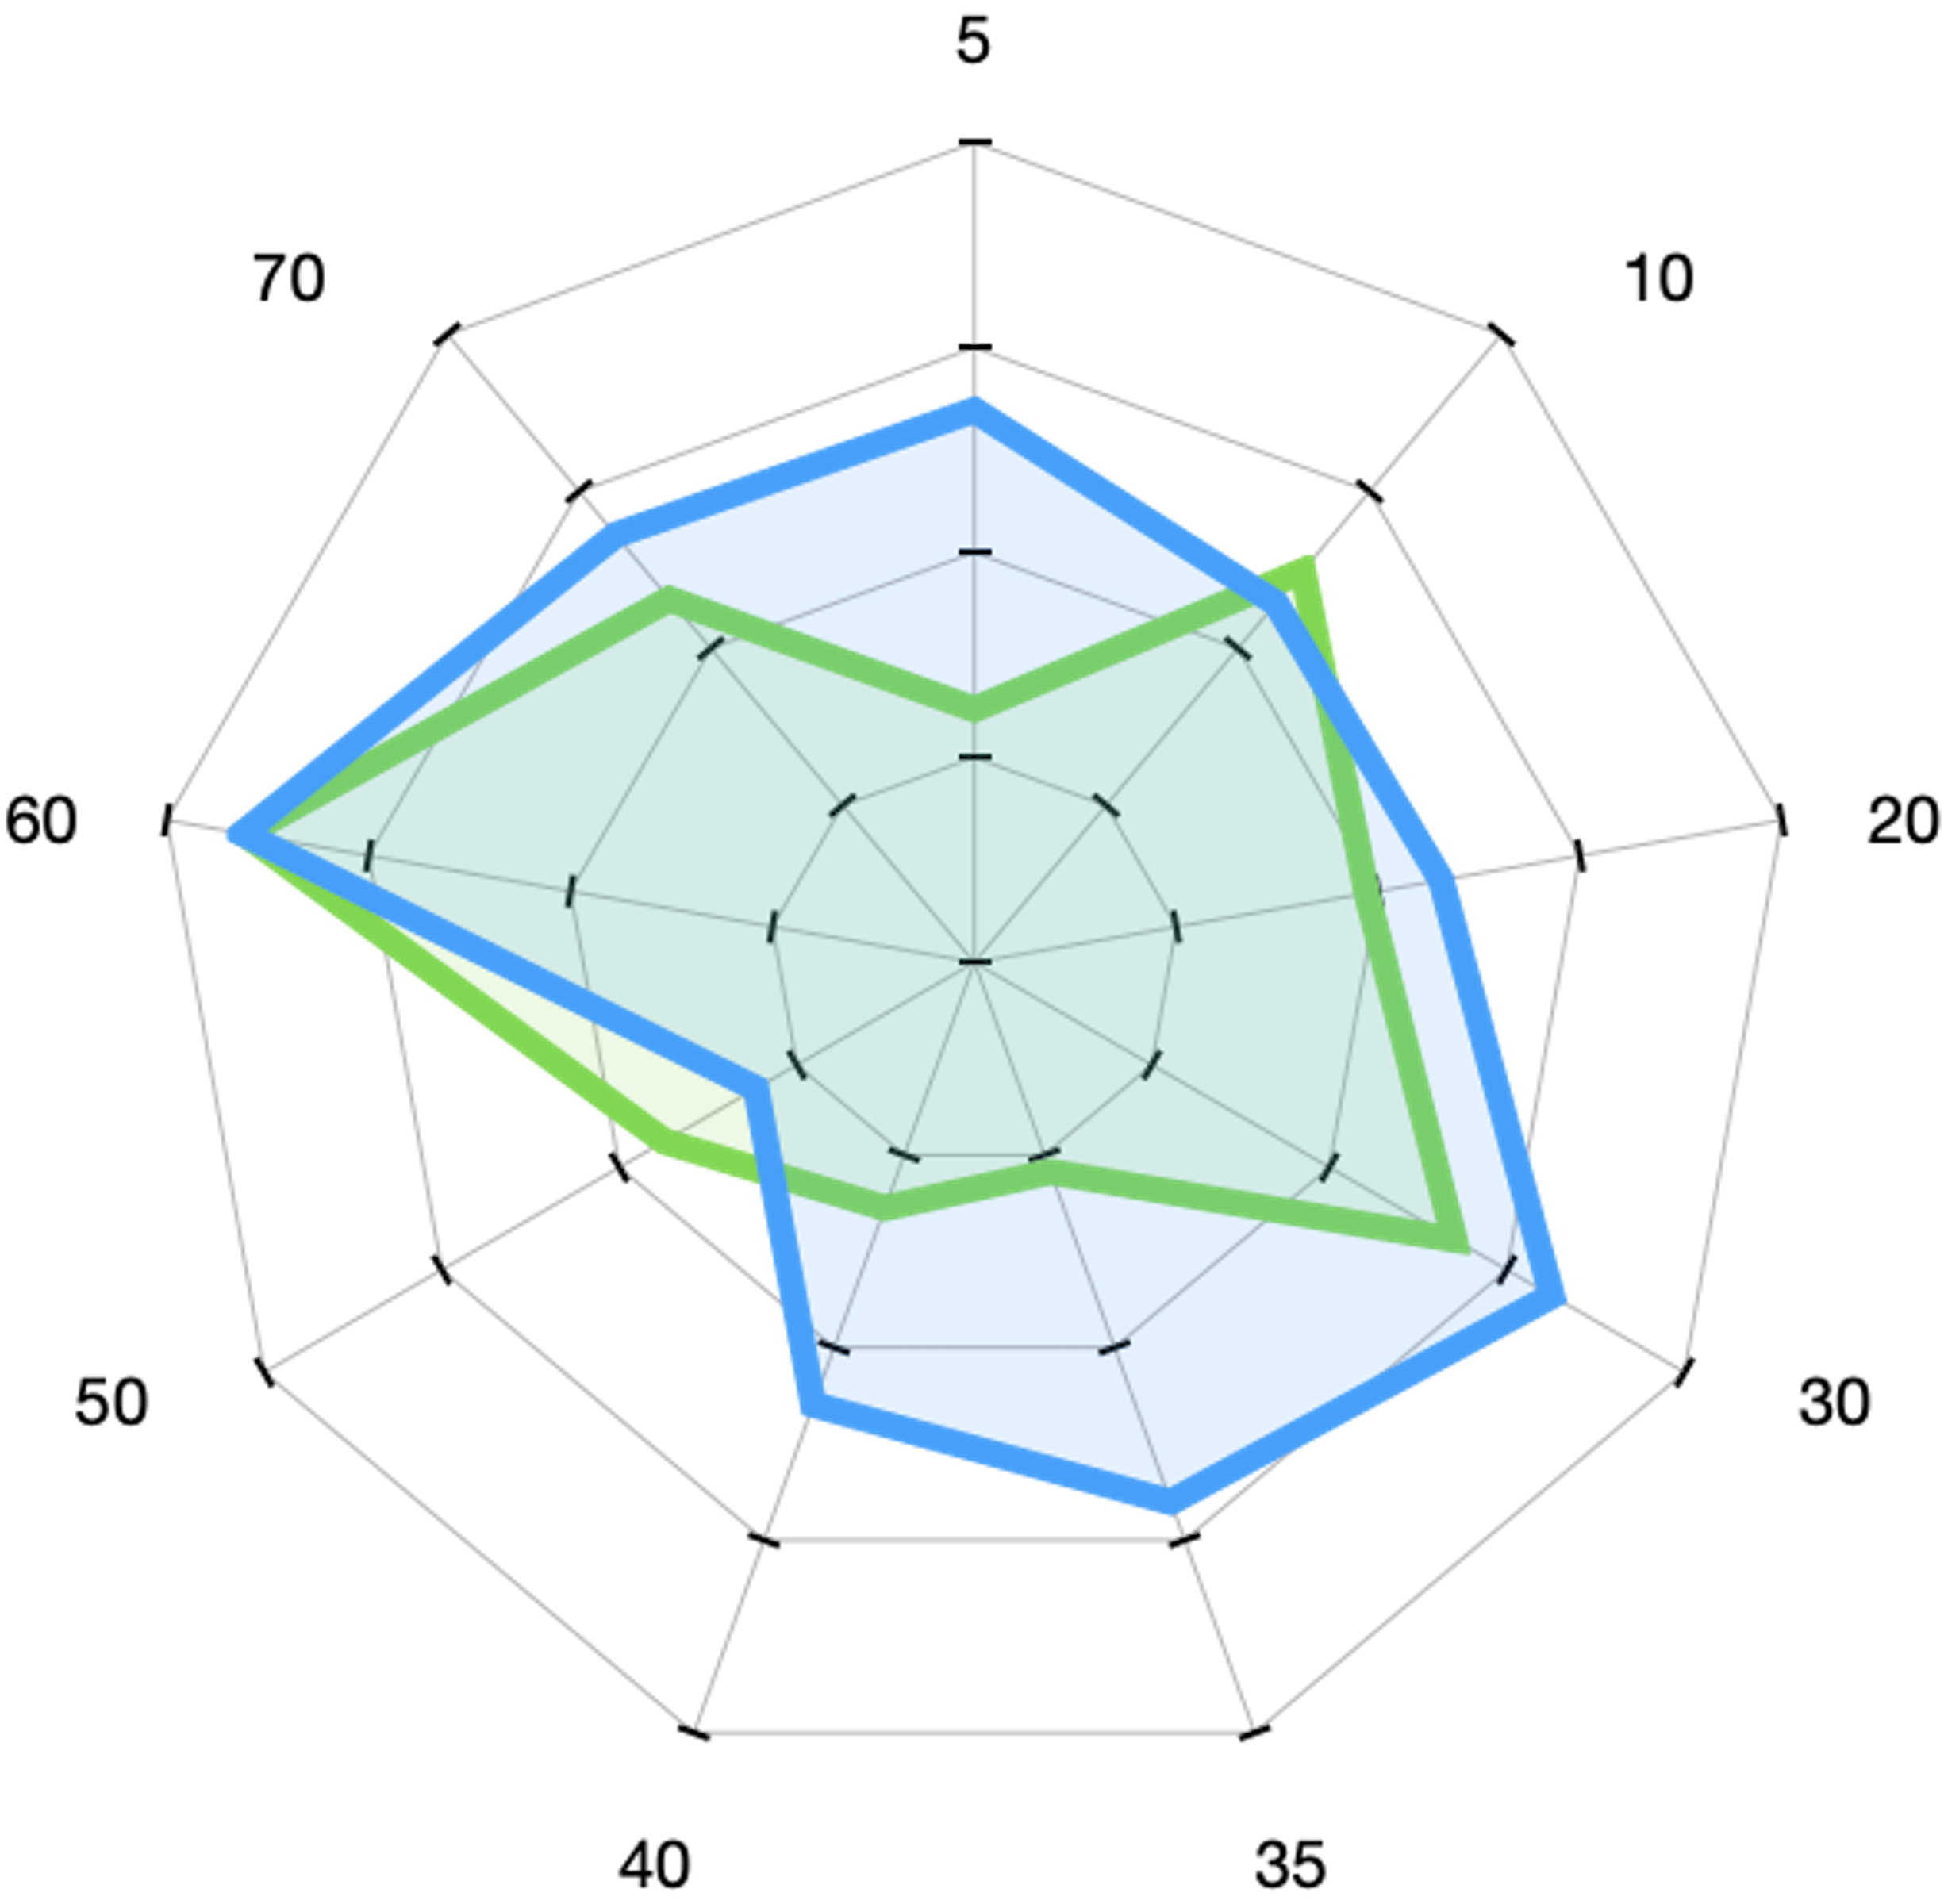
\includegraphics[width=0.4\textwidth, height=0.25\linewidth]{BI-LSTM_MSE_SPIDER.png}\label{fig:BiLSTM_MSE_SPIDER}}
\hfill
\subfloat[GRU Vs Proposed GRU]{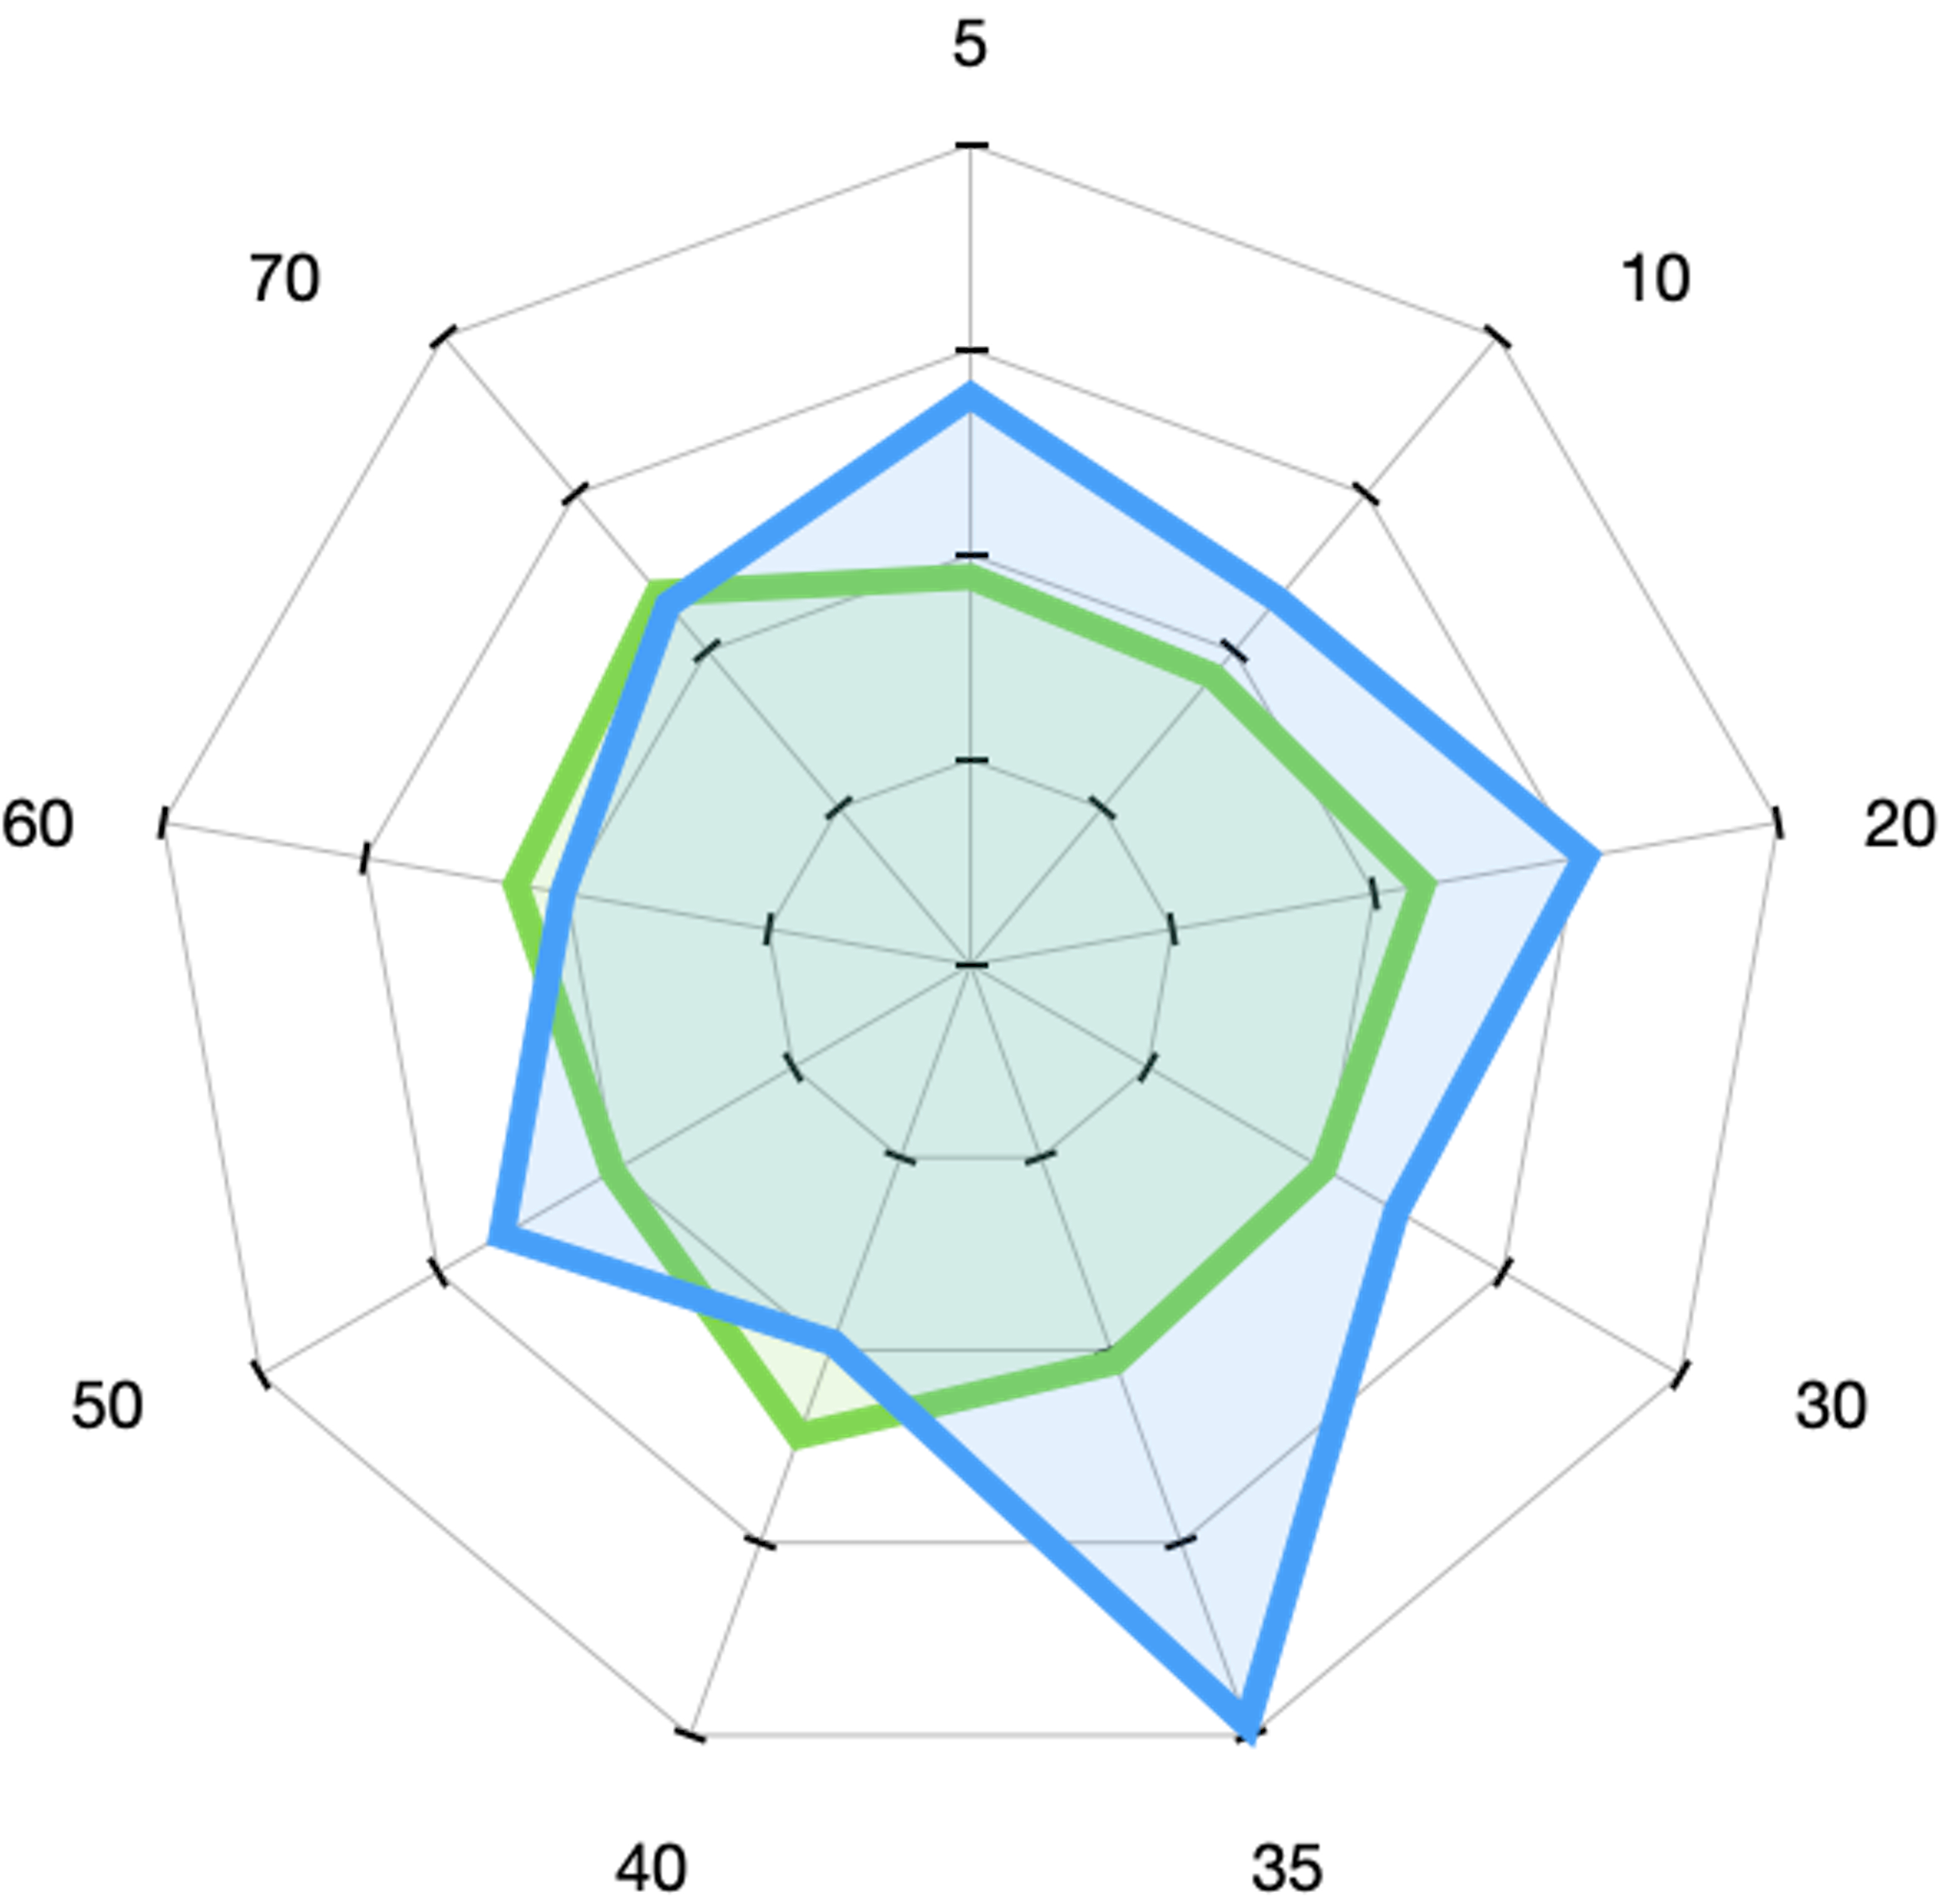
\includegraphics[width=0.4\textwidth, height=0.25\linewidth]{GRU_MSE_SPIDER.png}\label{fig:GRU_MSE_SPIDER}} 
  \caption{Comparison of models over MSE}
  \label{fig:all_models_mse}
\end{figure} 


\begin{figure}[ht!]
%\centering
\subfloat[LSTM Vs Proposed LSTM]{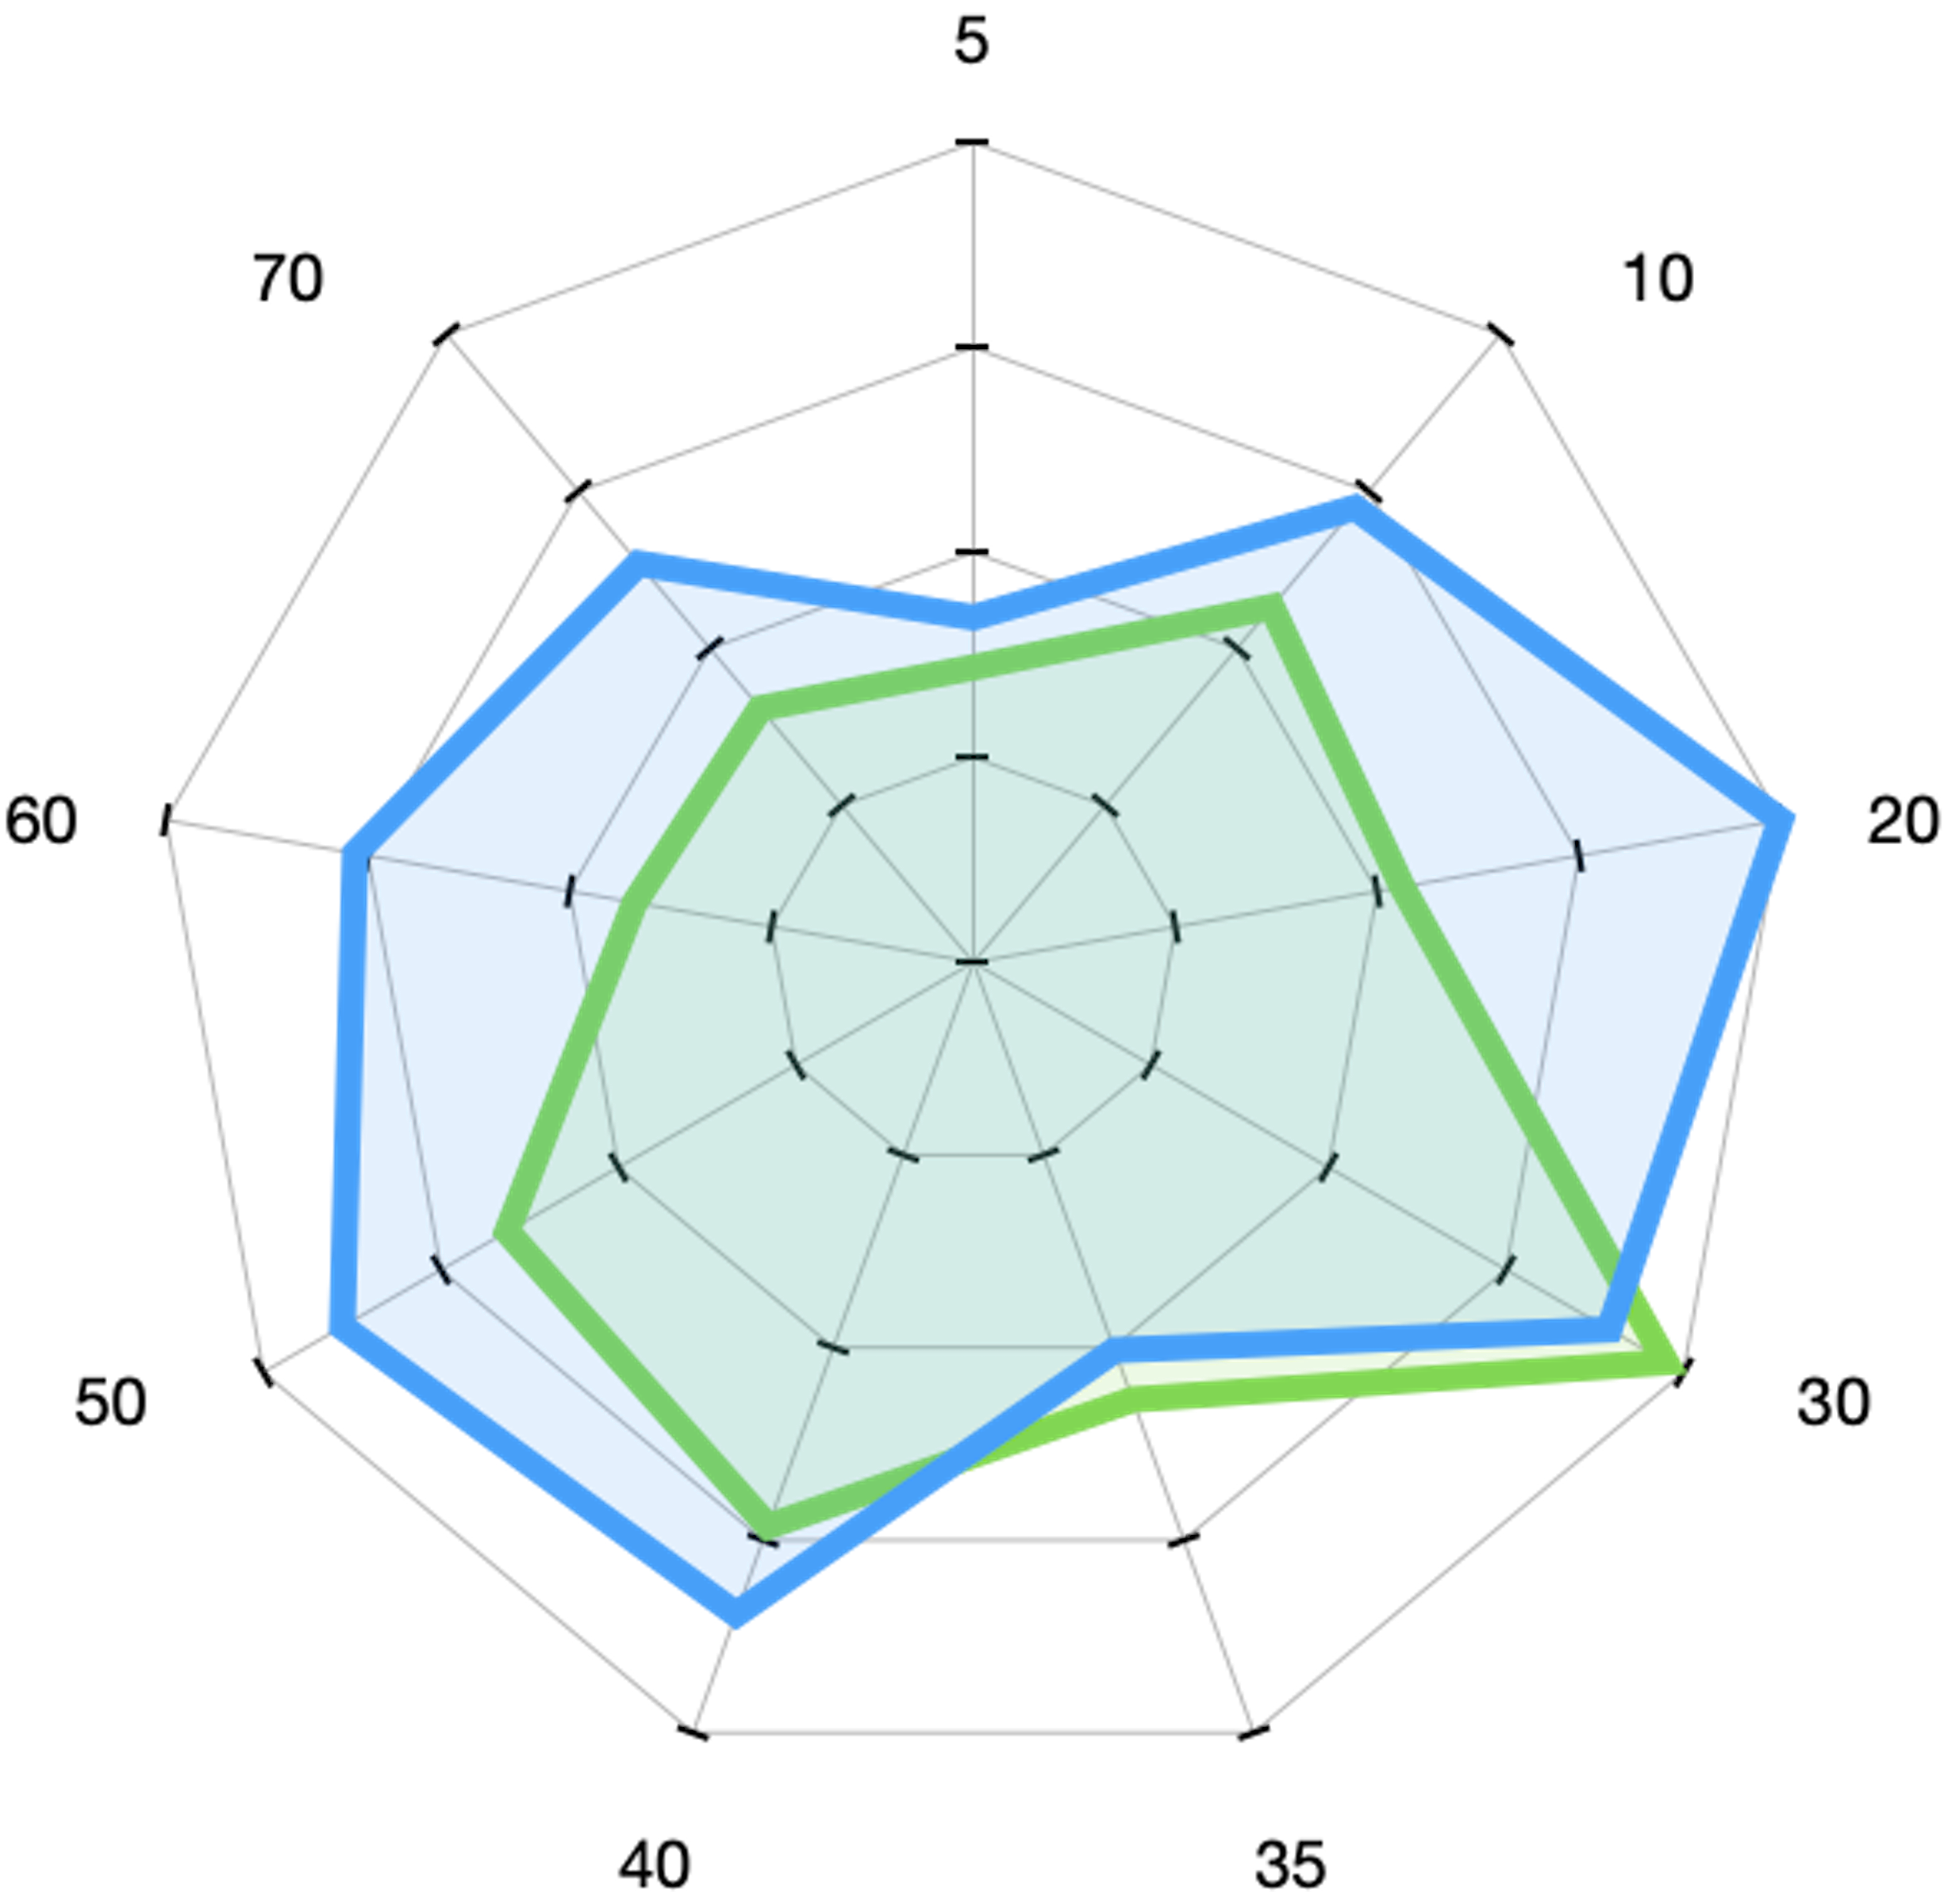
\includegraphics[width=0.4\textwidth, height=0.25\linewidth]{LSTM_RMSE_SPIDER.png}\label{fig:LSTM RMSE SPIDER}}
\hfill
\subfloat[RNN Vs Proposed RNN]{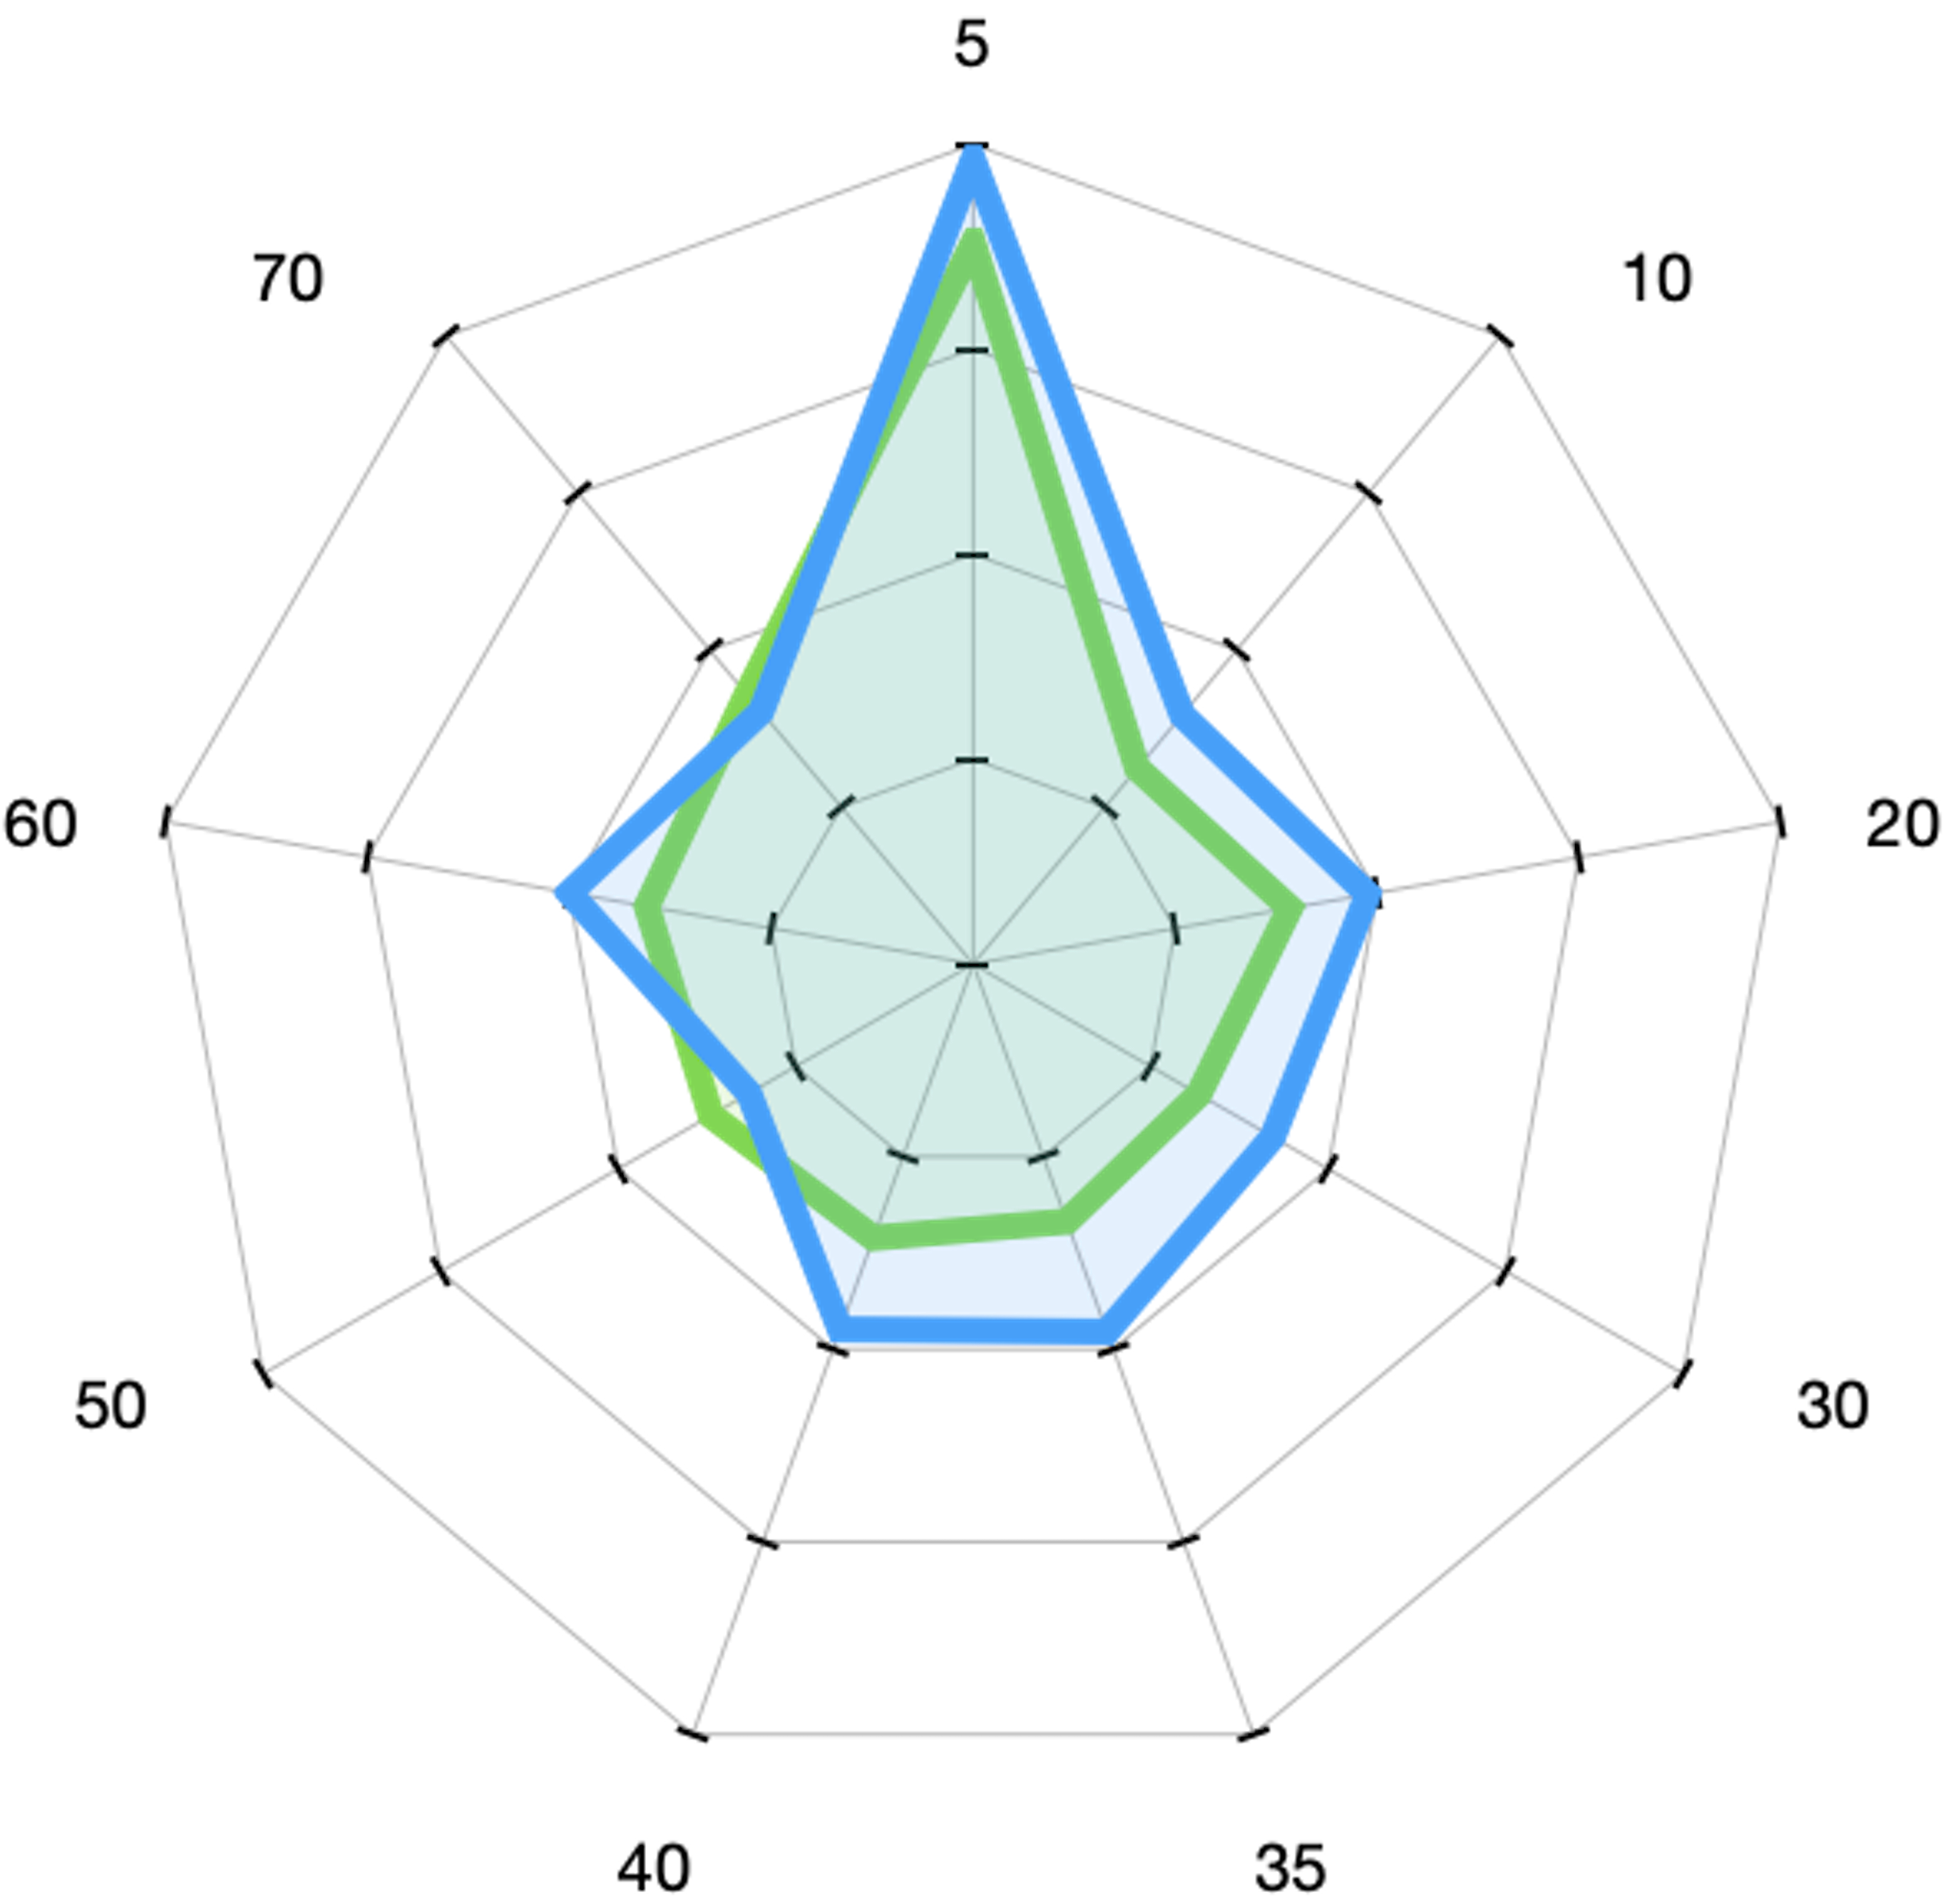
\includegraphics[width=0.4\textwidth, height=0.25\linewidth]{RNN_RMSE_SPIDER.png}\label{fig:RNN_RMSE_SPIDER}}  
\\
\subfloat[BiLSTM Vs Proposed BiLSTM]{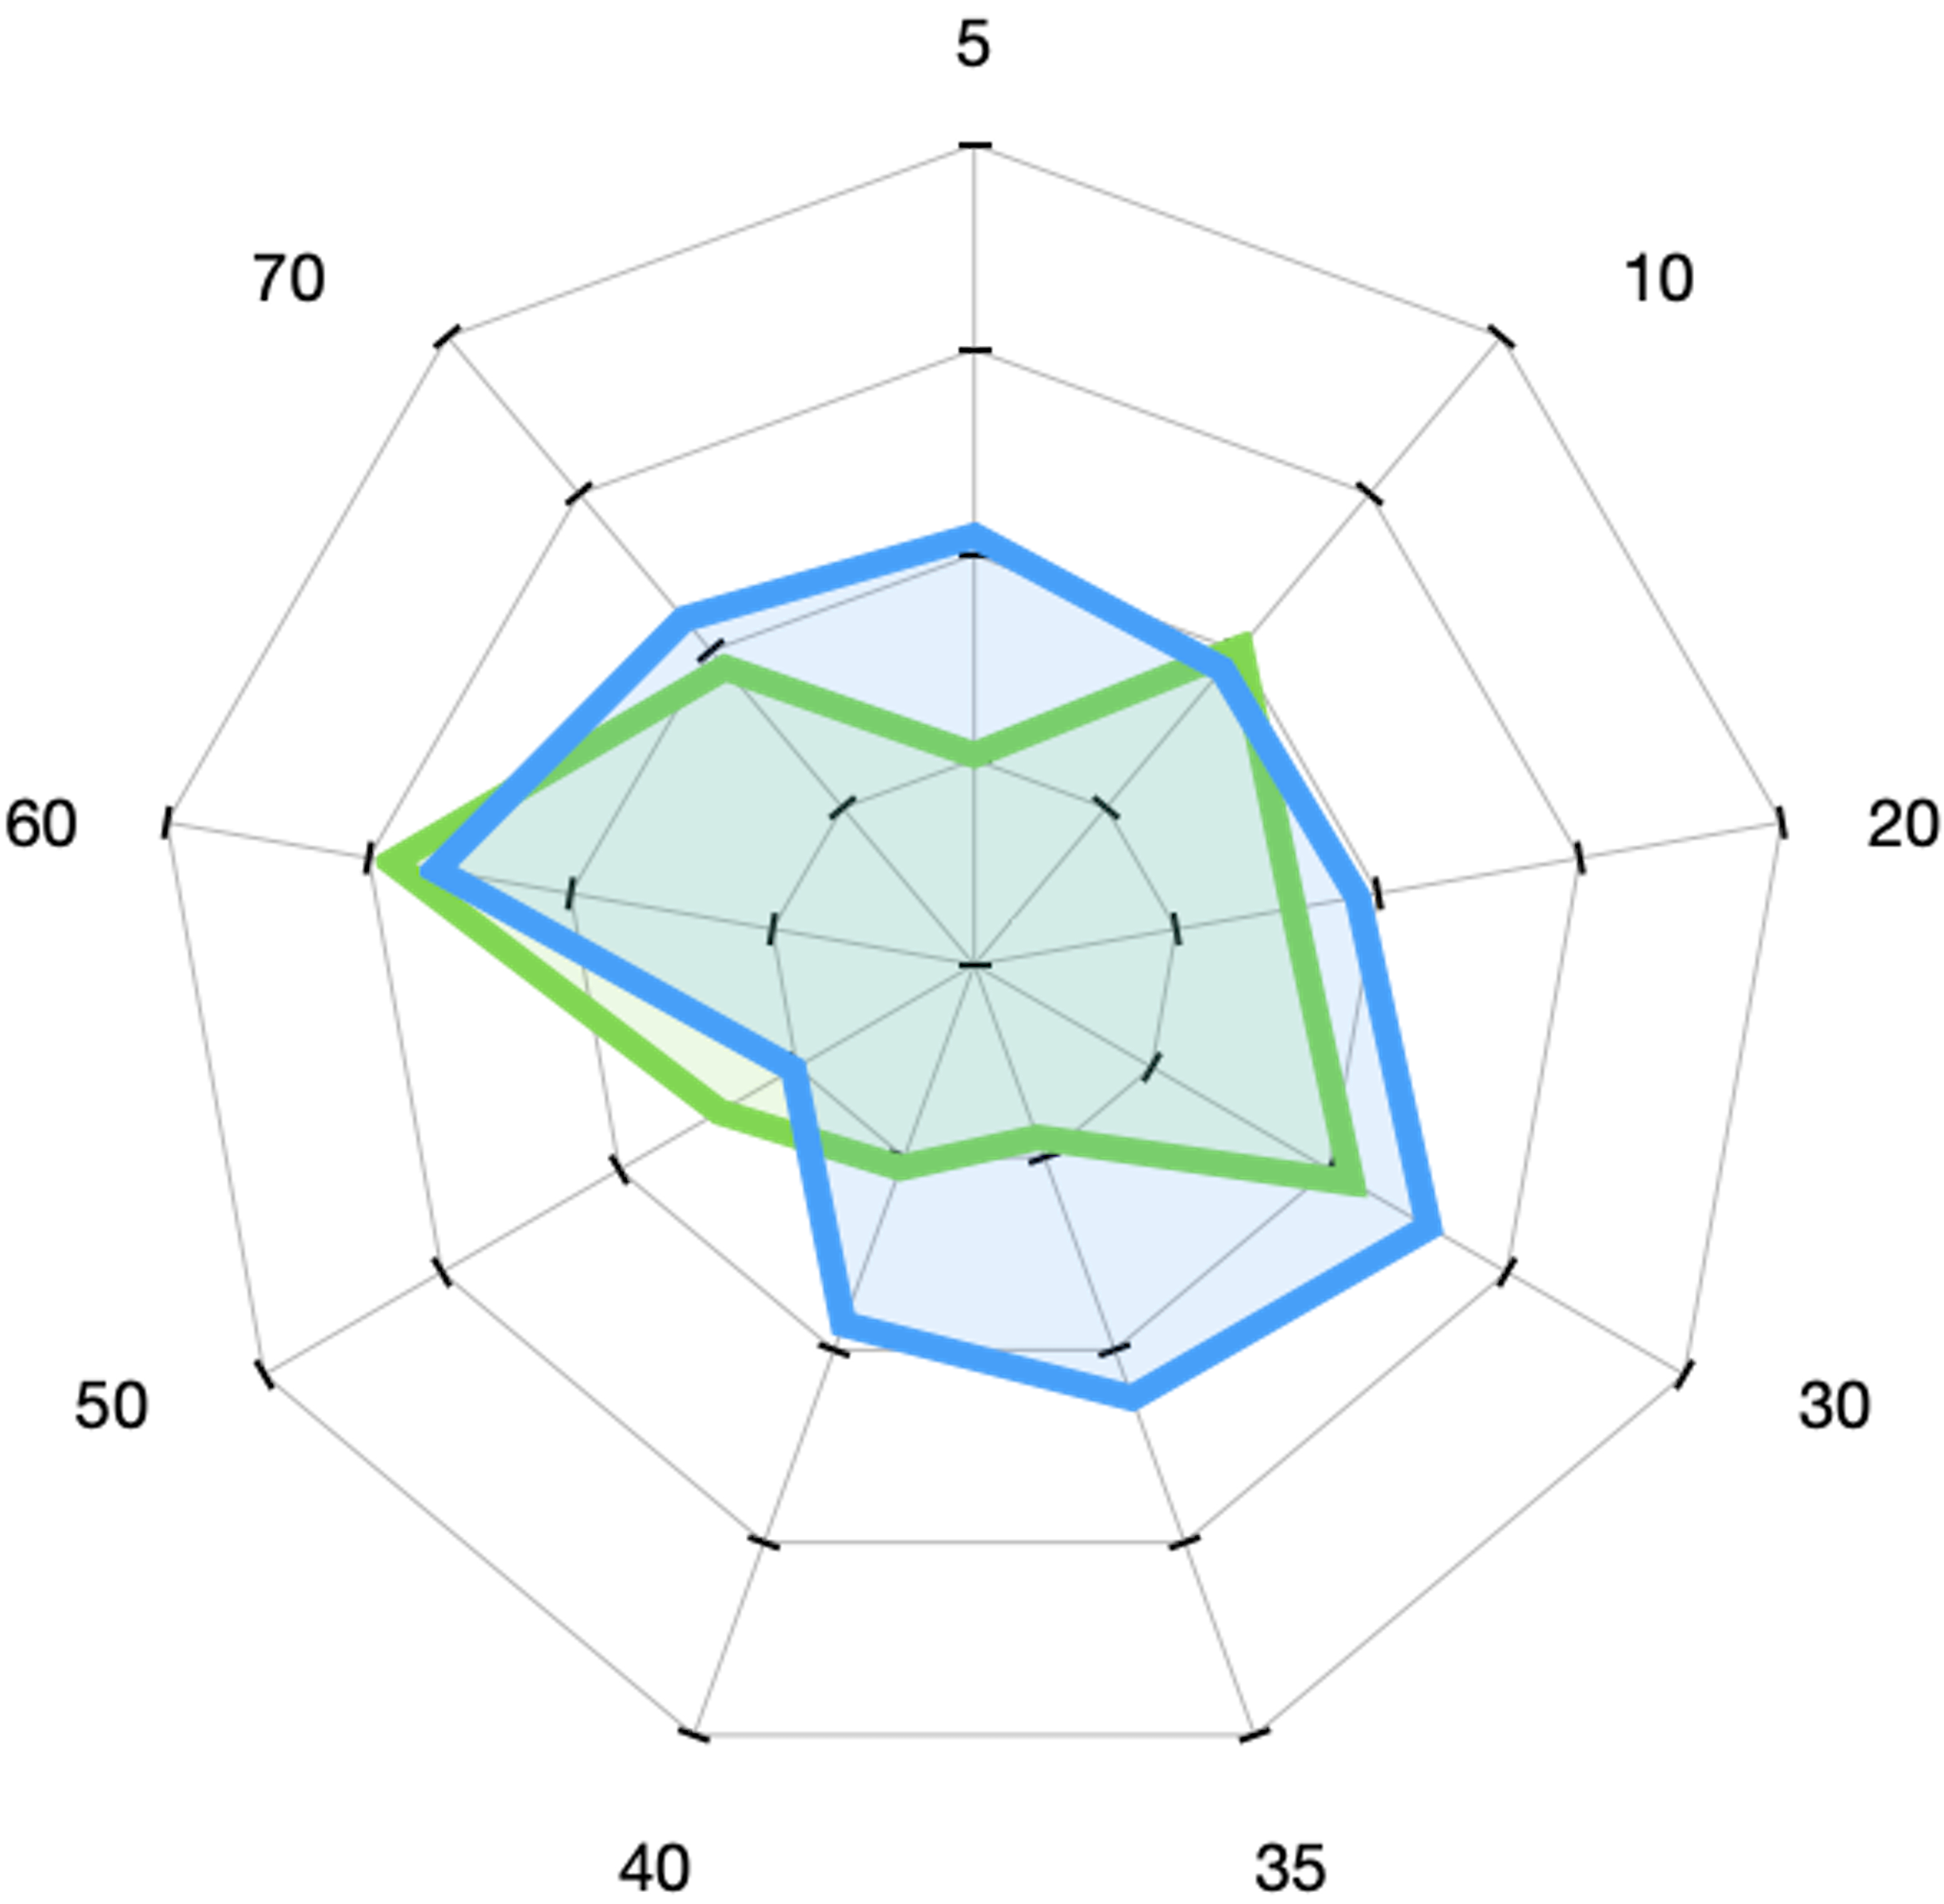
\includegraphics[width=0.4\textwidth, height=0.25\linewidth]{BI-LSTM_RMSE_SPIDER.png}\label{fig:BiLSTM_RMSE_SPIDER}}  
\hfill
\subfloat[GRU Vs Proposed GRU]{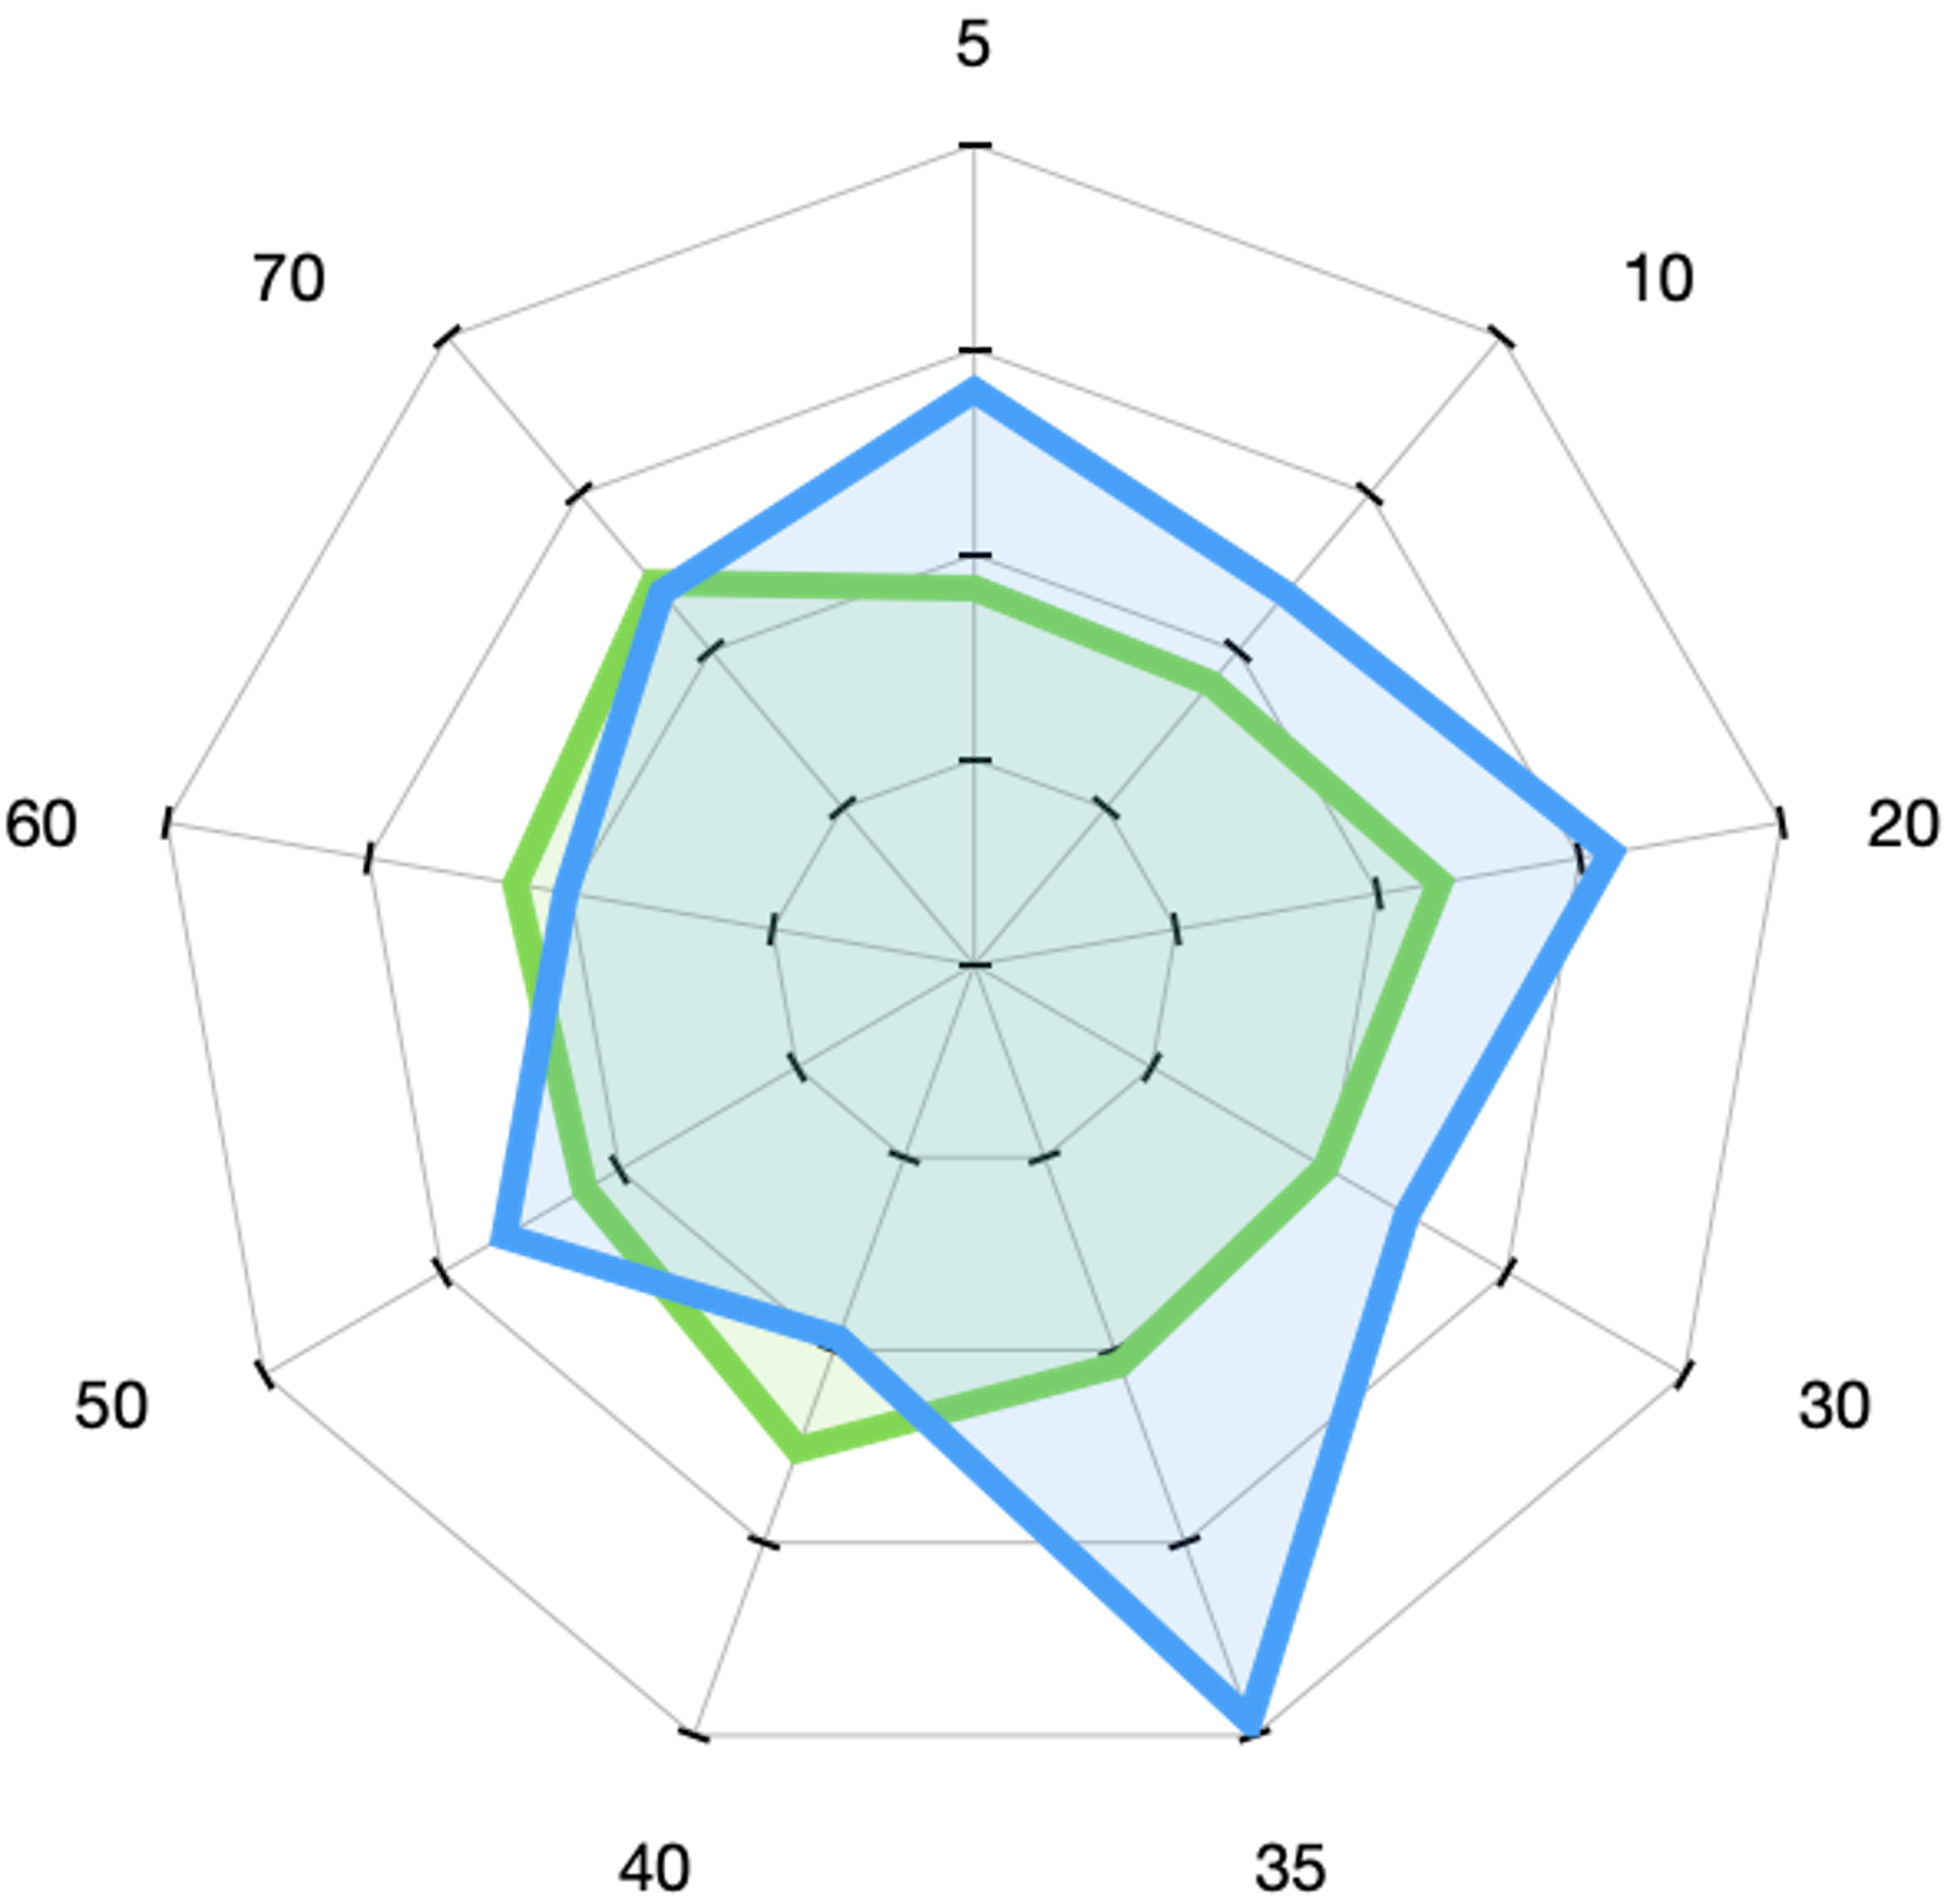
\includegraphics[width=0.4\textwidth, height=0.25\linewidth]{GRU_RMSE_SPIDER.png}\label{fig:GRU_RMSE_SPIDER}}  
  \caption{Comparison of models over RMSE}
  \label{fig:all_models_rmse}
\end{figure} 


\begin{figure}[ht!]
%\centering
\subfloat[LSTM Vs Proposed LSTM]{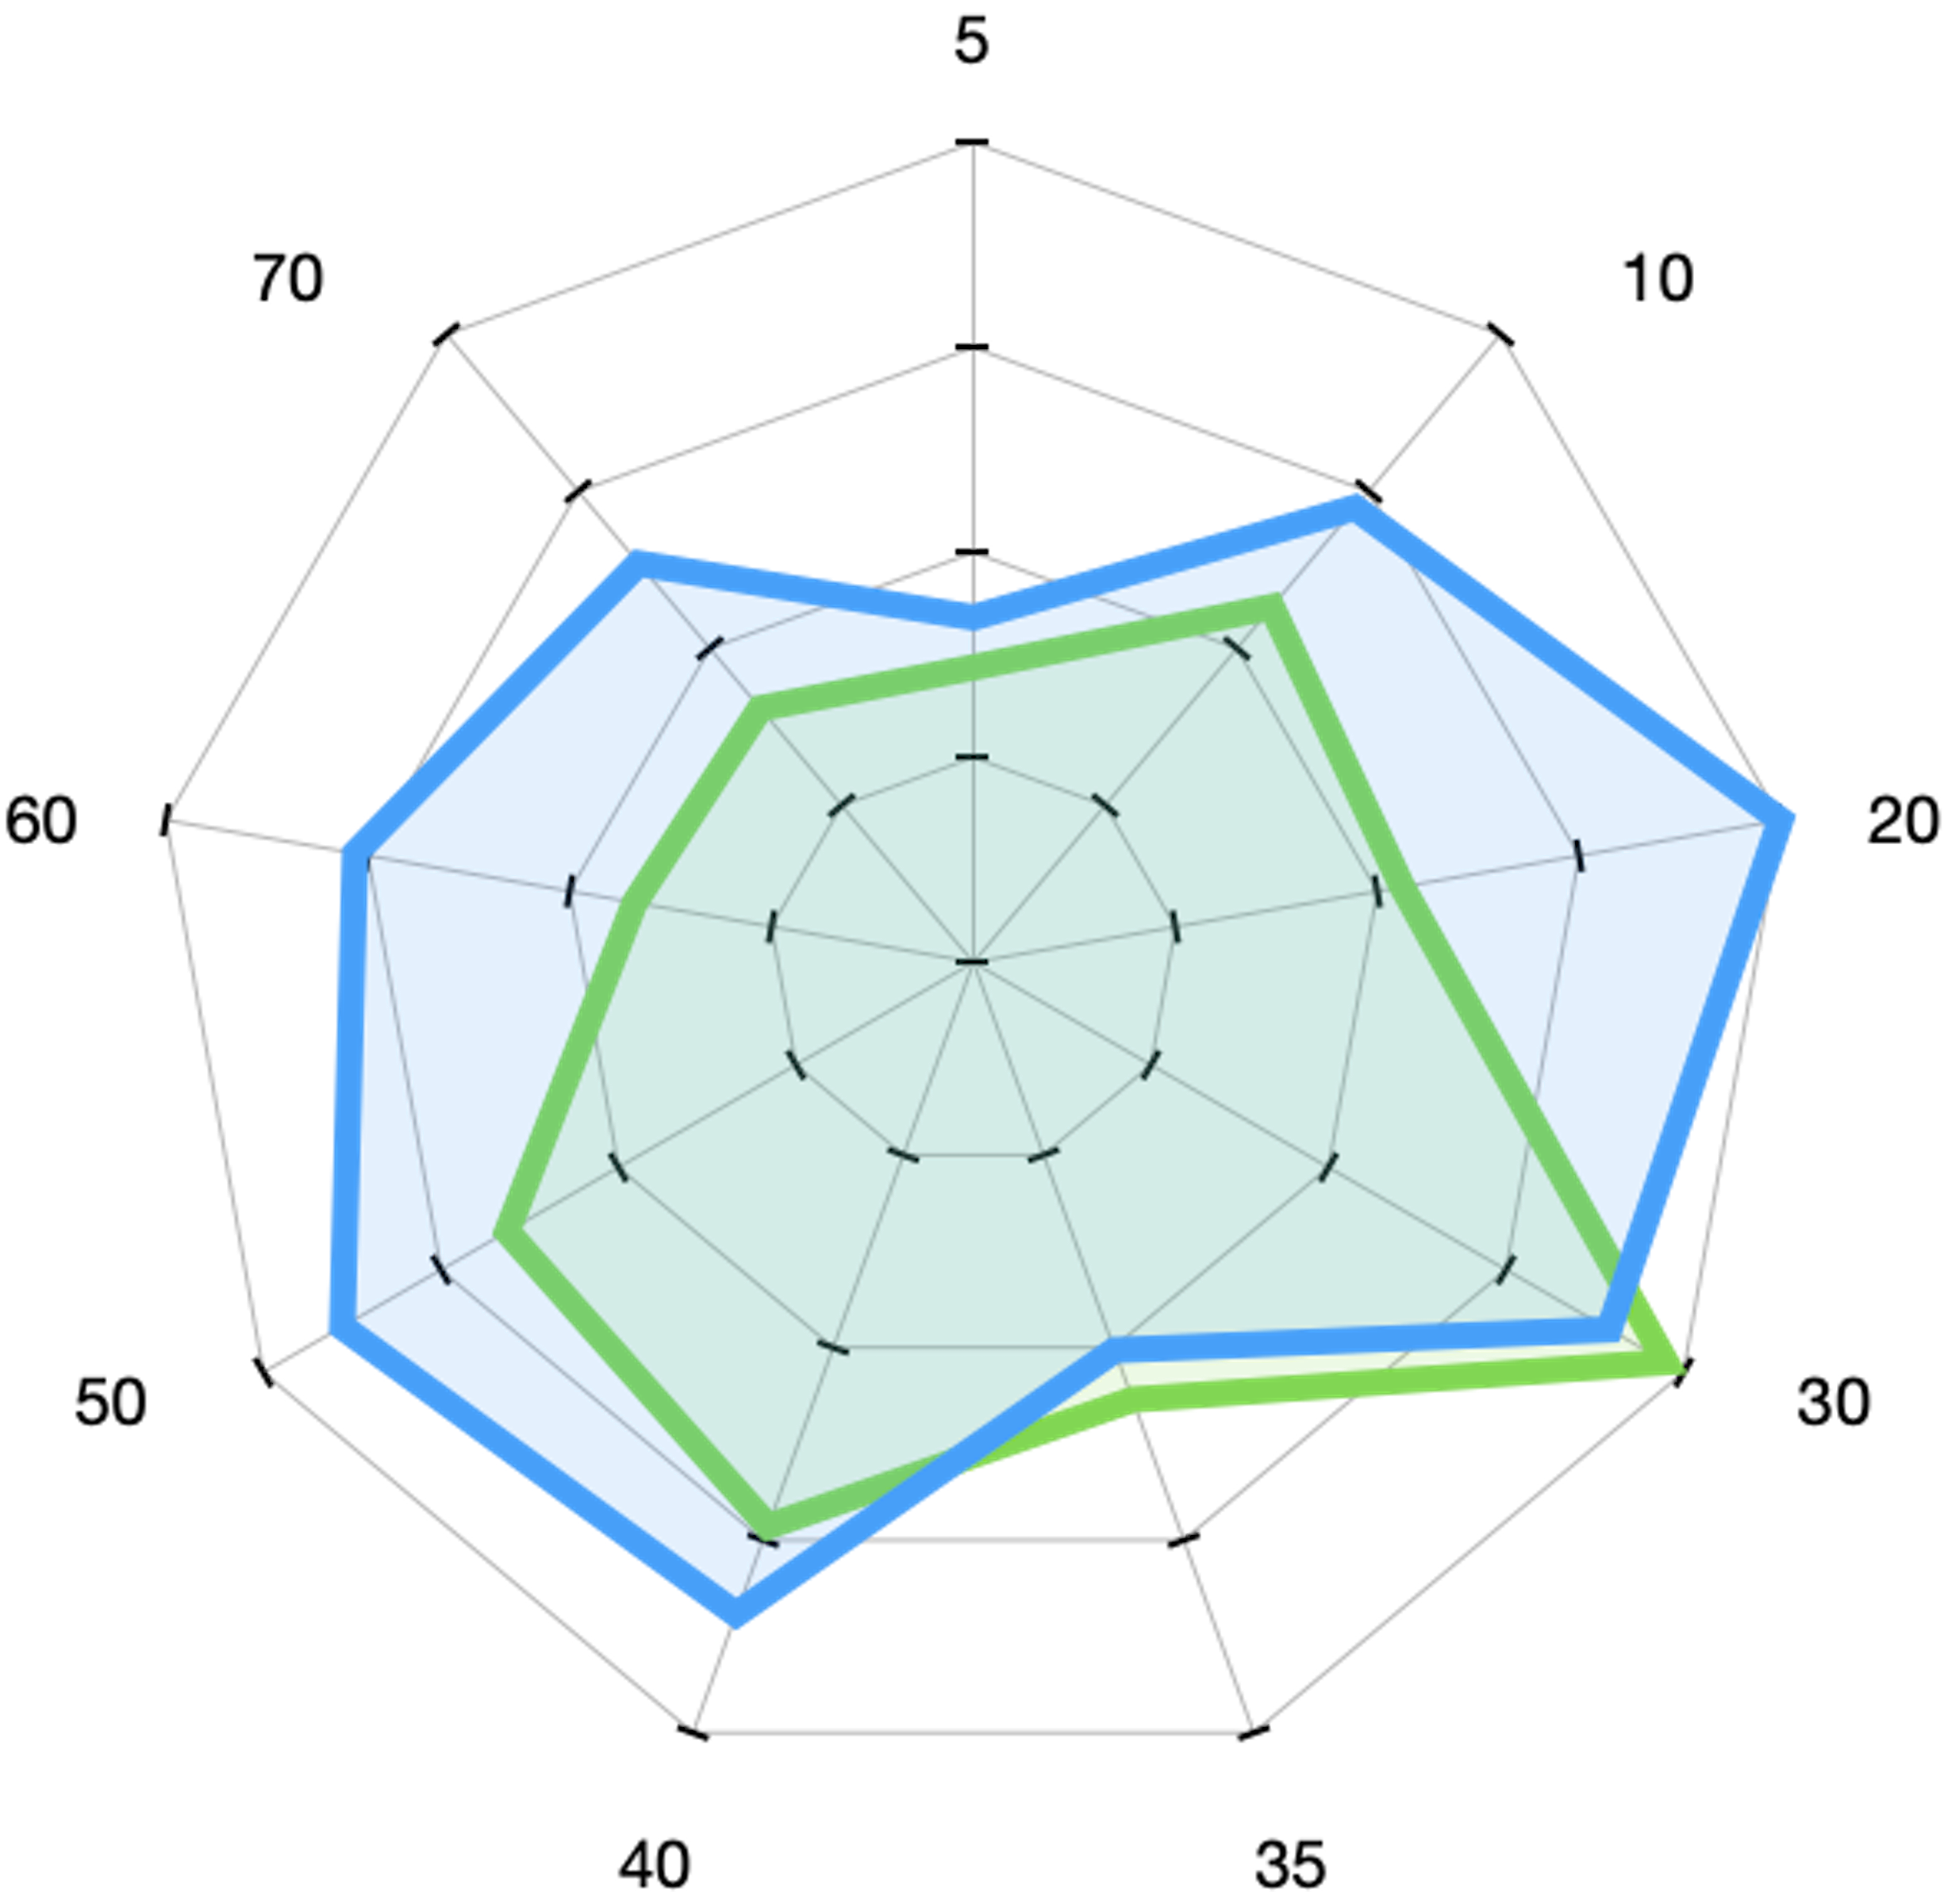
\includegraphics[width=0.4\textwidth, height=0.25\linewidth]{LSTM_RMSE_SPIDER.png}\label{fig:LSTM MAPE SPIDER}}
\hfill
\subfloat[RNN Vs Proposed RNN]{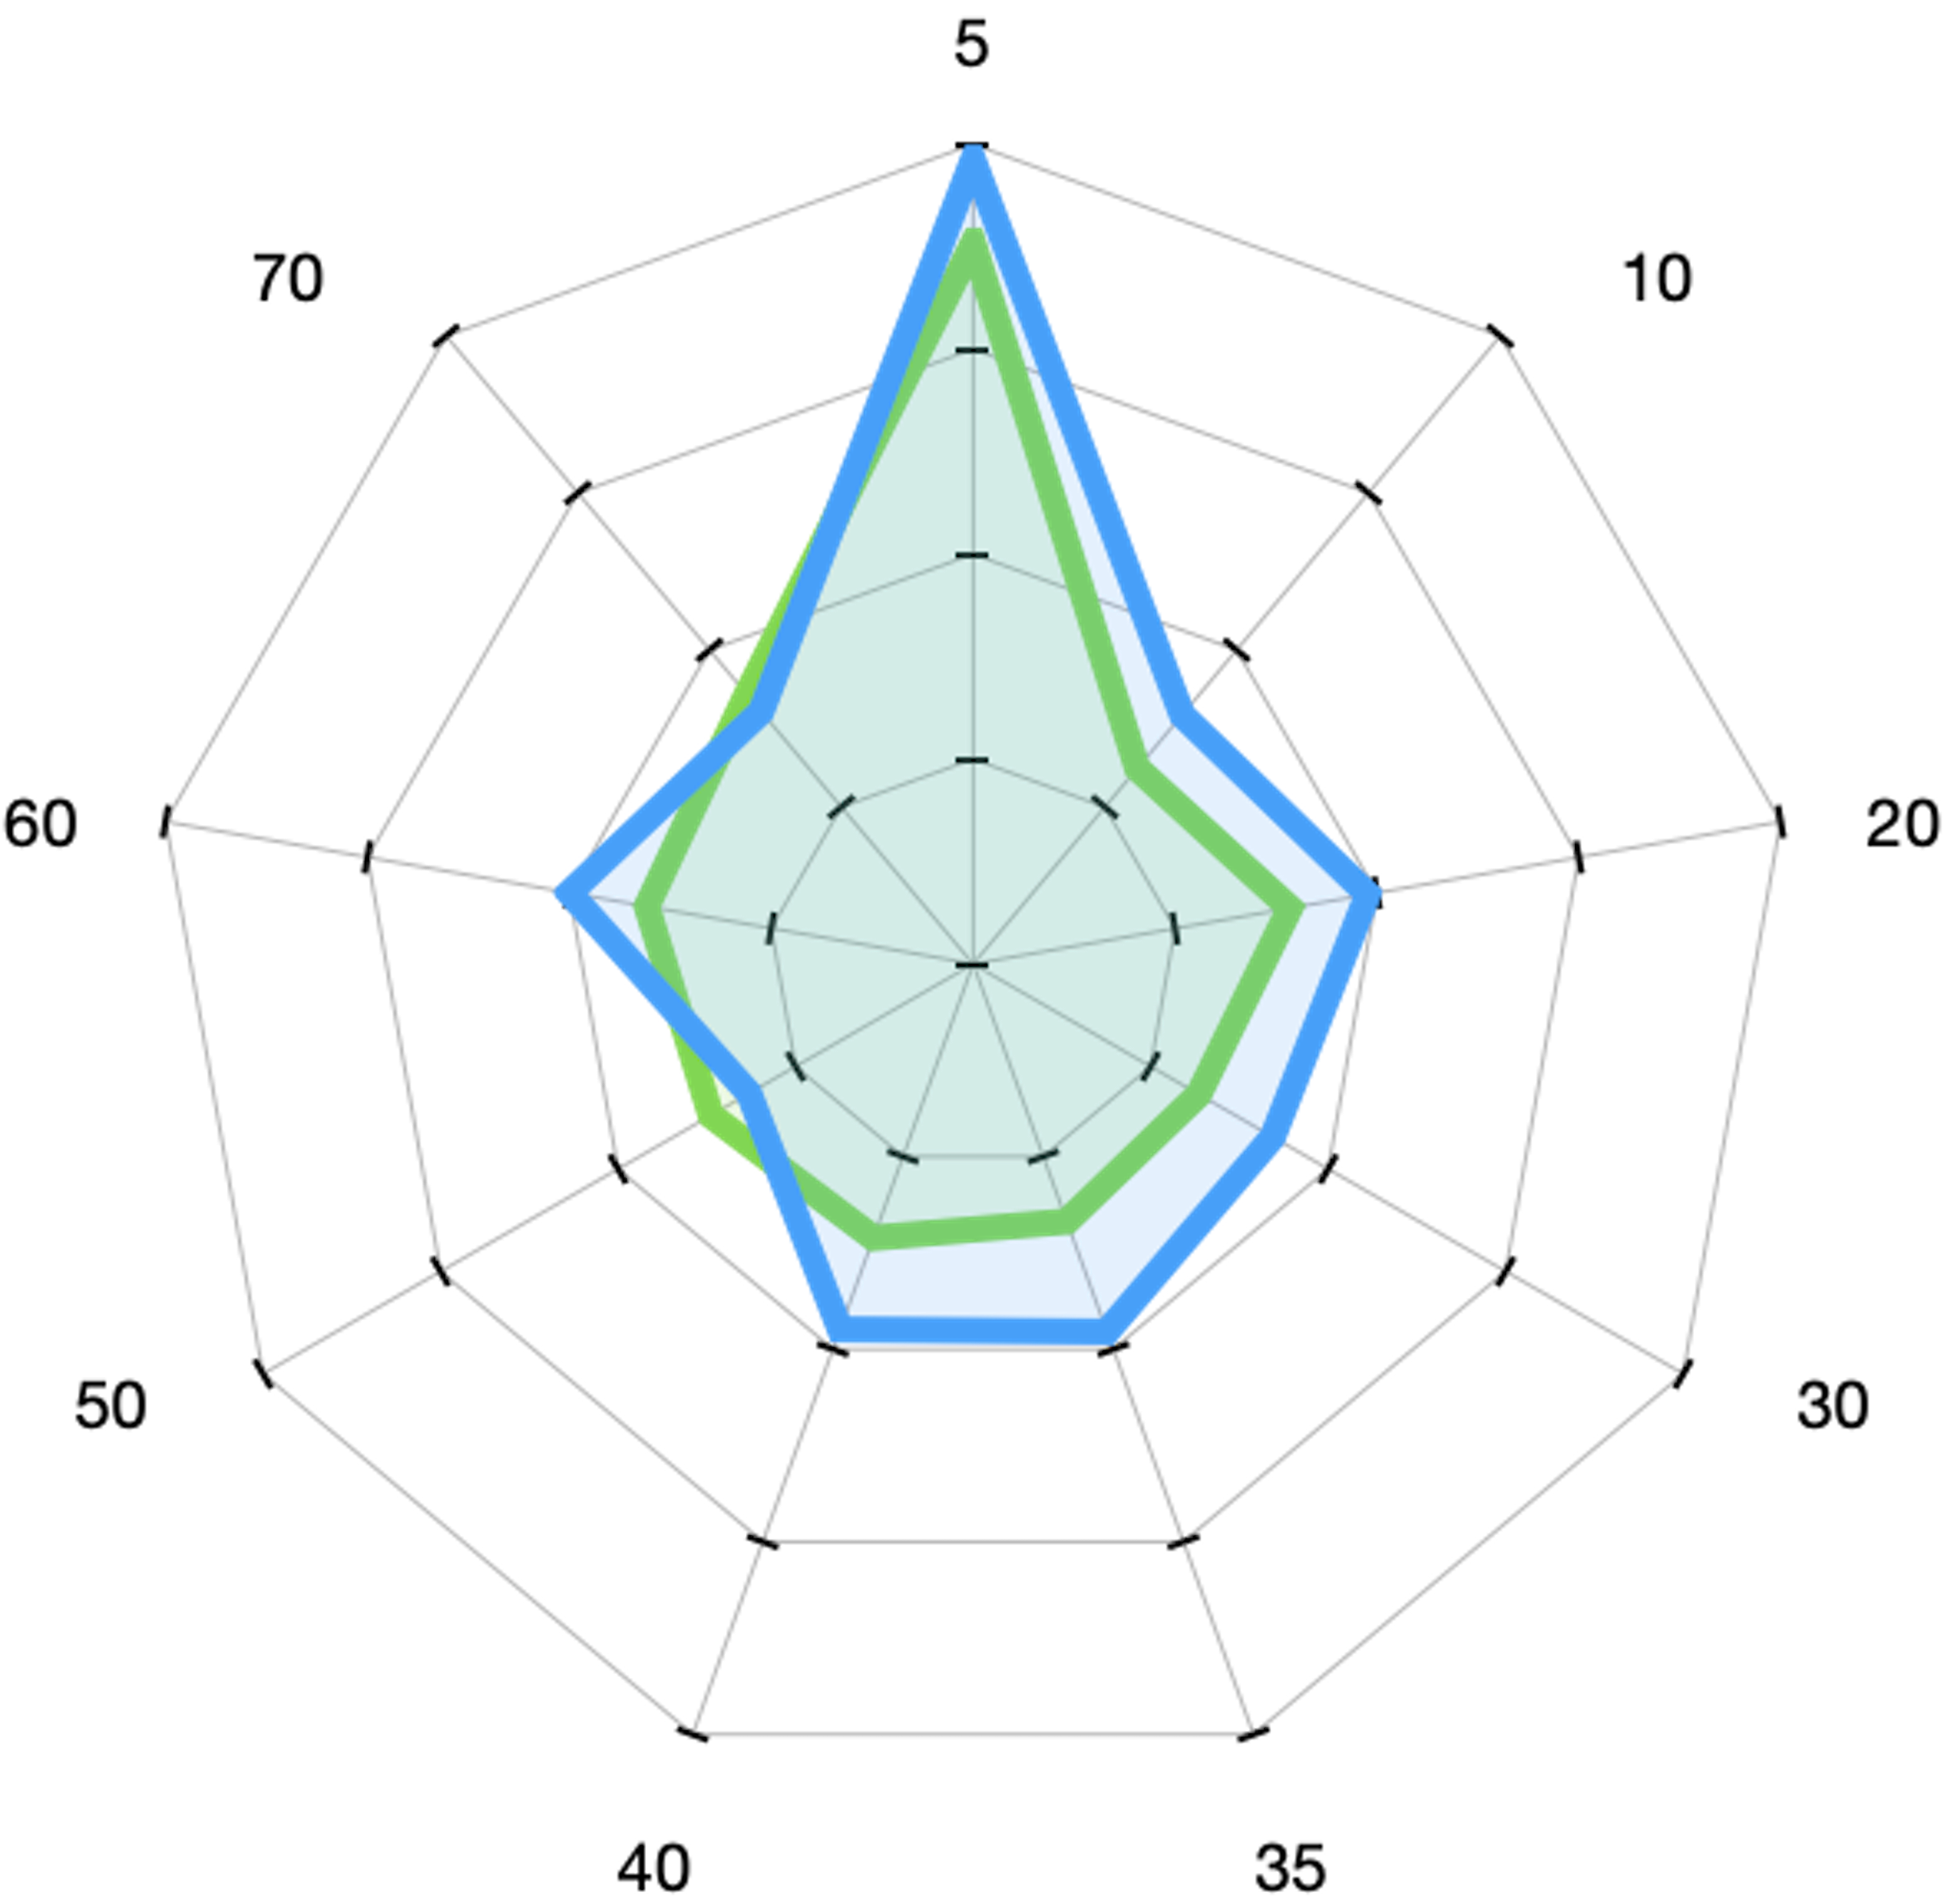
\includegraphics[width=0.4\textwidth, height=0.25\linewidth]{RNN_RMSE_SPIDER.png}\label{fig:RNN_MAPE_SPIDER}}  
\\
\subfloat[BiLSTM Vs Proposed RNN]{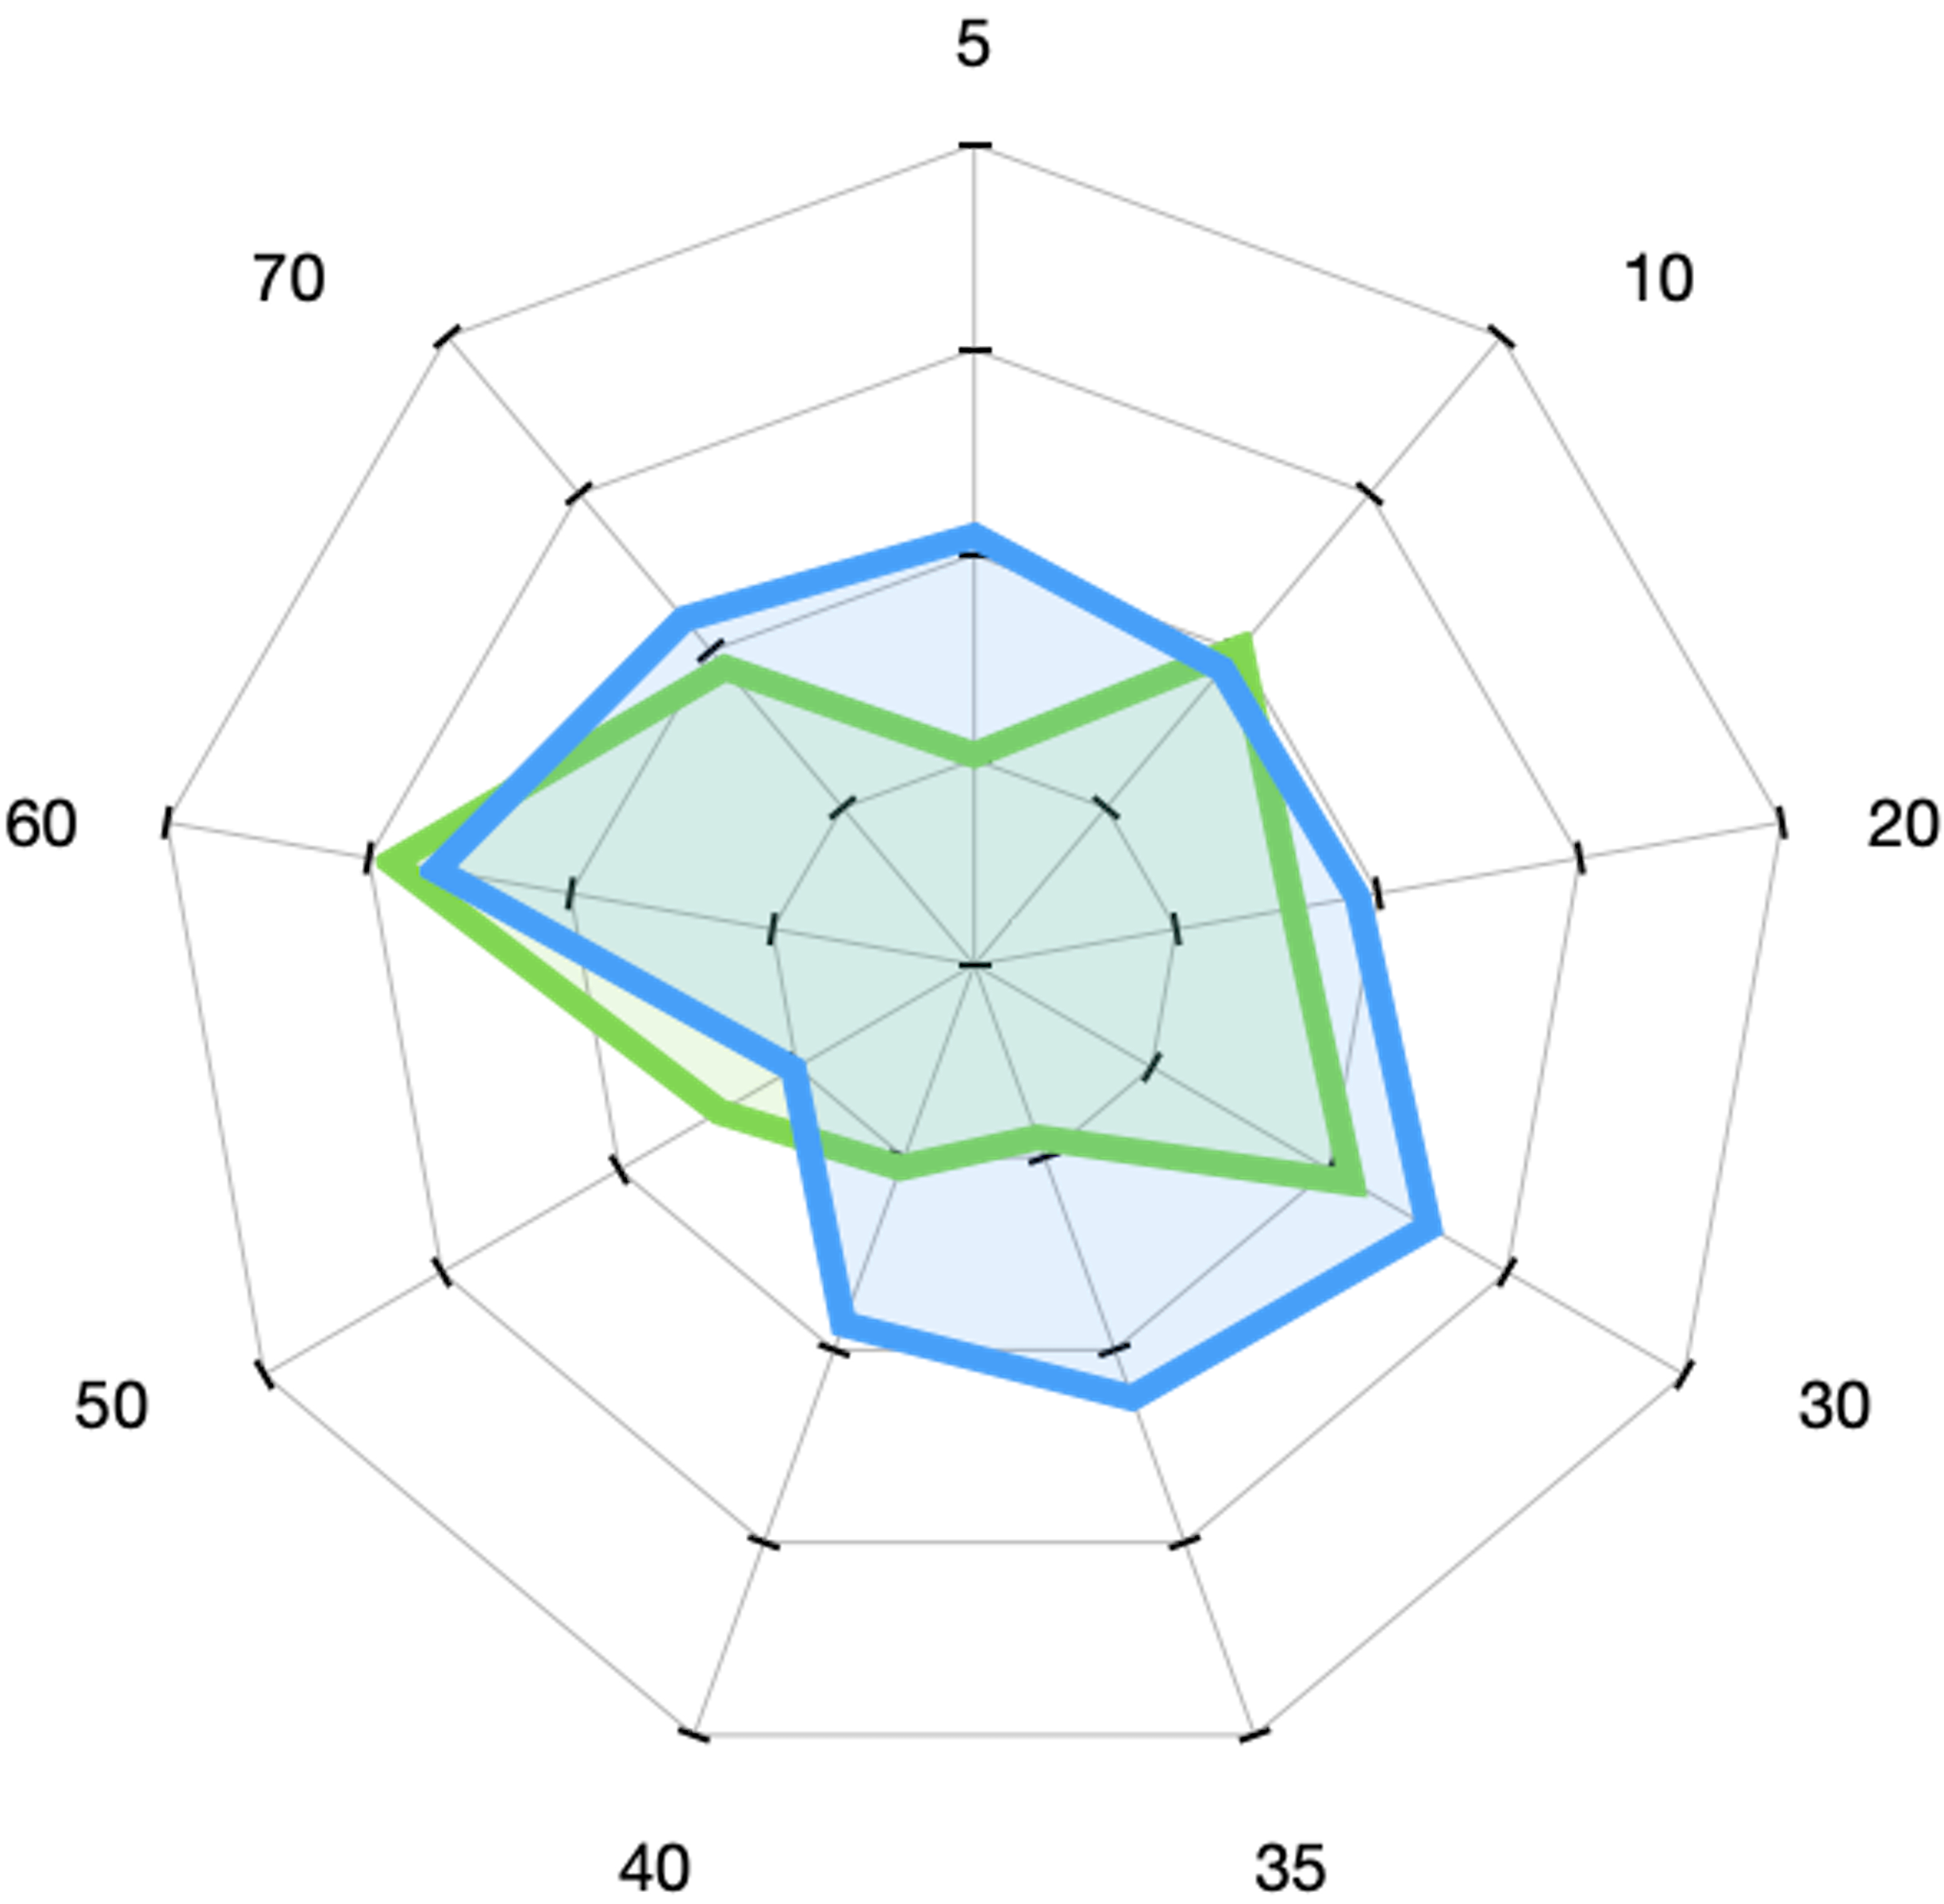
\includegraphics[width=0.4\textwidth, height=0.25\linewidth]{BI-LSTM_RMSE_SPIDER.png}\label{fig:BiLSTM_MAPE_SPIDER}}  
\hfill
\subfloat[GRU Vs Proposed GRU]{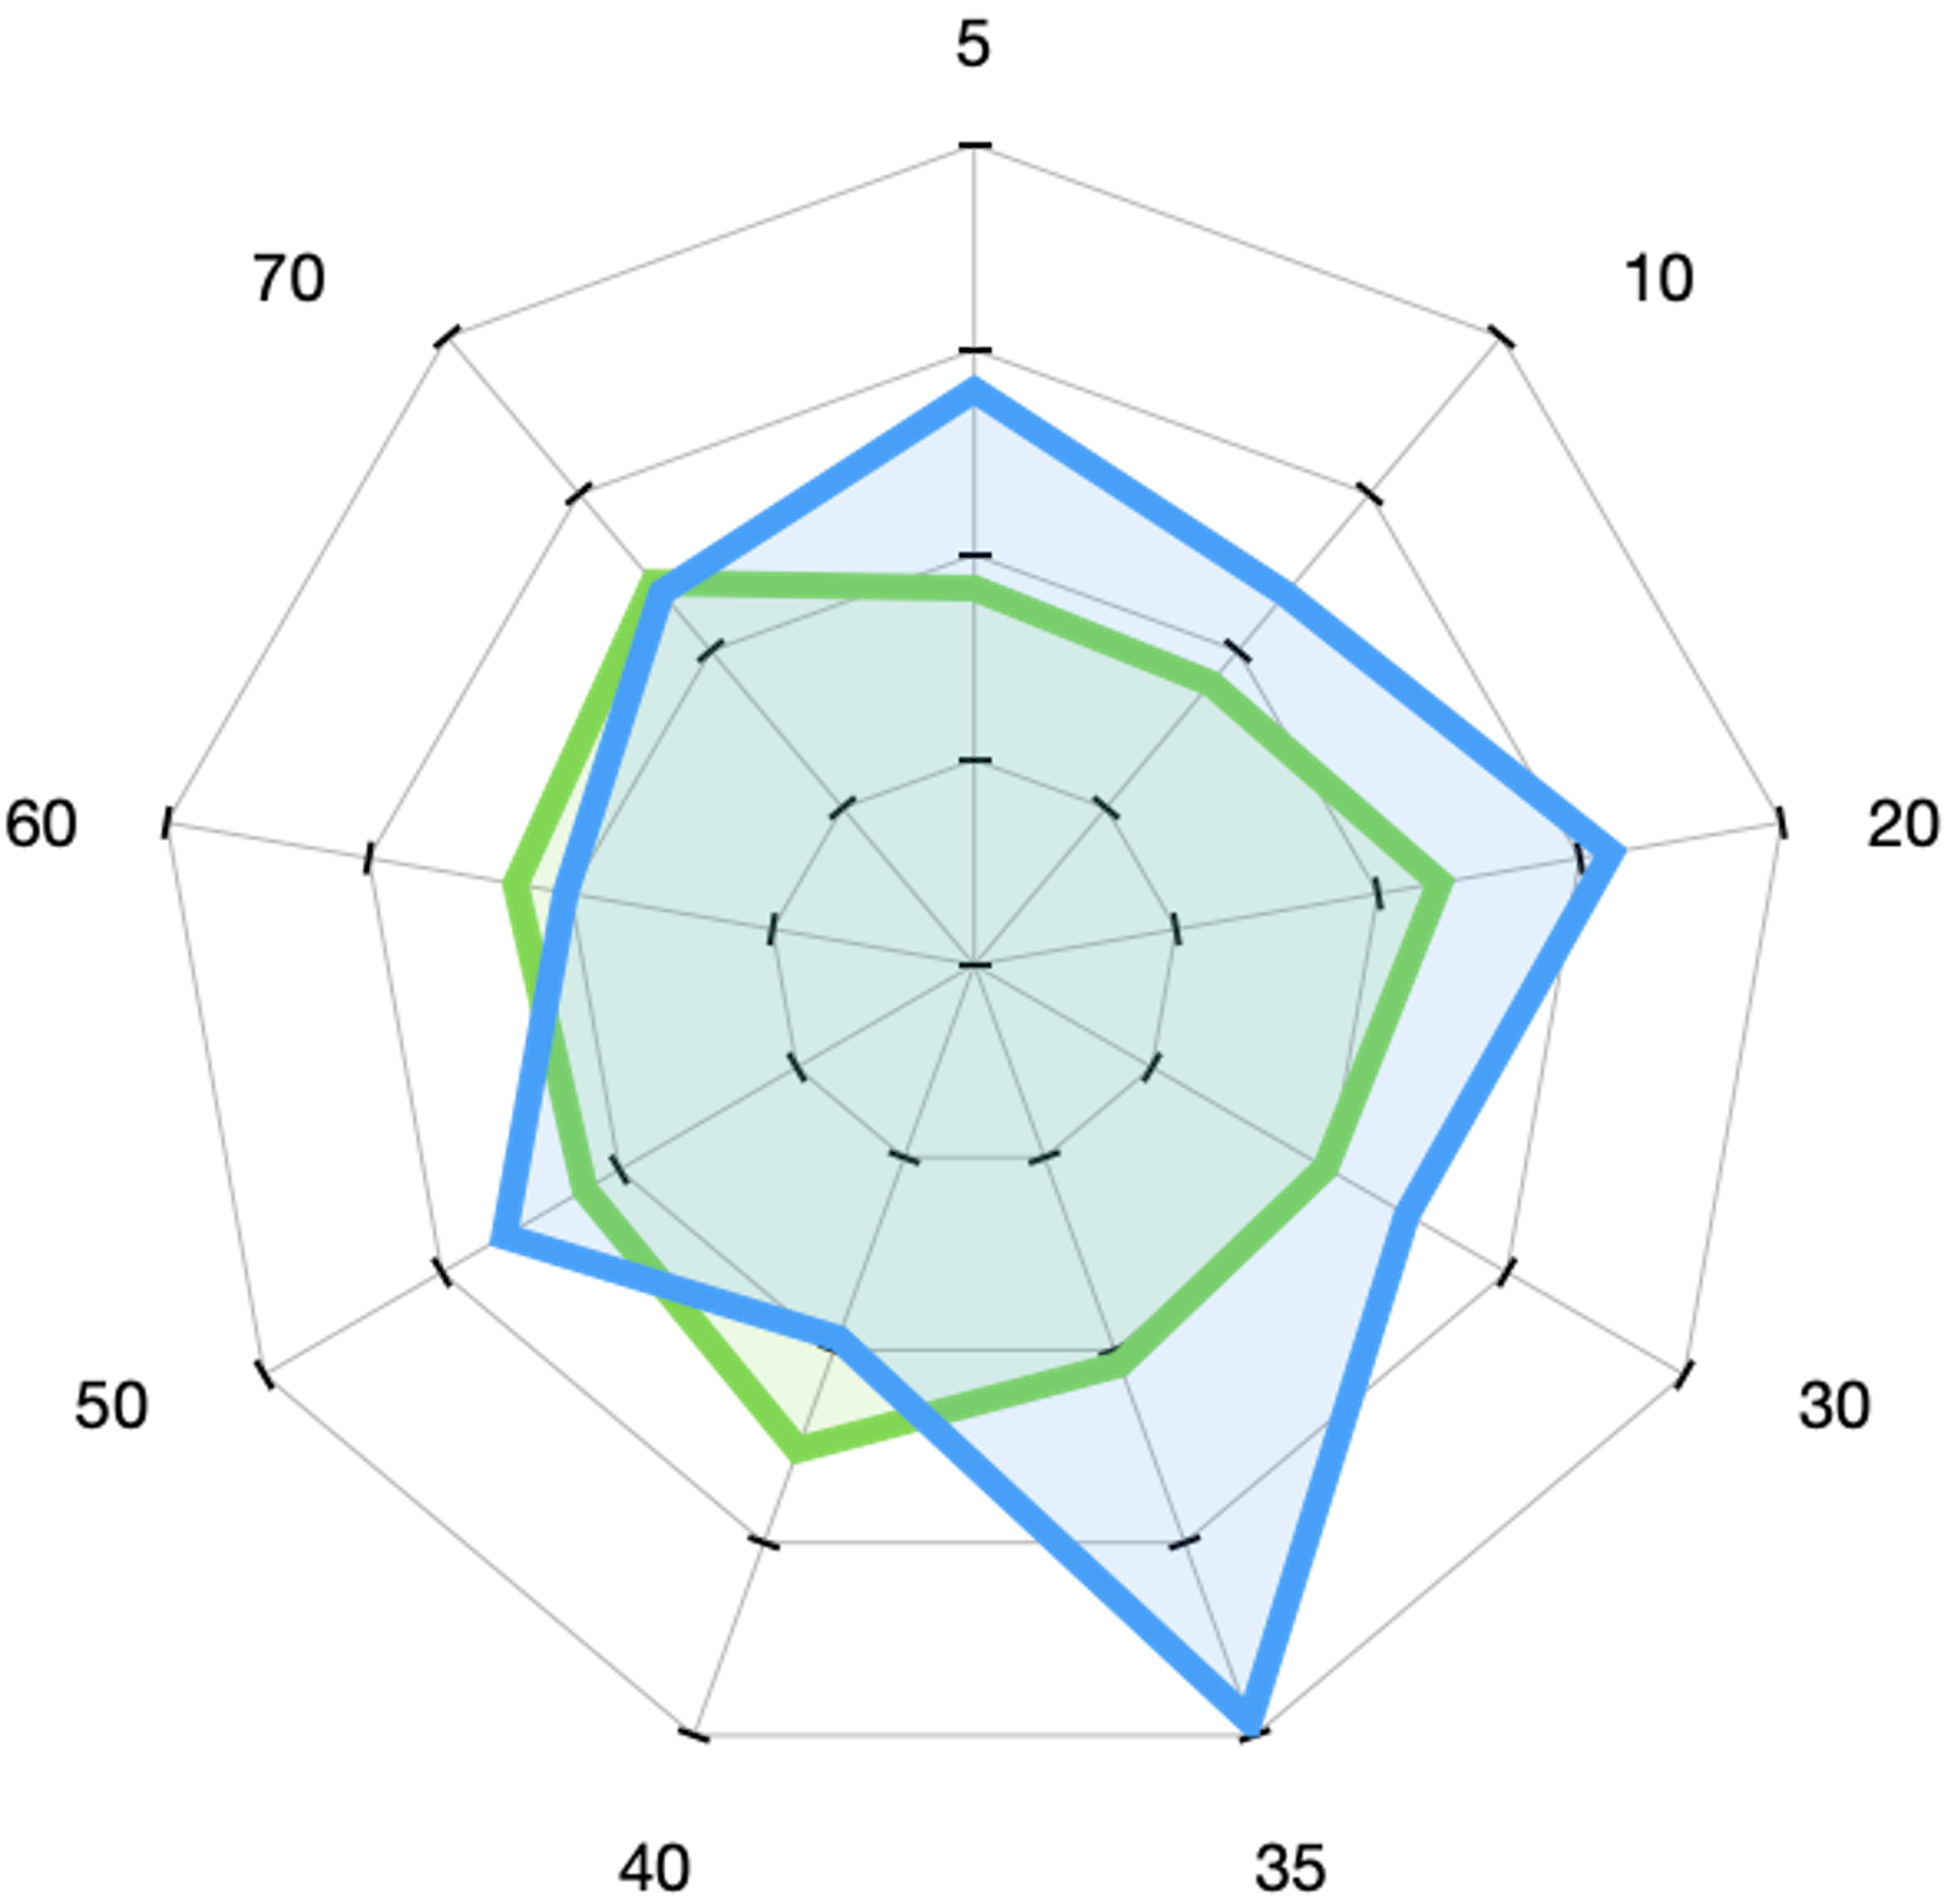
\includegraphics[width=0.4\textwidth, height=0.25\linewidth]{GRU_RMSE_SPIDER.png}\label{fig:GRU_MAPE_SPIDER}}  
  \caption{Comparison of models over MAPE}
  \label{fig:all_models_rmse}
\end{figure} 

\begin{figure}[ht!]
\centering
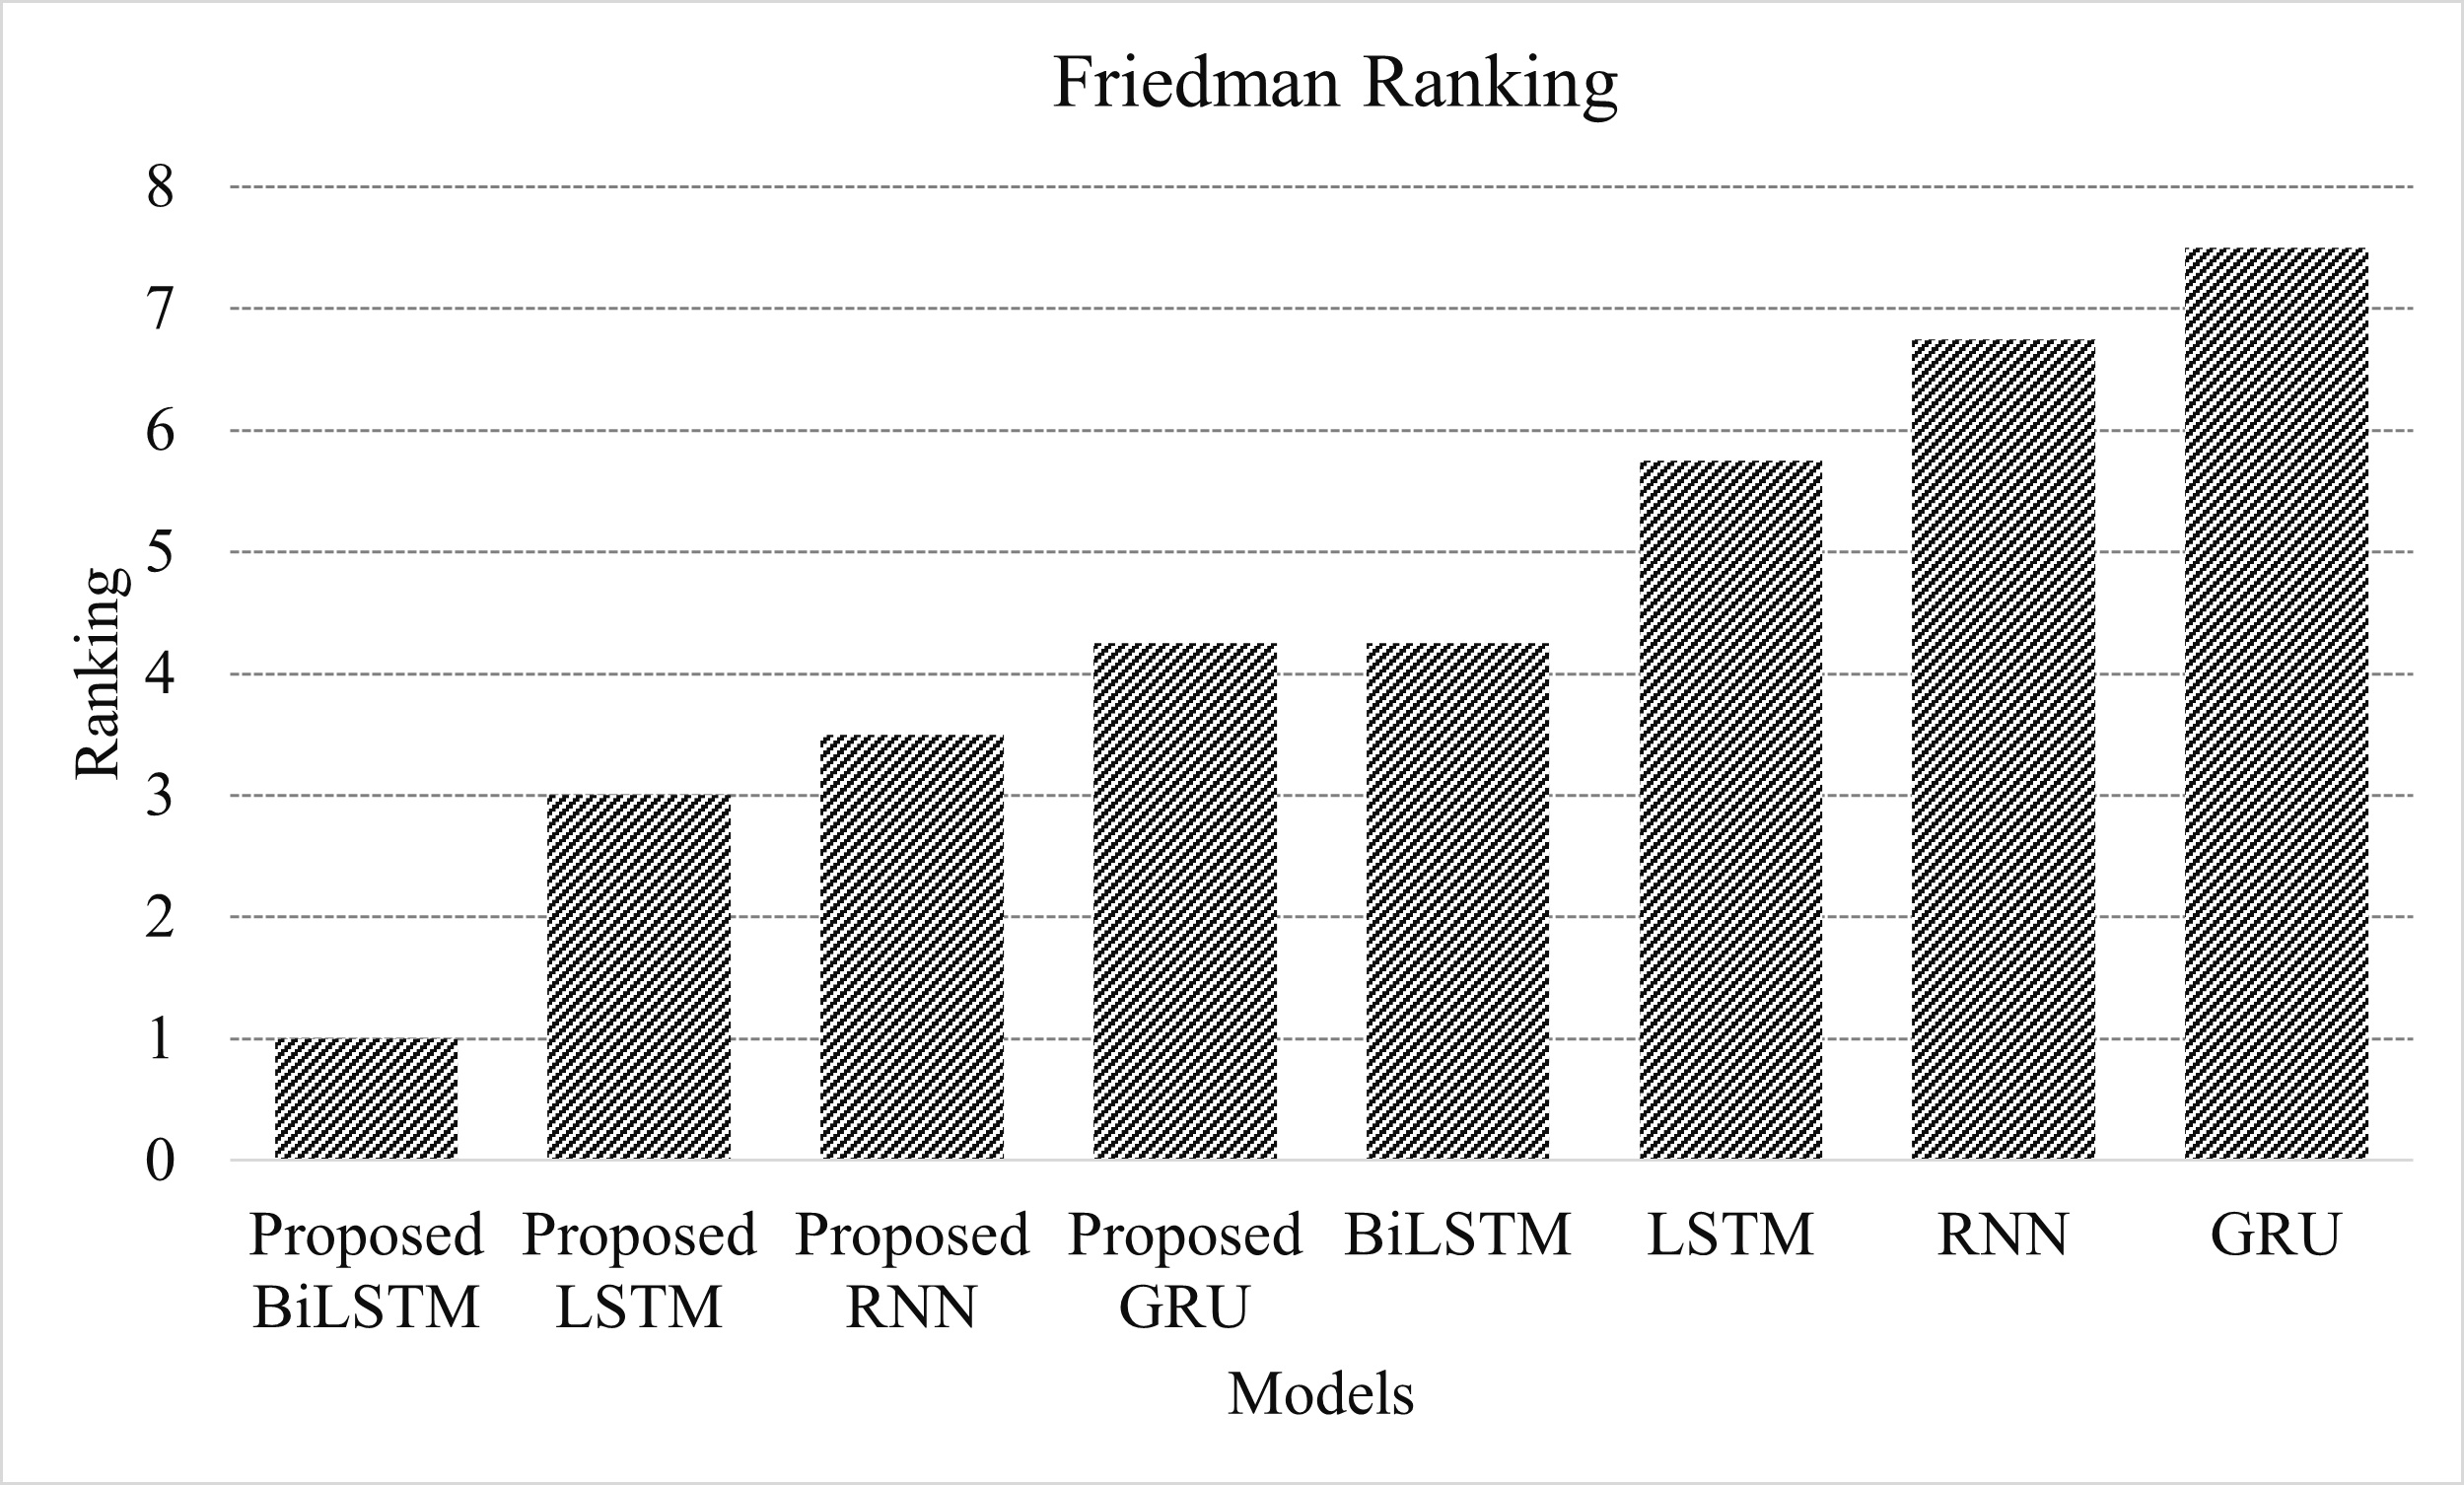
\includegraphics[width=0.9\textwidth, height=0.6\linewidth]{Graph.jpeg}
\label{fig:Friedman}
 \caption{Friedman Ranking of all models}
 \end{figure} 
%\centering
\pagebreak
Figures \ref{fig:LSTM MAE SPIDER}, \ref{fig:LSTM MAE SPIDER} and \ref{fig:LSTM MAE SPIDER} represents the experiment results for the LSTM where it can be observed that MAE , RMSE and MSE has improved respectively. The improvement in each case is for the eight out of nine experimented shifts which validates the performance of the proposed method. Similarly, Figure \ref{fig:RNN_MAE_SPIDER}, \ref{fig:RNN_RMSE_SPIDER}, \ref{fig:RNN_MSE_SPIDER} depicts the comparative performances for RNN over MAE, RMSE and MSE respectively. The improvement can be observed for most of the cases over all three evaluation metrics. In the similar pattern, Figure \ref{fig:BiLSTM_MAE_SPIDER}, \ref{fig:BiLSTM_RMSE_SPIDER} and \ref{fig:BiLSTM_MSE_SPIDER} represents the comparative view of the proposed method over the BiLSTM model for all experimented measures namely MAE, RMSE and MSE respectively. For every performance metric, improvement can be observed over the traditional approach. The perfor 
 mances comparison over MAE , RMSE and MSE for GRU model is depicted in Figure \ref{fig:GRU_MAE_SPIDER}, \ref{fig:GRU_RMSE_SPIDER} and \ref{fig:GRU_MSE_SPIDER} respectively. These figures also suggest an improvement in the performance of GRU after the implementation of the proposed model.
%\section{This is an example for first level head---section head}\label{sec3}
\begin{table}[ht!]
\begin{tabular}{l|lllll}
\hline
\\
Models& MSE & RMSE & MAE & MAPE & Friedman Ranking\\  
\hline
\\
LSTM            & 7   & 7    & 6   & 3  & 5.75  \\
GRU             & 8   & 8    & 8   & 6  &7.5  \\
BiLSTM          & 4   & 4    & 4   & 5  &4.25  \\
RNN             & 6   & 6    & 7   & 8  &6.75  \\
Proposed LSTM   & 3   & 3    & 2   & 4  & 3  \\
Proposed GRU    & 5   & 5    & 5   & 2   &4.25 \\
Proposed BiLSTM & 1   & 1    & 1   & 1 &1   \\
Proposed RNN    & 2   & 2    & 3   & 7  &3.5  \\ \hline
\end{tabular}
\caption{Ranking of Different Models on the basis of performance measures}
\label{tab:Friedman}
\end{table}
Non Parametric Friedman Ranking of all experimented models is representated in Table \ref{tab:Friedman}

%\begin{table}[!htp]
%\centering
%\begin{tabular}{|c|c|}\hline
%Algorithm&Ranking\\\hline
%LSTM & 5.75\\
%GRU & 7.5\\
%BiLSTM & 4.25\\
%RNN & 6.75\\
%Proposed LSTM & 3\\
%Proposed GRU & 4.25\\
%Proposed BiLSTM & 1\\
%Proposed RNN & 3.5\\
%\hline
%\end{tabular}
%\caption{Average Rankings of the algorithms}
%\label{tab:Friedman}
%\end{table}
Adjusted p-values for $\alpha$=0.05 is represented in Table \ref{tab:pvalue}
%\begin{table}[!htp]
%\centering\scriptsize
%\begin{tabular}{cccc}
%$i$&algorithms&$z=(R_0 - R_i)/SE$&$p$\\
%\hline6&GRU vs. BiLSTM&2.738613&0.00617\\
%5&LSTM vs. BiLSTM&1.917029&0.055234\\
%4&BiLSTM vs. RNN&1.917029&0.055234\\
%3&LSTM vs. GRU&0.821584&0.411314\\
%2&GRU vs. RNN&0.821584&0.411314\\
%1&LSTM vs. RNN&0&1\\
%\hline
%\end{tabular}
%\caption{P-values Table for $\alpha=0.05$}
%\label{tab:pvalue}
%\end{table}

\begin{table}[!htbp]
\centering\scriptsize
\begin{tabular}{cccc}
\hline
$i$&algorithms&$z=(R_0 - R_i)/SE$&$p$\\
\hline28&GRU vs. Proposed BiLSTM&3.752777&0.000175\\
27&RNN vs. Proposed BiLSTM&3.319764&0.000901\\
26&LSTM vs. Proposed BiLSTM&2.742414&0.006099\\
25&GRU vs. Proposed LSTM&2.598076&0.009375\\
24&GRU vs. Proposed RNN&2.309401&0.020921\\
23&RNN vs. Proposed LSTM&2.165064&0.030383\\
22&GRU vs. BiLSTM&1.876388&0.060602\\
21&GRU vs. Proposed GRU&1.876388&0.060602\\
20&BiLSTM vs. Proposed BiLSTM&1.876388&0.060602\\
19&RNN vs. Proposed RNN&1.876388&0.060602\\
18&Proposed GRU vs. Proposed BiLSTM&1.876388&0.060602\\
17&LSTM vs. Proposed LSTM&1.587713&0.112351\\
16&BiLSTM vs. RNN&1.443376&0.148915\\
15&RNN vs. Proposed GRU&1.443376&0.148915\\
14&Proposed BiLSTM vs. Proposed RNN&1.443376&0.148915\\
13&LSTM vs. Proposed RNN&1.299038&0.193931\\
12&Proposed LSTM vs. Proposed BiLSTM&1.154701&0.248213\\
11&LSTM vs. GRU&1.010363&0.312321\\
10&LSTM vs. BiLSTM&0.866025&0.386476\\
9&LSTM vs. Proposed GRU&0.866025&0.386476\\
8&BiLSTM vs. Proposed LSTM&0.721688&0.470486\\
7&Proposed LSTM vs. Proposed GRU&0.721688&0.470486\\
6&LSTM vs. RNN&0.57735&0.563703\\
5&GRU vs. RNN&0.433013&0.665006\\
4&BiLSTM vs. Proposed RNN&0.433013&0.665006\\
3&Proposed GRU vs. Proposed RNN&0.433013&0.665006\\
2&Proposed LSTM vs. Proposed RNN&0.288675&0.77283\\
1&BiLSTM vs. Proposed GRU&0&1\\
\hline
\end{tabular}
\caption{P-values Table for $\alpha=0.05$}
\label{tab:pvalue}
\end{table}
\pagebreak

\section{Conclusion}
In this study, a deep learning approach has been utilized to forecast the temperature.
\bmhead{Acknowledgments}

Acknowledgments are not compulsory. Where included they should be brief. Grant or contribution numbers may be acknowledged.

Please refer to Journal-level guidance for any specific requirements.

%\section*{Declarations}

%Some journals require declarations to be submitted in a standardised format. Please check the Instructions for Authors of the journal to which you are submitting to see if you need to complete this section. If yes, your manuscript must contain the following sections under the heading `Declarations':

%\begin{itemize}
%\item Funding
%\item Conflict of interest/Competing interests (check journal-specific guidelines for which heading to use)
%\item Ethics approval 
%\item Consent to participate
%\item Consent for publication
%\item Availability of data and materials
%\item Code availability 
%\item Authors' contributions
%\end{itemize}

%\noindent
%If any of the sections are not relevant to your manuscript, please include the heading and write `Not applicable' for that section. 

%%===================================================%%
%% For presentation purpose, we have included        %%
%% \bigskip command. please ignore this.             %%
%%===================================================%%
%\bigskip
%\begin{flushleft}%
%Editorial Policies for:

%\bigskip\noindent
%Springer journals and proceedings: \url{https://www.springer.com/gp/editorial-policies}

%\bigskip\noindent
%Nature Portfolio journals: \url{https://www.nature.com/nature-research/editorial-policies}

%\bigskip\noindent
%\textit{Scientific Reports}: \url{https://www.nature.com/srep/journal-policies/editorial-policies}

%\bigskip\noindent
%BMC journals: %\url{https://www.biomedcentral.com/getpublished/editorial-policies}
%\end{flushleft}

%\begin{appendices}

%\section{Section title of first appendix}\label{secA1}

%An appendix contains supplementary information that is not an essential part of the text itself but which may be helpful in providing a more comprehensive understanding of the research problem or it is information that is too cumbersome to be included in the body of the paper.
%\end{appendices}
\bibliography{sn-bibliography}% common bib file
%% if required, the content of .bbl file can be included here once bbl is generated
%%\input sn-article.bbl


\end{document}
